%% 
%% Copyright 2019-2020 Elsevier Ltd
%% 
%% This file is part of the 'CAS Bundle'.
%% --------------------------------------
%% 
%% It may be distributed under the conditions of the LaTeX Project Public
%% License, either version 1.2 of this license or (at your option) any
%% later version.  The latest version of this license is in
%%    http://www.latex-project.org/lppl.txt
%% and version 1.2 or later is part of all distributions of LaTeX
%% version 1999/12/01 or later.
%% 
%% The list of all files belonging to the 'CAS Bundle' is
%% given in the file `manifest.txt'.
%% 
%% Template article for cas-sc documentclass for 
%% single column output.

%\documentclass[a4paper,fleqn,longmktitle]{cas-sc}
\documentclass[a4paper,fleqn]{cas-sc}

%\usepackage[numbers]{natbib}
%\usepackage[authoryear]{natbib}
\usepackage[authoryear,longnamesfirst]{natbib}
\usepackage{subfigure}
\usepackage{algorithm}  
\usepackage{algorithmicx}  
\usepackage{algpseudocode}  
\usepackage{amsmath} 

%%%Author macros
\def\tsc#1{\csdef{#1}{\textsc{\lowercase{#1}}\xspace}}
\tsc{WGM}
\tsc{QE}
\tsc{EP}
\tsc{PMS}
\tsc{BEC}
\tsc{DE}
%%%

\begin{document}
\let\WriteBookmarks\relax
\def\floatpagepagefraction{1}
\def\textpagefraction{.001}
\shorttitle{J. Li, X. Zhang et~al./ Future Generation Computer Systems}
\shortauthors{Jingbo Li et~al.}
%\begin{frontmatter}

\title [mode = title]{OKCM: Improving Job Scheduling of High-Performance Computing using Efficiency Runtime Prediction Model}                      
\tnotemark[1]

\tnotetext[1]{This document is the results of the research project funded by by the National Key Research and Development Program of China, grant number: 2016YFB0200902.}


\author{Jingbo Li}[style=chinese,type=editor,
                        auid=000,bioid=1 ]
                        
\credit{Conceptualization of this study, Methodology, Software, Investigation, Data curation, Writing-Original draft preparation, Writing—review and editing, Validation}


\address{School of Computer Science and Technology, Xi'an Jiaotong University, Xi'an 710049, China}


\author{Xingjun Zhang}[style=chinese]
\cormark[1] % 通信作者
\ead{xjzhang@xjtu.edu.cn}
\credit{Formal analysis, Writing-review and editing, Project administration, Validation, Resources, Supervision, Funding acquisition}

\author{SomeOne1}
\credit{Validation, Supervision}


\author{SomeOne2}
\credit{Validation, Supervision}


\cortext[cor1]{Corresponding author}


\begin{abstract}
Job scheduling is becoming increasingly important in large-scale high-performance computing (HPC) systems as the parallel scale, number and types of jobs continue to increase. Job-priority policies and backfilling mechanisms are the most useful practice for improving scheduling performance. Especially, job runtime is an important element in these methods, and precise knowledge of this parameter can significantly improve the system performance. Previous studies and models have focused only on improving accuracy, resulting in higher computational and time overhead and difficulties in real-time scheduling system deployment. Thus, an efficient runtime prediction model, referred to as online learning and K-nearest neighbors based (KNN-based) predictor with correction mechanism (OKCM), is proposed. OKCM updates in real time through online learning and is friendly to new users and users with a small data accumulation, owing to the KNN-based predictor. What’ s more, OKCM guarantees safe execution of jobs through the correction mechanism. To evaluate our model, we designed and implemented a trace-driven simulator, HPCsim, based on real job workloads. The results demonstrated that OKCM can achieve high accuracy, up to 82.3\%, with a low overhead. Furthermore, OKCM can achieve significant scheduling performance improvements and can be used to enhance primary prioritizing and backfilling methods without scheduling limitations.
\end{abstract}


\begin{keywords}
High performance computing \sep Parallel job scheduling \sep Runtime prediction \sep Online learning \sep KNN \sep Correction mechanism \sep
\end{keywords}


\maketitle


\section{Introduction}

Job scheduling system is a critical middleware for high-performance computing (HPC) platforms which is responsible for managing and scheduling jobs \cite{1onlinetune}. An excellent scheduling system can effectively improve the performance of the HPC platform and reduce the average user waiting time, ensuring fairness between large and small jobs without starvation  and the provision of high-quality services to users. Users submit their jobs by a command to the centralized waiting queue managed by the job scheduler. A submit command contains all the information necessary to run the job, including requested nodes, requested job runtime, and job name. The job scheduler periodically checks job queues and HPC resources, and determines the job order in the queues \cite{3Cluster17}. The scheduling system decides when and where to execute the jobs. Job-priority policies order jobs based on job attributes such as job arrival time, job runtime estimate, and job size. For example, the shortest job first policy (SJF) orders jobs by job runtime in increasing order, which implies that the shorter a job is, the higher its priority will be. In many policies \cite{4SC17, 5Cluster09}, the runtime is a crucial factor for scheduling \cite{2SC15}.

To increase the utilization of HPC resources, most schedulers use the backfilling mechanism. If the current highest-priority job cannot run because of insufficient processors, the scheduler regularly searches the waiting queue and allows short jobs to run ahead if they do not delay the higher-priority jobs (or at least the highest-priority jobs) \cite{6Tsafrir, 7Sim}. Obviously, the selection of backfilling job requires the knowledge of job runtime to fill the `hole' \cite{8Model}. Job runtime is an important foundation of the prioritizing policy and the backfilling mechanism.

With long-term operation of HPC platforms, more and more data are gathered in HPC systems by the hardware monitor (e.g., CPU usage, I/O traffic, and energy consumption), by the job management system, and by analytics at the application level (e.g., parameters, results, and temporary results) \cite{9JSC}. Maximizing the utilization of the accumulated data can effectively predict the runtime. However, previous studies and models have focused only on improving accuracy, resulting in higher computational complexity and time overhead, and difficulty in real-time scheduling system deployment. 

As shown in Figure \ref{FIG:1}, in the CEA-Curie-2011-2.1-cln workload \cite{10JPDC}, jobs with an arrival time interval that is less than 1 min account for 70\% of the workload, up to 206,700 jobs. The update and reasoning time of the prediction model must be sufficiently short to meet the needs of real-time scheduling. 

\begin{figure}
	\centering
	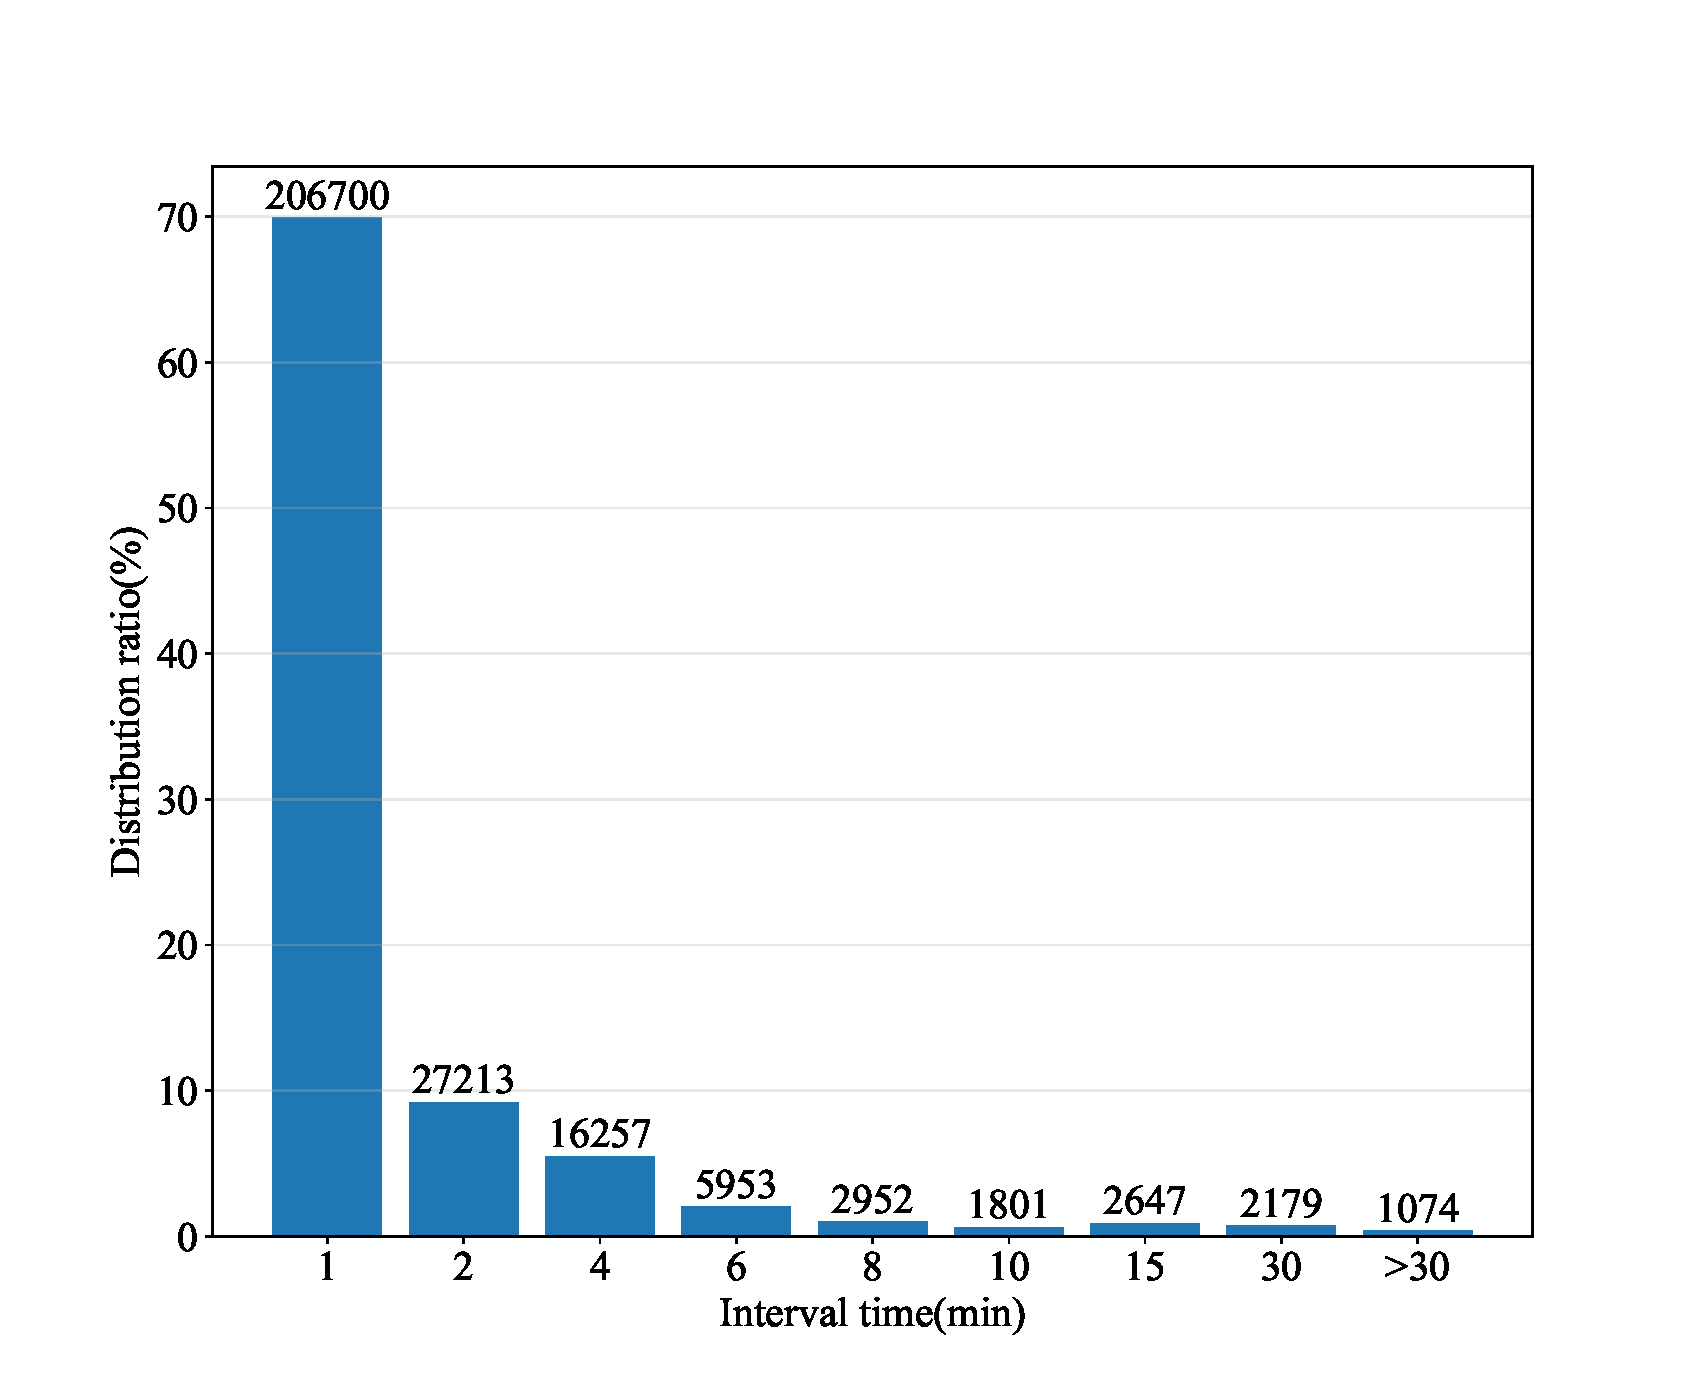
\includegraphics[scale=.35]{figs/Fig1.pdf}
	\caption{Time interval distribution of CEA-Curie-2011-2.1-cln workload.}
	\label{FIG:1}
\end{figure}

To address this problem, an efficient prediction model, referred to as online learning and k-nearest neighbors based (KNN-based) predictor with correction mechanism (OKCM), with low computational complexity and time overhead is proposed to predict job runtime for job scheduling. OKCM updates the model in real time through online learning with Huber loss function in low computational complexity and time overhead (less than $0.003s$ in our experiments). In addition, it is friendly to new users and users with a small amount of data through the KNN-based predictor, which is important for  real systems. The correction mechanism is designed to ensure safe execution of high-priority and subsequent jobs. 

To evaluate our model, we designed and implemented a trace-driven simulator, HPCsim, based on real job workloads. All simulated events and the related HPC environment including node resources, job scheduling, waiting queue, prioritizing policy, and backfilling mechanism are based on real workload traces and corresponding real HPC platform configurations. The results demonstrated that OKCM can achieve prediction accuracy of up to 82.3\% with a low overhead. Experiments further demonstrate that this model can achieve significant scheduling performance improvements, can be used to enhance the main prioritizing and backfilling methods, and is not limited to a certain type of scheduling.

The remainder of this paper is organized as follows: Section \ref{sect2} presents a review of the scheduling algorithm and closely related studies; Section \ref{sect3} presents the proposed model to predict job runtime; Section \ref{sect4} provides a demonstration of the accuracy of the proposed runtime prediction models and their scheduling performance; and Section \ref{sect5} presents the conclusions and potential future research.


\section{Related work} \label{sect2}
When a job arrives, the first step is to determine the priority of the job. The latest priority policy includes F1, F2, F3, F4 \cite{4SC17}, FAT, WFP1, WFP3, and UNICEF \cite{5Cluster09}. Without exception, the runtime of the job is one of the essential input parameter. 

To improve resource utilization, backfilling is currently the most common method in the scheduling system. Backfilling is a technique to improve resource utilization of HPC platforms by opportunistically running low-priority jobs when there are insufficient resources to run high-priority jobs \cite{11JSSPP}. In 1995, the seminal extensible Argonne scheduling system (EASY) backfilling algorithm \cite{12EASY} was developed and is now the de facto standard scheduling algorithm in many mainstream resource managers, such as Slurm \cite{13Slurm}, a well-known workload manager. Since then, many backfilling variants have been proposed, such as slack-based backfilling supporting priorities and bounded wait times \cite{14Prio}, or conservative backfilling, in which each waiting job is assigned a reservation \cite{15Utili}. To use backfilling, the scheduler must know the runtime of each job in advance for computing the reservation, to avoid delays in high-priority jobs. 

In practice, most job management systems ask the user to estimate the runtime. However, runtimes supplied by users are acknowledged to be inaccurate and overestimated \cite{11JSSPP}. Users unfamiliar with the HPC platform and their own jobs cannot provide precise runtimes. They tend to significantly overestimate runtimes to avoid job termination for exceeding the allotted runtime. User-requested runtimes also embody an inherently harmful backfilling trend. Users tend to request round runtimes (e.g., 1 h), resulting in 90\% of the jobs using the same ~20\% of runtime values \cite{6Tsafrir}, which limits the performance of backfilling in filling existing `holes' because many jobs appear the same.

For some time, several researchers believed that inaccurate runtimes had a positive effect on backfilling as they provided more flexibility and led to better scheduling performance. It was even proposed that runtimes should be randomized \cite{16Random}. In contrast, Tsafrir et al. \cite{6Tsafrir} demonstrated that precise knowledge of runtimes can have non-trivial effects on performance evaluation results. 

Considerable research has been conducted to improve the accuracy of job runtime estimates. Tsafrir et al.\citep{6Tsafrir} found that using historical information from the same user had a better predictive effect than ‘similar jobs’. However, using a historical average cannot effectively capture dynamic runtime changes such as periodic characteristics. Gaussier et al. \cite{2SC15} used a polynomial model to improve scheduling performance through a weighted asymmetric loss function. This method focused on the final performance, and the prediction was biased. Yuping Fan et al. \cite{3Cluster17} reported that many current prediction methods improve prediction accuracy at the expense of increasing underprediction. They adopted the Tobit model's censored regression capability to  keep a low underestimation rate. Ju-Won Park et al. \cite{9JSC} adopted support vector regression (SVRegression) to estimate runtime. McKenna et al. \cite{17Cluster16} compared runtimes predicted by decision tree, random forest, and k-nearest neighbors, and indicated that the decision tree can achieve the best results. Thonglek et al. \cite{18Cluster19} improved resource utility using long short-term memory (LSTM). Goshgar Ismayilov et al. \cite{24FGCS} used neural network based multi-objective evolutionary algorithm to improve scheduling. These studies and models focus only on improving accuracy, resulting in higher computational complexity and time overhead. They are difficult to deploy in a real-time scheduling system. Thus, an efficient prediction model that updates in real time and is friendly to new users is necessary.

\section{OKCM prediction model for job scheduling} \label{sect3}
\subsection{OKCM model}
The problem researched is to execute a set of parallel jobs with rigid requested resources on large-scale HPC systems represented by a set of $N_{max}$ homogeneous resources connected by interconnection topology. The jobs are submitted over time (online) to a centralized waiting queue. The job scheduler determines where and when to execute the jobs. Upon job completion, the system records the job along with a number of its attributes in the workload log. We define a \textit{workload} with the following data:
\begin{itemize} 
	\item The identification (ID) of the job $job_{id}$ 
	\item The ID of the user $user_{id}$ 
	\item Number of compute nodes required by the User $node_{req}$ 
	\item Requested time $t_{req}$ of the job by the user 
	\item Wait time $t_{wait}$ of the job (seconds)  
	\item Submit time of the job $t_{sub}$ (UTC timestamp, also known as release date and arrival time) 
	\item Number of allocated nodes by the system $node_{sys}$
	\item Real runtime $t_{real}$ of the job (seconds, only known after the job has been completed)
	\item Status $s$ (1 = ok, 0 = fail, 5 = cancel)
\end{itemize}

Although some workload logs have additional and more detailed information, such as I/O, memory, and compilation information, our model requires only the most basic information, available in most workload traces, to establish a job repository. The workload logs are a subset of the standard workload format (SWF) \cite{10JPDC}; thus, OKCM is applicable to a wide range of HPC platforms.

A high-level overview of OKCM is presented in Figure \ref{FIG:2}. Our time prediction model consists of two components, the prediction and correction mechanisms. Upon job arrival, OKCM retrieves job attributes from the repository. In the prediction mechanism, for users whose data accumulation is greater than the threshold (e.g., 25), online learning is used to predict the job runtime and update the model in real time. The KNN-based predictor is used for new users or users with less data than the threshold, which is important in a real system. During the job, effective runtime corrections are performed to guarantee safe execution of the job and ensure efficient scheduling of subsequent jobs.

\begin{figure}
	\centering
	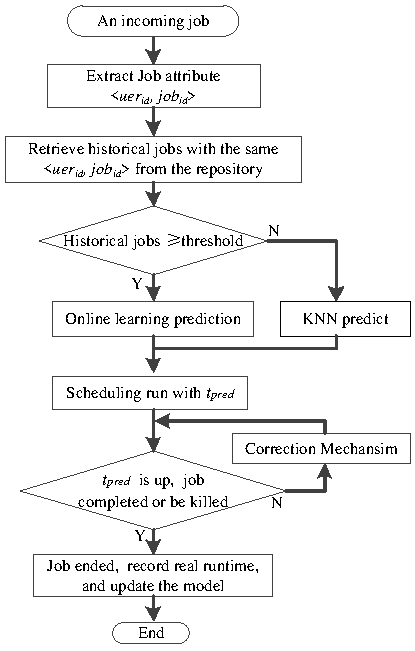
\includegraphics[scale=.75]{figs/Fig2.pdf}
	% pagewidth=70mm, pagehight=110mm
	\caption{OKCM runtime prediction model.}
	\label{FIG:2}
\end{figure}

\subsection{Prediction mechanism}
A \textit{job} is represented by a vector $x \in \mathbb{R}^{n} $ where $n$ is the number of features of the runtime prediction model, as shown in Table \ref{tbl1}. These features are recorded in the job repository. All features describe the status of users and jobs from multiple dimensions and are contained in four categories:
\begin{itemize} 
	\item Characteristics of the current job to be predicted, extracted from submit command (e.g., $node_{req}, t_{req}$). 
	\item Characteristics of user's job runtime, extracted from historical knowledge (e.g., $x_2, x_3, x_4, x_5, x_6, x_7, x_8$) 
	\item Characteristics of nodes requirement of the user (e.g., $x_9, x_{10}, x_{11}$)
	\item Characteristics of user behavior (e.g., $x_{12}, x_{13}, x_{14}$)
\end{itemize}

For users whose data accumulation is greater than the threshold, \textit{l2-regularized} online linear regression learning with the Huber loss function is proposed to provide predictions and perform updates in real time. The regression function is Equation \ref{equ1}:
\begin{equation} \label{equ1}
	f\left(w,x\right)=\sum_{i=0}^{n}w_ix_i \quad  w_i \in \mathbb{R}^n
\end{equation}

where $w_i$ are the parameters to be learned, and $x_i$ are the features of the \textit{job}.
\newcommand{\tabincell}[2]{\begin{tabular}{@{}#1@{}}#2\end{tabular}}

\begin{table}[width=.91\linewidth,cols=3,pos=h]
	\caption{Job features used for OKCM runtime prediction model.}\label{tbl1}
	\begin{center}
		% 当为0.91的时候,0.9+9.6+3.3	
		\begin{tabular*}{\tblwidth}{p{0.9cm} p{9.5cm} p{3.3cm}}
			\toprule
			Notation & Description & Meaning \\
			\midrule
			$x_0$ & number of compute nodes requested by the user $node_{req}$ & \multirow{2}{*}{\tabincell{l}{characteristics of job \\ to be predicted}}  \\
			$x_1$ & requested time of the user $t_{req}$ &   \\
			\hline
			$x_2$ & real runtime of the last job of the same user $t_{real}$, or $t_{req}$ if it is the first job & \multirow{7}{*} {\tabincell{l}{characteristics of user's\\ job runtime}}  \\
			$x_3$ & real runtime of the second-to-last job of the same user $t_{real2}$ &   \\
			$x_4$ & average real runtime of the last two jobs of the same user $A\!V\!G_{real2}$ &   \\
			$x_5$ & real runtime of the third-to-last job of the same user $t_{real3}$ &   \\
			$x_6$ & average real runtime of the last three jobs of the same user $A\!V\!G_{real3}$ &   \\
			$x_7$ & sum of historical real runtimes for all jobs of the same user $t_{all}$ &   \\
			$x_8$ & average historical real runtime for all jobs of the same user $A\!V\!G_{all}$ &   \\
			\hline
			$x_9$ & average historical requested nodes of the same user $node_{avgreq}$ & \multirow{3}{*}{\tabincell{l}{characteristics of nodes  \\ requirement of the user}}  \\
			$x_{10}$ & average historical  real nodes of the same user $node_{avgreal}$ &   \\
			$x_{11}$ & $node_{req}$ normalized by average resource request &   \\
			\hline
			$x_{12}$ & sin value of the submit time of the week $S\!I\!N_{week}$ &   \multirow{3}{*}{\tabincell{l}{characteristics of user \\ behavior}}  \\
			$x_{13}$ & sin value of the submit time of the day $S\!I\!N_{day}$ &   \\
			$x_{14}$ & time interval since last job ended of the same user $t_{interval}$ &   \\
			
			\bottomrule
		\end{tabular*}
	\end{center}
\end{table}

When training job runtime prediction model, the loss function is crucial. In workload files there are some abnormal jobs. Although their status is $‘ok’ (s = 1)$, they have particularly long or short runtimes. Therefor, the Huber loss function with \textit{l2-regularized} regression learning is suitable to reduce the effect of outliers on parameter estimation. In fact, the Huber loss function quadratically penalizes small errors to train efficiency, while the computation of absolute values of larger errors ensures regression robustness, as shown in Equation \ref{equ2}, where $\delta$ is a threshold.
\begin{equation} \label{equ2}
L\left(f\left(w,x\right),t_{real}\right)=\begin{cases}
\frac{1}{2}\left(f\left(w,x\right)-t_{real}\right)^2+\lambda\left \| w \right \|^2 & \left|f\left(w,x\right)-t_{real}\right|\leq \delta \\
\delta \left|f\left(w,x\right)-t_{real}\right|-\frac{1}{2}\delta^2+\lambda\left \| w \right \|^2 & otherwise
\end{cases}
\end{equation}

In scheduling systems, whether the model satisfies real-time requirements is an important factor affecting the practicality of the model. In OKCM, the Huber loss and a normalized adaptive online gradient algorithm \cite{19Norm} are combined to train the model. It is proved that regret bounds are dependent on the ratio of scales existing in the data rather than the absolute scale. The data do not need to be pre-normalized; the infer-time and infer-complexity are reduced, and the algorithms are more robust. This is important for the scheduling system.

Compared to adaptive learning, when training, if the new features are larger than the previous ones, the weights are updated by the vector element $s_i$ which stores the magnitude of feature $i$ according to $s_i=max\left|x_i\right|$. A gradient descent is performed according to Equation \ref{equ3}.
\begin{equation} \label{equ3}
w_i=w_i-\eta\sqrt{\frac{t}{N}}\frac{1}{s_i\sqrt{G_i}}\frac{\partial{L\left (f\left(w,x\right),t_{real}\right)}}{\partial{w_i}}
\end{equation}
where,
\begin{equation}
N=N+\sum_{i}\frac{x_i^2}{s_i^2}
\end{equation}
\begin{equation}
G_i=G_i+\left(\frac{\partial{L\left (f\left(w,x\right),t_{real}\right)}}{\partial{w_i}}\right)^2
\end{equation}

Using $N$ causes the learning rate to control the average change in prediction from an update. Using $G$ completes the adaptive gradient descent.

For new users or users with a small data accumulation, several machine learning algorithms, such as SVRegressor and light gradient boosting machine regressor (LGBMRegressor), which need huge amounts of data to learn, are unsuitable because of this inherent flaw in the algorithms. In our model, this problem is addressed using the KNN-based predictor. As shown in Figure \ref{FIG:3}, the overall runtime is bounded, and part of the time period is stepped. The running time of similar jobs in some time periods is similar. The lazy learning KNN is a simple but effective method to predict the runtime in job scheduling, shown as Algorithm \ref{alg1}. Only the runtime of the first job is set as $t_{req}$. The runtime of the second job is set as the first job runtime $t_{first}$. If the completed job number $2\leq num \le$  \textit{threshold}, the $t_{pred}$ is learned by the KNN-based predictor. 
\begin{figure}
	\centering
	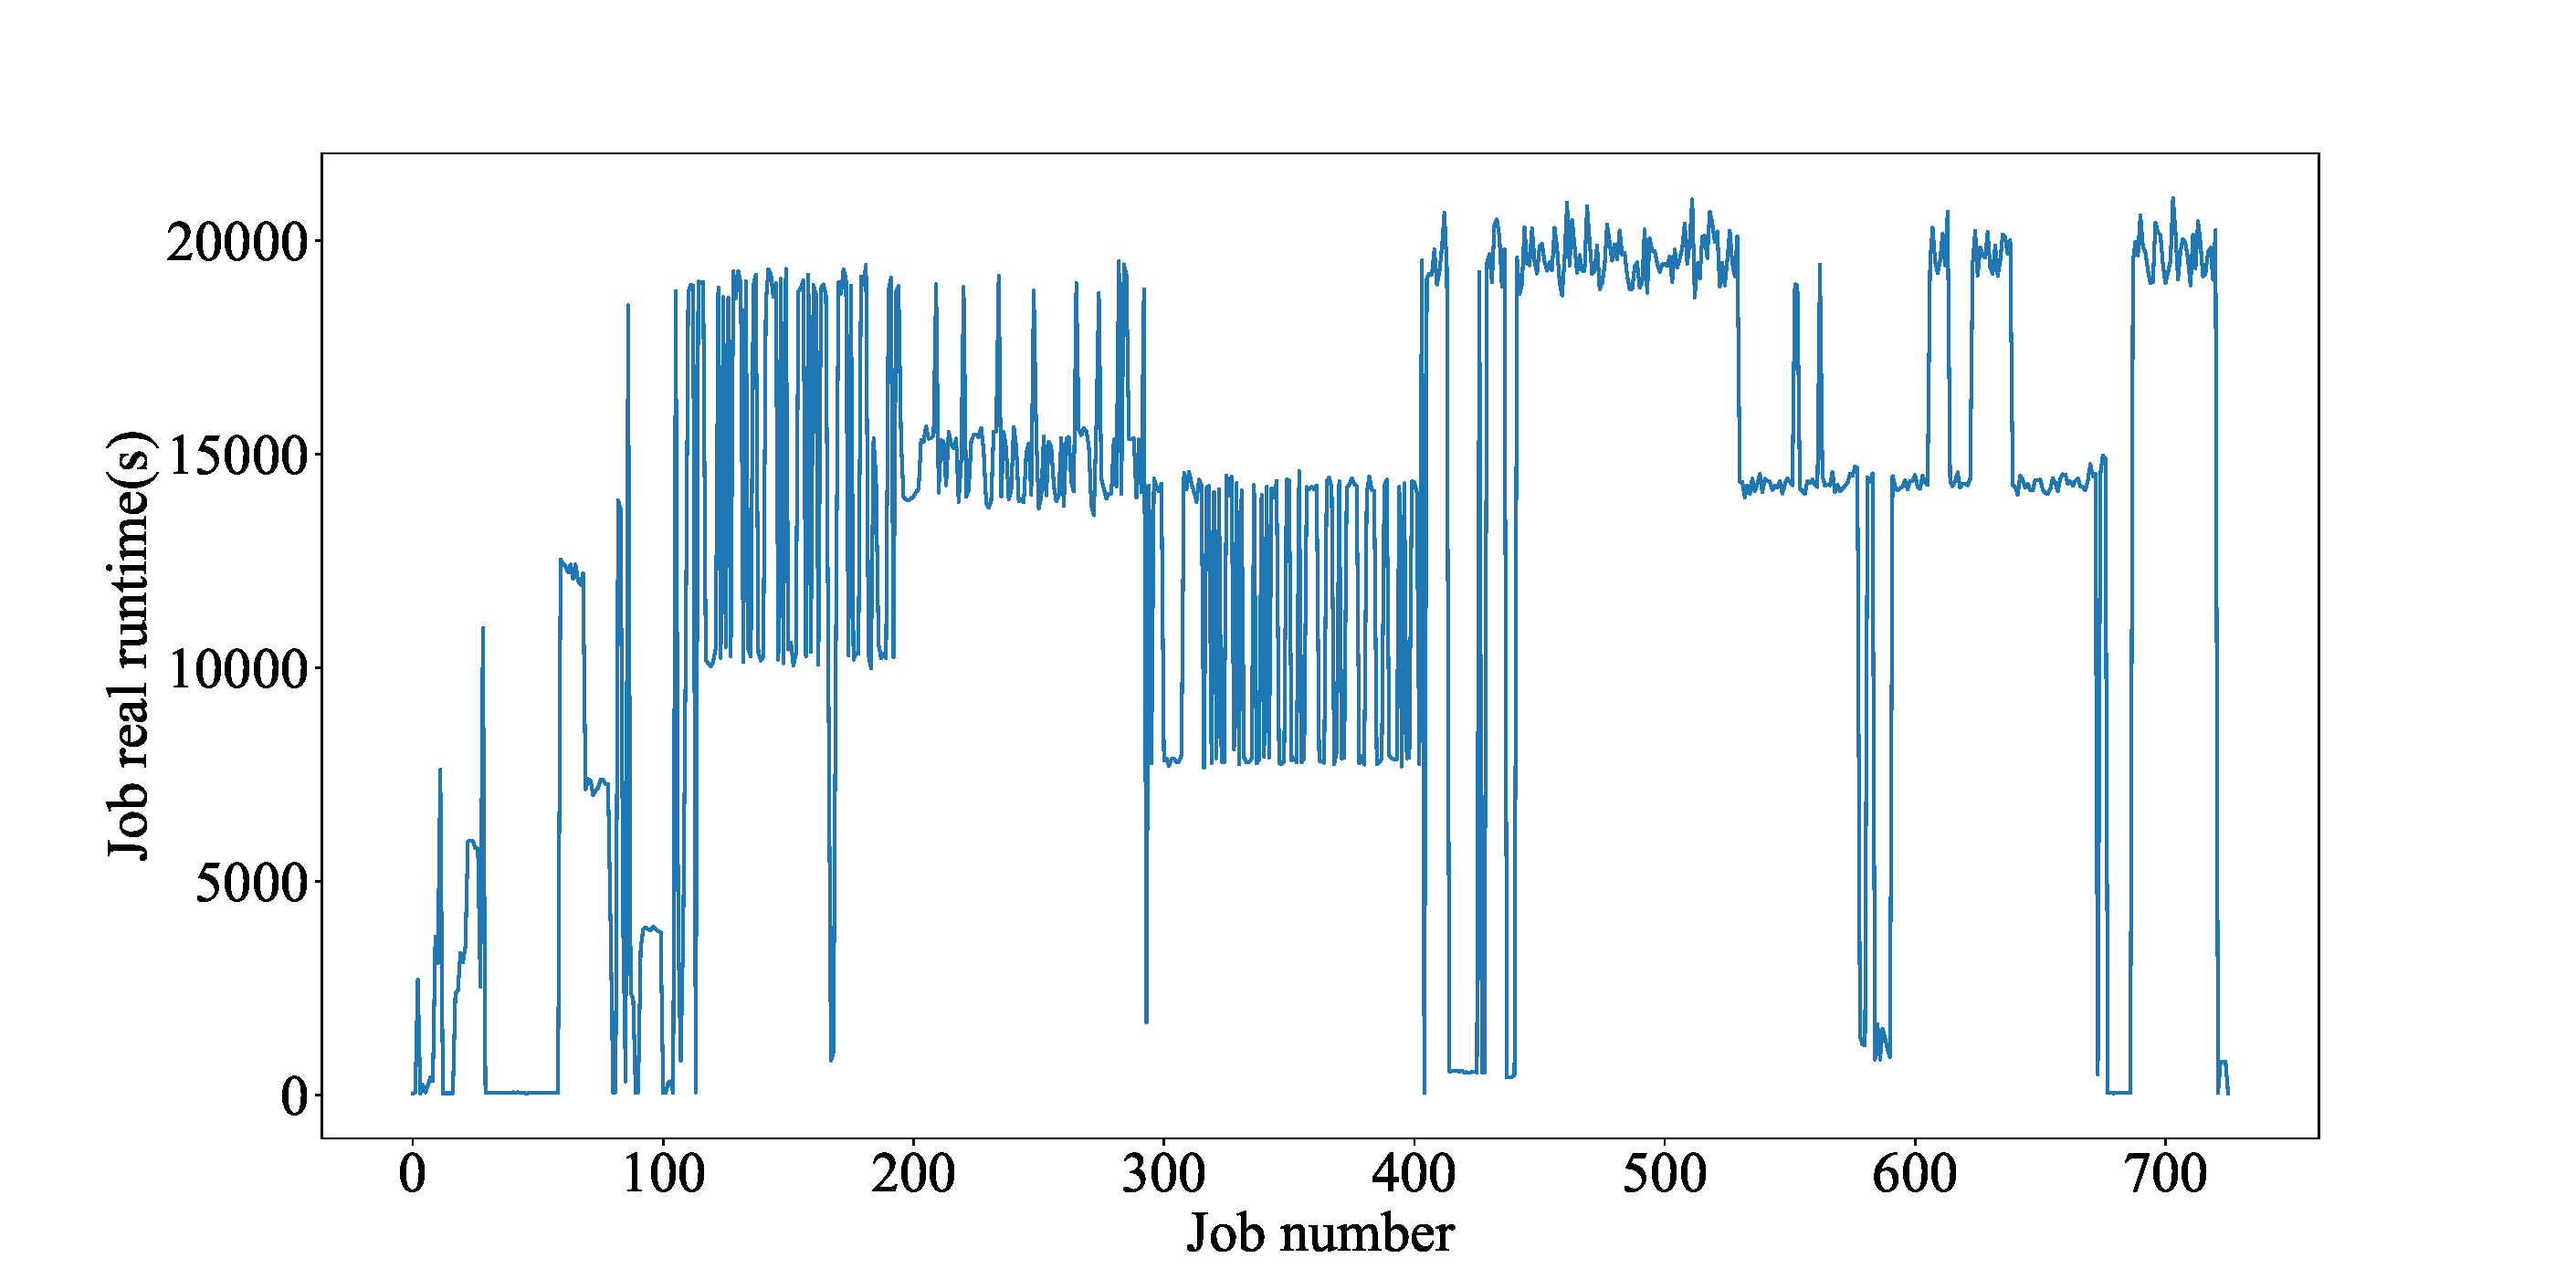
\includegraphics[scale=.30]{figs/Fig3.pdf}
	\caption{Real job runtime in ANL-Intrepid-2009-1 workload of user 176.}
	\label{FIG:3}
\end{figure}

\floatname{algorithm}{Algorithm}  
\renewcommand{\algorithmicrequire}{\textbf{Input:}}  
\renewcommand{\algorithmicensure}{\textbf{Output:}}  

\begin{algorithm}  
	\caption{KNN-based predictor}  \label{alg1}
	\begin{algorithmic}[1] %show the line number
		\Require $Features \left<x_0^j, x_1^j, x_{13}^j\right>$ of all arrived job $num$ extracted from job reposity
		\Ensure $t_{pred}$ the predicted time of the job  
		\If {the new arriving job $job_{num}<$ \textit{threshold} for the same user}  
		\State Normalize all the features by its corresponding dimension $x_i=\frac{x_i-\bar{x}_i}{s_i}$ 
		\State $D^j$ $\gets$ normalized Euclidean distance $\sum_{i=0}^{num}\left(x_i-x_i^j\right)^2$ 
		\State Sort select the K neighbors by $D^j$ and $t_sub$   
		\State $t_{pred} \gets $ the median runtime of the K neighbors
		\EndIf  
	\end{algorithmic}  
\end{algorithm}  

where, $\bar{x}_i=\frac{1}{n}\sum_{j=0}^{num}x_i^j$ and $s_i=\sqrt{\frac{1}{n-1}\sum_{j=0}^{num}\left(x_i-\bar{x}_i\right)^2}$ represent expected value and standard deviation, respectively. Features of the KNN-based predictor are a subset of the previous features, because in the same user space, the three features are able to characterize the similarity of jobs through normalized Euclidean distance. If the Euclidean distances are the same, the closest in time are k-nearest neighbors.

\subsection{Correction mechanism}

When predicting, the model may predict longer than the actual runtime (overprediction) or shorter than the actual runtime (underprediction). Overprediction is manageable, as it does not affect the running of the job. However, underprediction leads to unfinished jobs that must continue to run past the allotted runtime. For a deadline-constrained system, underprediction is technically unacceptable. Users do not tolerate their jobs being prematurely terminated simply because the model predicted a shorter runtime than the actual runtime. 

For underprediction, Tsafrir et al. \cite{6Tsafrir} increased post-estimate predictions in a gradual manner. The first adjustment adds only one minute to the prediction. If this is not sufficient, the $i^{th}$ prediction correction adds $15\times2^{i-2}$ min (15 min, 30 min, 1 h, 2 h, etc.), as shown in Figure \ref{FIG:4}. Such a method may allow more jobs to be backfilled, which may cause long wait times for high-priority jobs. 
\begin{figure}
	\centering
	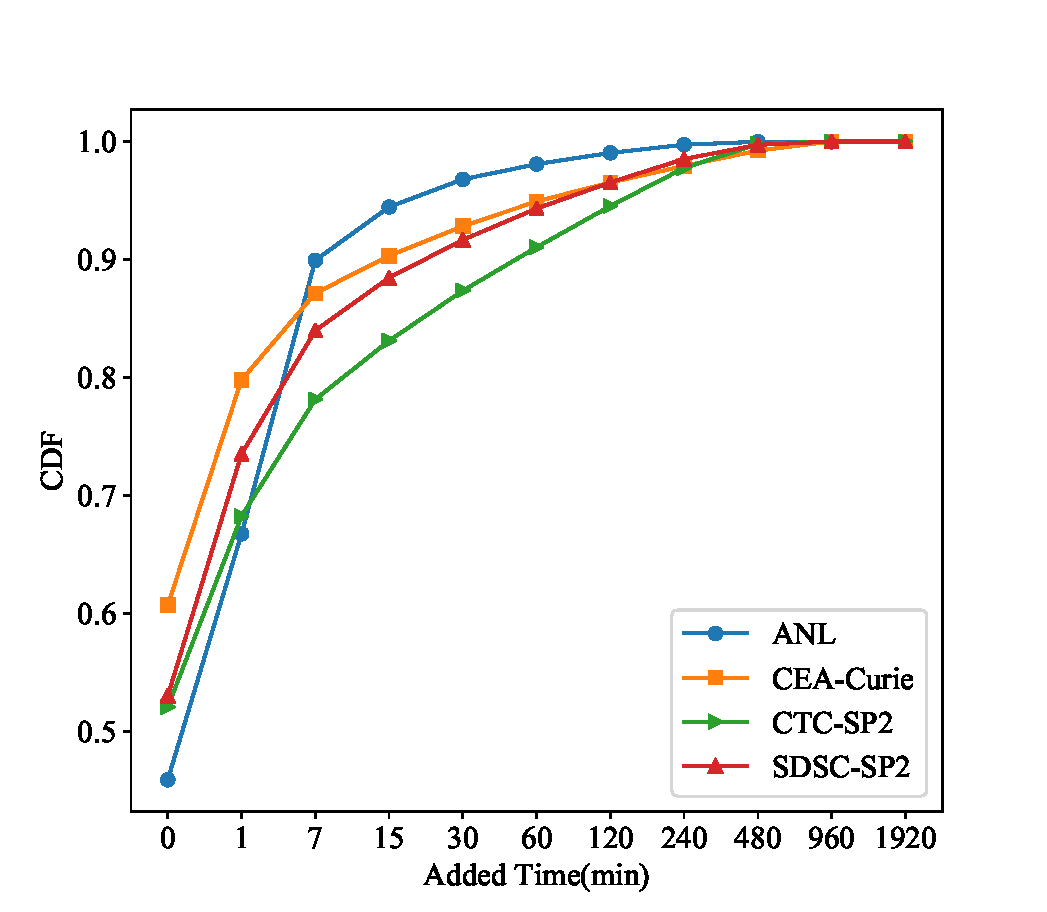
\includegraphics[scale=.43]{figs/Fig4.pdf}
	\caption{CFD result of incremental correction mechanism.}
	\label{FIG:4}
\end{figure}

A checkpoint-based scheduling algorithm is used to solve such  problem \cite{20Check}. Jobs are checkpointed and terminated until the highest-priority job receives its requested resources. The checkpointed jobs are placed at the head of the queue to facilitate continued execution. However, this method requires additional system support.

Our model directly corrects the runtime to user-requested runtime.  OKCM already has a high prediction accuracy, direct correction to the requested time can ensure the safe run of high-priority and subsequent jobs. The user-requested time serves as a kill-time. Correspondingly, the predicted time is only for the prioritizing policies and backfilling mechanism. Once the prediction is corrected, the model updates the remaining time and extra nodes to make new backfilling reservations. 

\subsection{HPCsim system}
To evaluate the scheduling performance, HPCsim, a trace-driven simulator, was designed and implemented based on real system workload inputs.

All simulated events and the related HPC environment including node resources, job scheduling, job queue, prioritizing policy, and backfilling mechanism are based on real workload traces and corresponding real HPC platform configurations \cite{10JPDC}. Prioritizing policies including F1, F2, F3, F4 \cite{4SC17}, FAT, WFP1, WFP3, and UNICEF \cite{5Cluster09} are implemented in our scheduling system. The aggressive backfilling algorithm is optional with these priority policies. When using the backfilling option, jobs are sorted by priority, and the aggressive backfilling algorithm checks if low-priority jobs can be executed without delaying the highest priority jobs. All scheduling actions can be performed over the user-requested and predicted time. Upon a job termination, including a normal completion, the end of the predicted time, or a job being killed, the scheduler is notified to correct runtime or  schedule other queued jobs on free nodes. SimGrid-3.25 \cite{21JPDC} is used to realistically simulate the HPC environment and operation of HPC jobs with multiple nodes, computing speed, and network topology.

\section{Experiment and analysis} \label{sect4}
\subsection{Experiment scheme}
Based on the simulator proposed in this study, a comprehensive verification scheme is designed, including prediction accuracy and scheduling performance. To ensure the validity of the accuracy test, walk-forward validation is used. When a job arrives, the current model is used to make a prediction. Once the actual runtime is known after the job is completed, the model is updated immediately for predicting the next job. This mimics a real-world job scheduling scenario. To test the scheduling performance, each workload is sampled without replacement seven times, each time for 30 consecutive days. The median and mean values of average bounded slowdown and average waiting time are recorded and analyzed.

We analyzed four real workload traces collected from real HPC systems from the Parallel Workload Archive \cite{10JPDC}, including ANL-Intrepid-2009-1, CEA-Curie-2011-2.1-cln, CTC-SP2-1996-3.1-cln, and SDSC-SP2-1998-4.2-cln, as listed in Table \ref{tbl2}. These traces are very representative, with configurations ranging from 128 to 163,840 nodes, jobs number from 73,496 to 321,826, and measurement dates from 1996 to 2011.
\begin{table}[width=.71\linewidth,cols=6,pos=h]
	\caption{Real workload traces used for evaluating runtime prediction and scheduling.}\label{tbl2}
	\begin{tabular*}{\tblwidth}{@{} LLLLLL@{} }
		\toprule
		Name & Nodes & Job Tatal & Test Job range & Year & During\\
		\midrule
		CEA-Curie-2011-2.1-cln & 93,321 & 321,826 & 6,099-10,546 & 2011 & 20\\
		ANL-Intrepid-2009-1 & 163,840 & 68,936 & 10,152-40,956 & 2009 & 8\\
		CTC-SP2-1996-3.1-cln & 338 & 77 ,222 & 5,985-8,391 & 1997 & 11\\
		SDSC-SP2-1998-4.2-cln & 128 & 73,496 & 2,189-3,523 & 1996 & 23\\
		\bottomrule
	\end{tabular*}
\end{table}
\subsection{Prediction accuracy}
The prediction accuracy is the ratio of $t_{real}$ to $t_{pred}$, as shown in Equation \ref{equ6}.
\begin{equation} \label{equ6}
accurancy=\begin{cases}
1 & t_{real} = t_{pred} \\
t_{pred}/t_{real} & t_{real} \ge t_{pred} \\
t_{real} / t_{pred} & t_{real} \le t_{pred}
\end{cases}
\end{equation}

where $t_{real}$ is the real runtime and $t_{pred}$ is the predicted time by our model. An accuracy of 1.00 represents 100\% accuracy. 
\begin{figure}[htbp] 
	\centering	
	\subfigure[CEA-Curie-2011-2.1-cln workload]{
		\begin{minipage}[t]{0.45\linewidth}
			\centering
			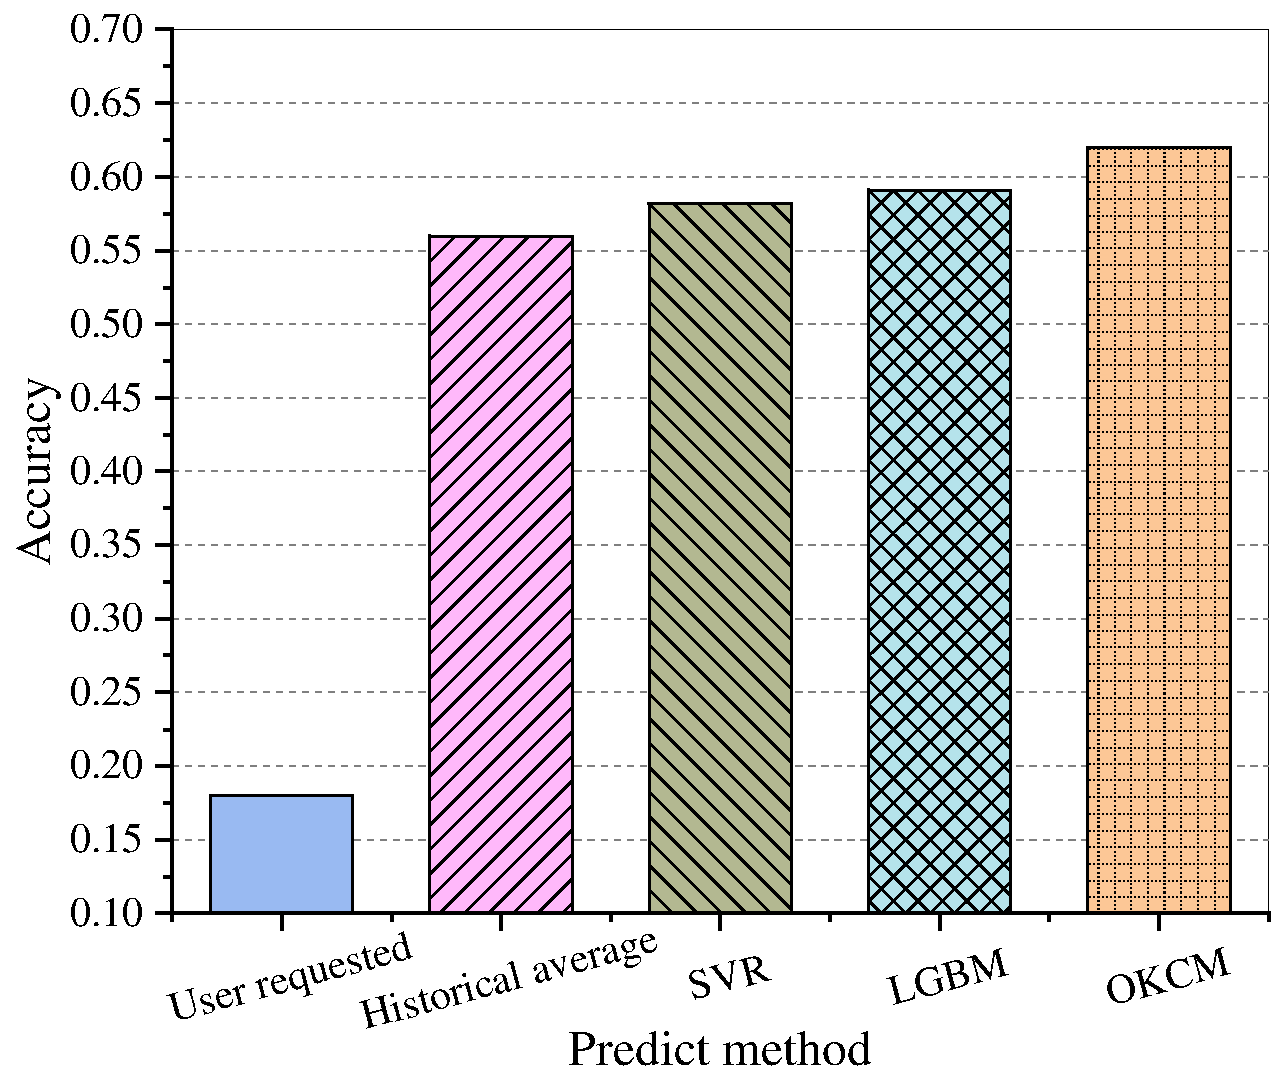
\includegraphics[scale=.34]{figs/Fig5a.pdf}
			%\caption{fig1}
		\end{minipage}%
	}%
	\subfigure[ANL-Intrepid-2009-1 workload]{
		\begin{minipage}[t]{0.45\linewidth}
			\centering
			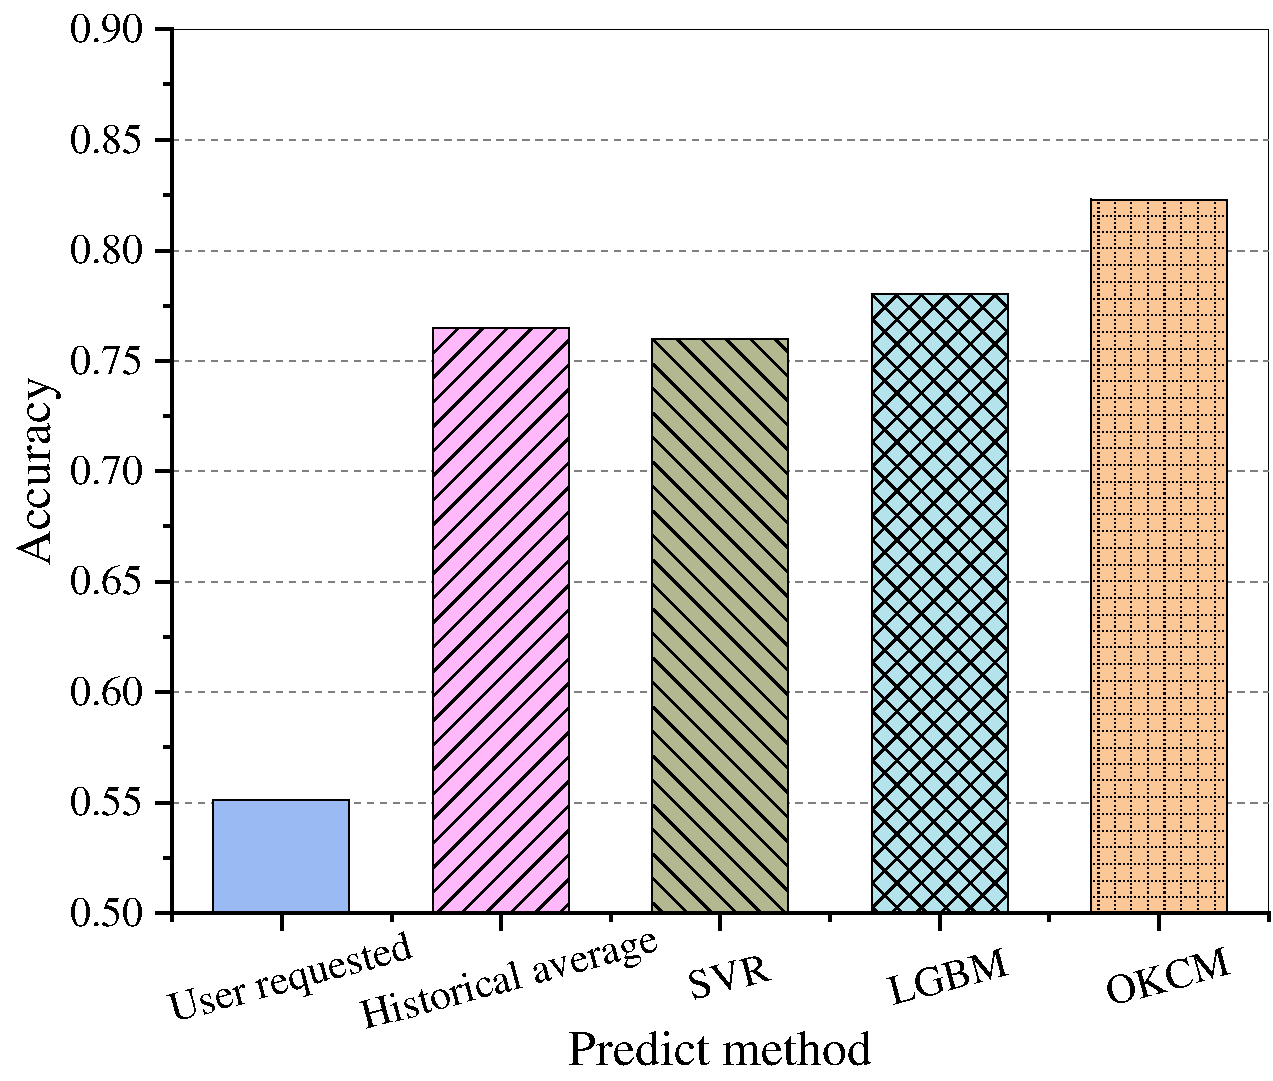
\includegraphics[scale=.34]{figs/Fig5b.pdf}
			%\caption{fig2}
		\end{minipage}%
	}%
	\, %这个回车键很重要 \quad也可以
	\subfigure[CTC-SP2-1996-3.1-cln workload]{
		\begin{minipage}[t]{0.45\linewidth}
			\centering
			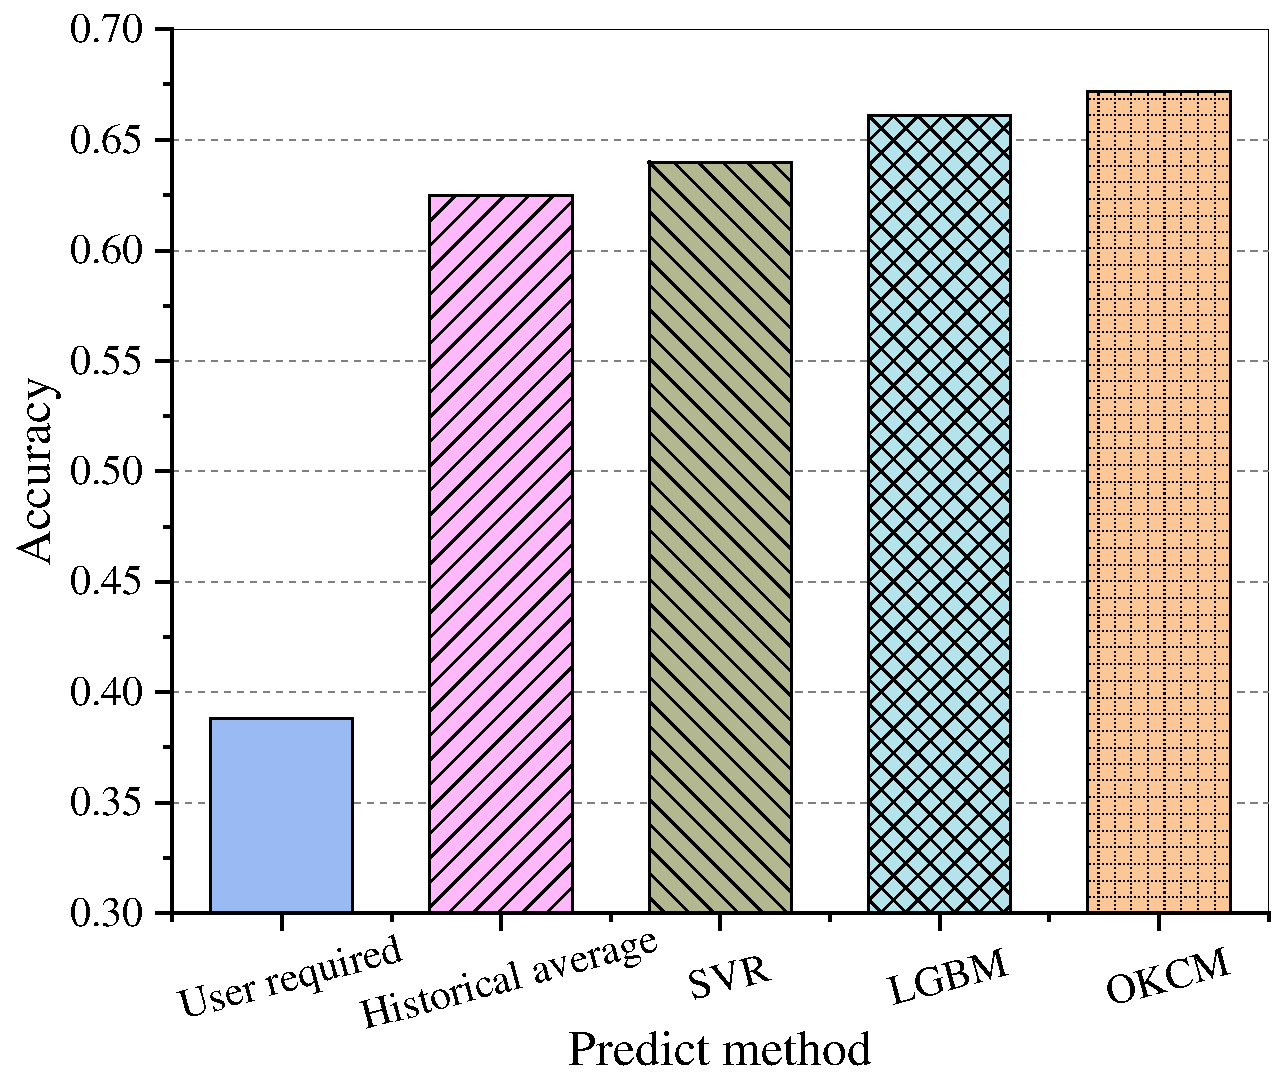
\includegraphics[scale=.34]{figs/Fig5c.pdf}
			%\caption{fig2}
		\end{minipage}
	}%
	\subfigure[SDSC-SP2-1998-4.2-cln workload]{
		\begin{minipage}[t]{0.45\linewidth}
			\centering
			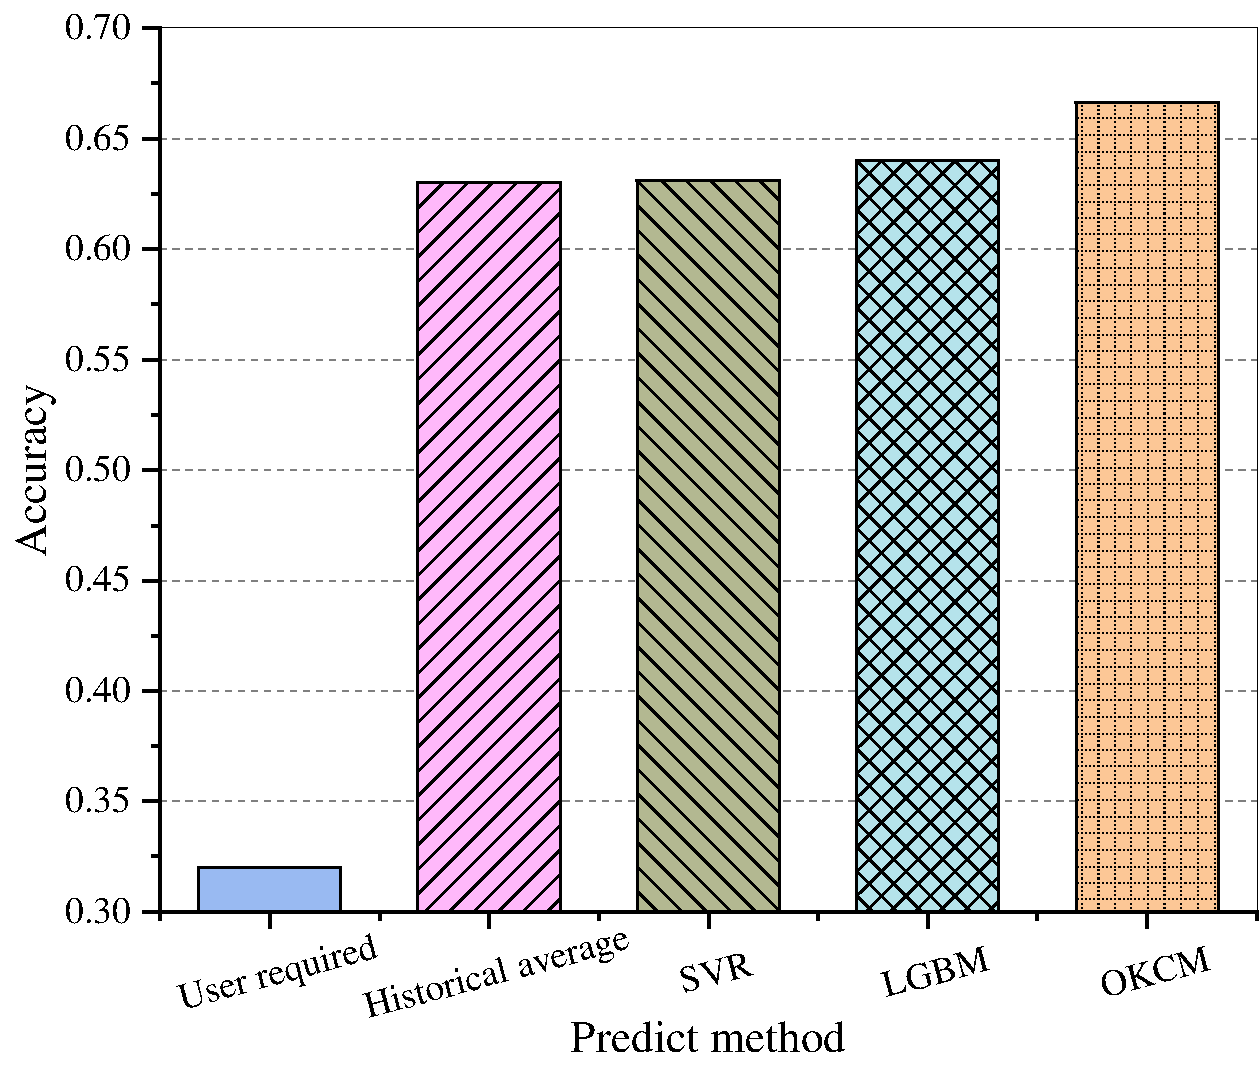
\includegraphics[scale=.34]{figs/Fig5d.pdf}
			%\caption{fig2}
		\end{minipage}
	}%
	
	\centering
	\caption{Comparison of runtime prediction accuracy of different algorithm.} \label{FIG:5}
\end{figure}
Figure \ref{FIG:5} shows the prediction results of different algorithms. It is observed that the OKCM model achieved the best prediction accuracy on all workloads. The accuracy is 82.3\% in ANL-Intrepid, 67.1\% in CTC-SP2, 66.3\% in SDSC-SP2, and 62.1\% in CEA-Curie. OKCM prediction is 1.45-3.44 times more accurate than user-requested time. Compared with SVRegressor and LGBMRegressor algorithms, OKCM achieves a 3.3\%-6.3\% performance improvement.

\subsection{Scheduling performance}
\begin{figure}
	% Fig5 weight 209mm, height 190mm for visio
	\centering
	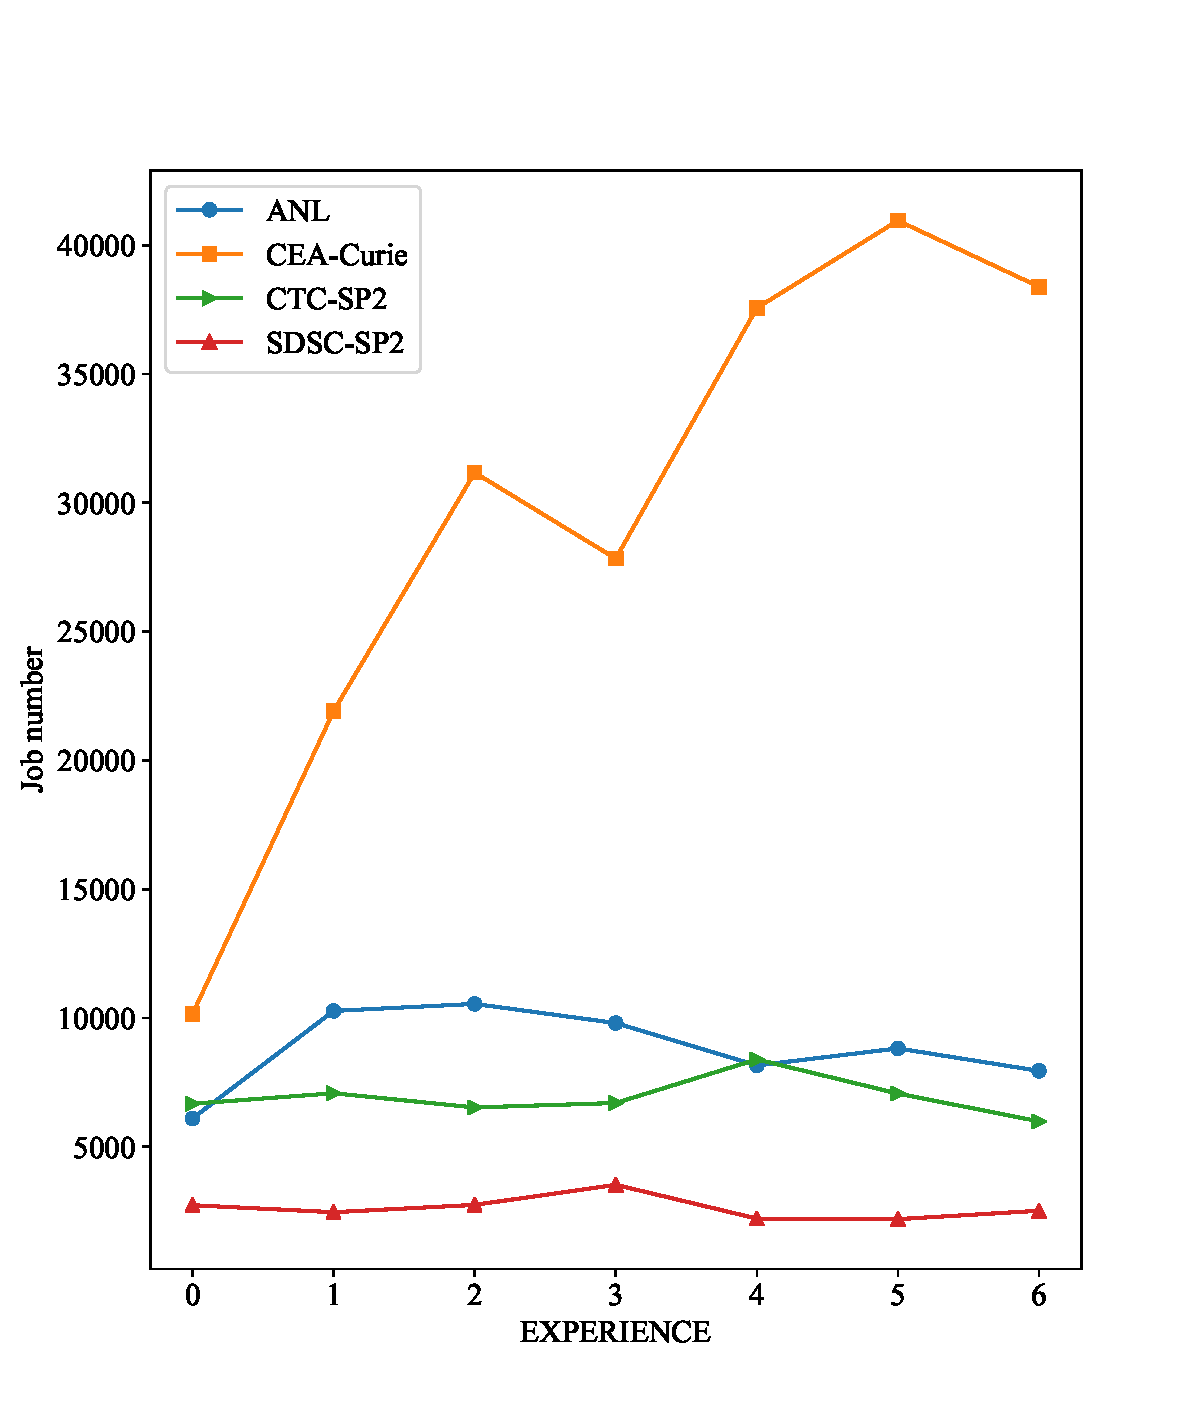
\includegraphics[scale=.43]{figs/Fig6.pdf}
	\caption{Job numbers for scheduling of each workload.}
	\label{FIG:6}
\end{figure}
Figure \ref{FIG:6} shows the number of jobs scheduled for each workload. The performance is measured by the average bounded slowdown ($A\!V\!Gblsd$) and average waiting time ($A\!V\!Gwt$).

The $blsd$ slowdown of a job is the ratio of job response time to its actual runtime, which is defined as shown in Equation \ref{equ7}:
\begin{equation} \label{equ7}
blsd^j=max\left(\frac{t_{wait}^{j}+t_{real}^{j}}{max\left(t_{real}^{j},\tau\right)},1\right)
\end{equation}

where $t_{wait}^{j}$ is the waiting time of job $j$ and $\tau$ is a constant preventing overemphasis of the importance of extremely short jobs. In previous studies, $\tau$ has generally been set to 10 s. The $A\!V\!Gblsd$ of $M$ total jobs is defined as shown in Equation \ref{equ8}:
\begin{equation} \label{equ8}
A\!V\!Gblsd=\frac{1}{M}\sum_{j}max\left(\frac{t_{wait}^{j}+t_{real}^{j}}{max\left(t_{real}^{j},\tau\right)},1\right)
\end{equation}

$A\!V\!Gwt$ measures quality of service by the waiting time of $M$ total jobs, defined as Equation \ref{equ9}.
\begin{equation} \label{equ9}
A\!V\!Gwt=\frac{1}{M}\sum_{j}t_{wait}^j
\end{equation}

The box-whisker plot is used to illustrate the scheduling performance in Figures \ref{Fig:7}-\ref{Fig:10}. The orange line shows the median value, the box shows the $25^{th}-75^{th}$ percentile values, and the red point is the mean of the data. In these figures, (a) shows the box plot of $A\!V\!Gblsd$ using user-requested time, (b) illustrates $A\!V\!Gblsd$ of OKCM predicted time, (c) and (d) show the result of $A\!V\!Gwt$ with user-requested time and OKCM predicted time, respectively.

\subsubsection{CEA-Curie scheduling performance}
\begin{figure}[htbp] 
	\centering	
	\subfigure[$A\!V\!Gblsd$ with user-requested time]{
		\begin{minipage}[t]{0.44\linewidth}
			\centering
			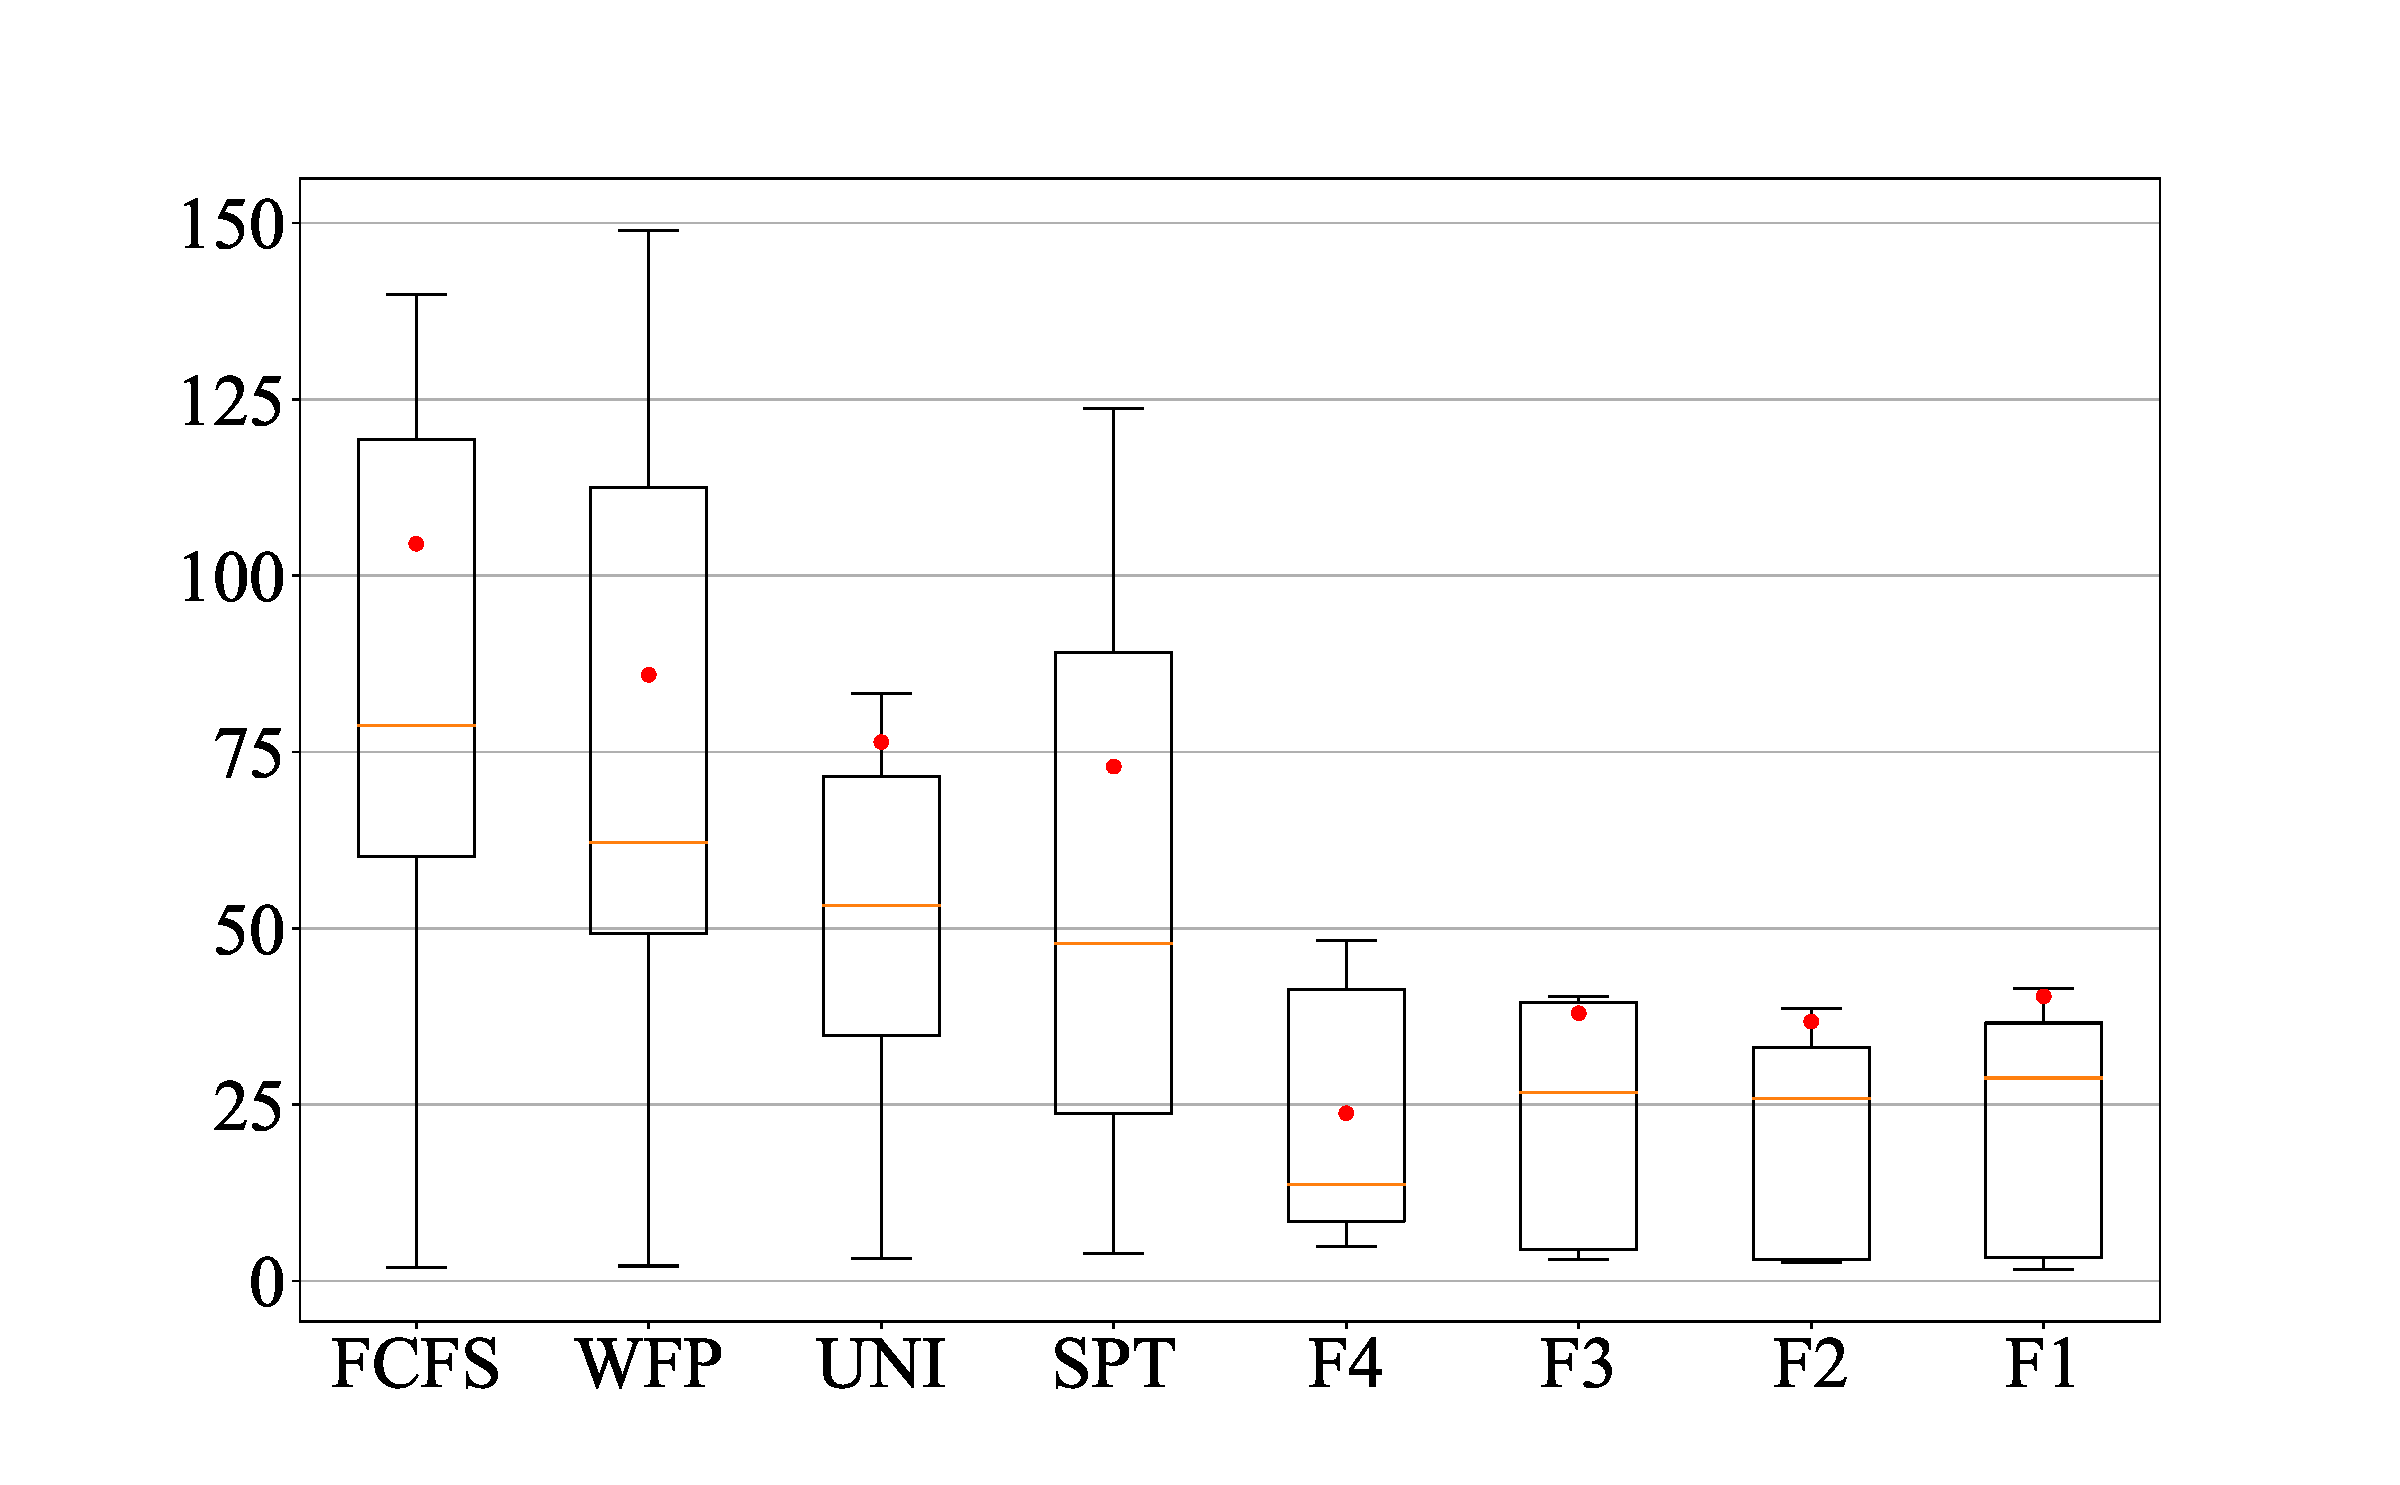
\includegraphics[scale=.20]{figs/Fig7a.pdf}
			%\caption{fig1}
		\end{minipage}%
	}%
	\subfigure[$A\!V\!Gblsd$ with predicted time]{
		\begin{minipage}[t]{0.44\linewidth}
			\centering
			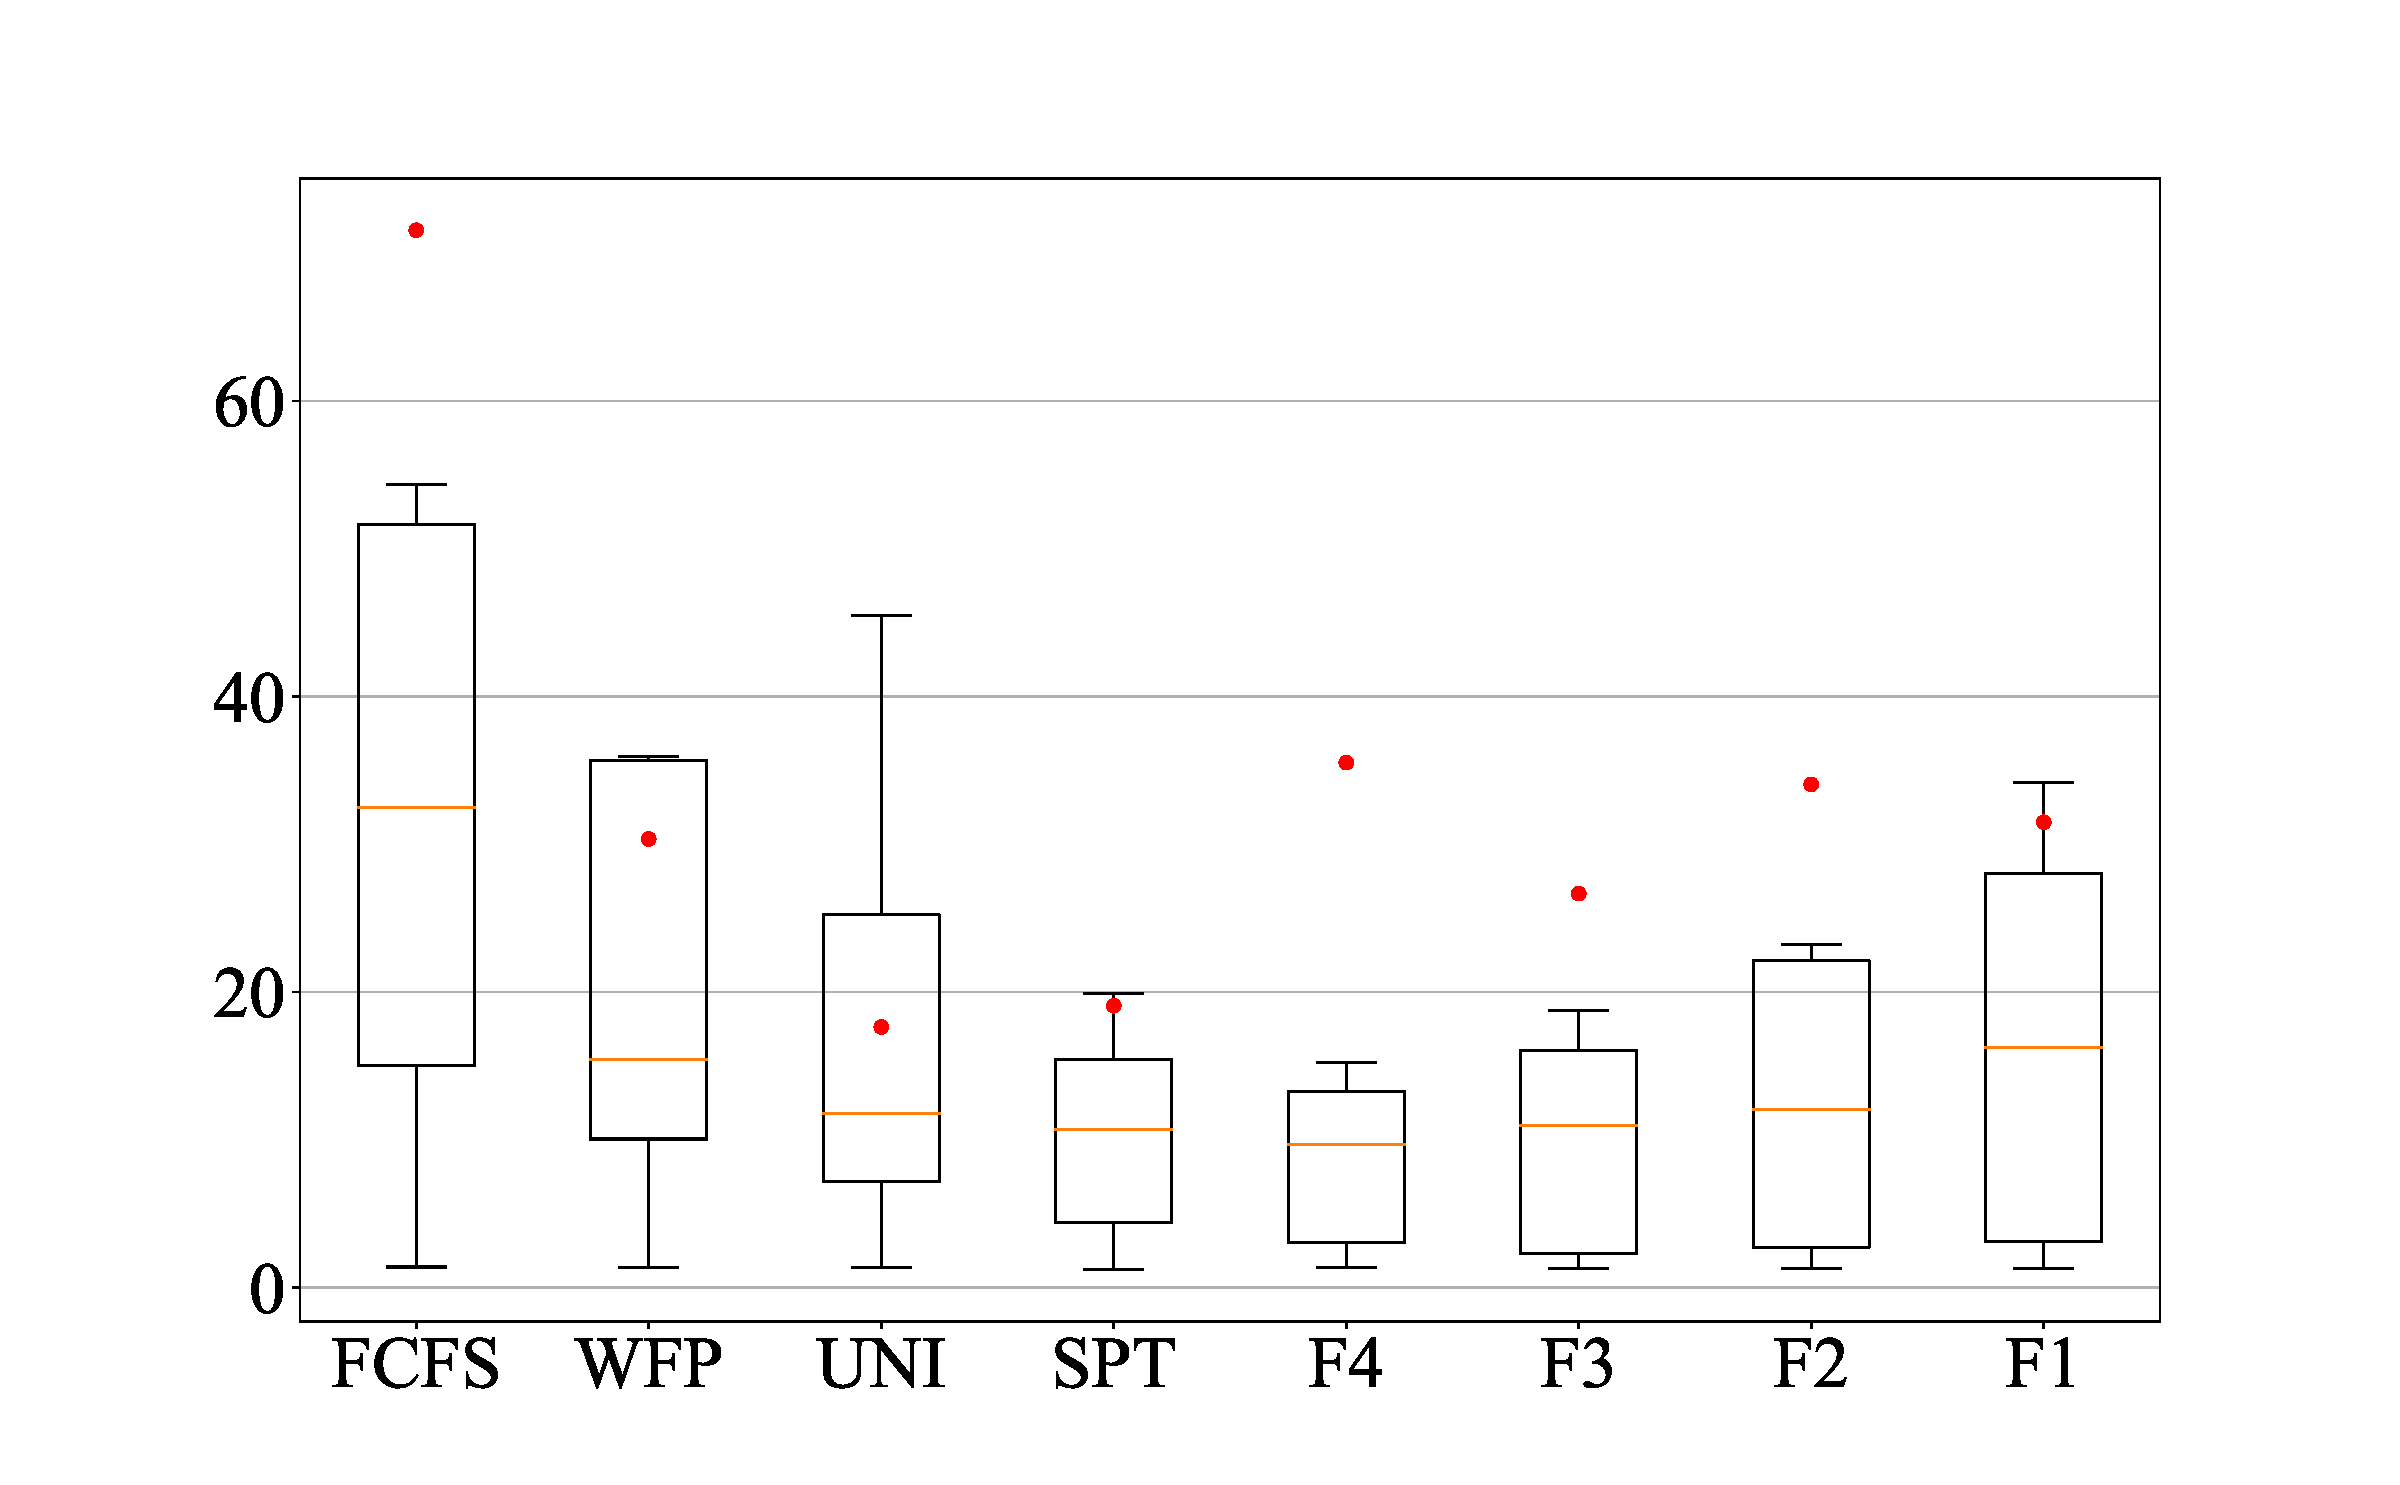
\includegraphics[scale=.20]{figs/Fig7b.pdf}
			%\caption{fig2}
		\end{minipage}%
	}%
	\, %这个回车键很重要 \quad也可以
	\subfigure[$A\!V\!Gwt$ with user-requested time]{
		\begin{minipage}[t]{0.44\linewidth}
			\centering
			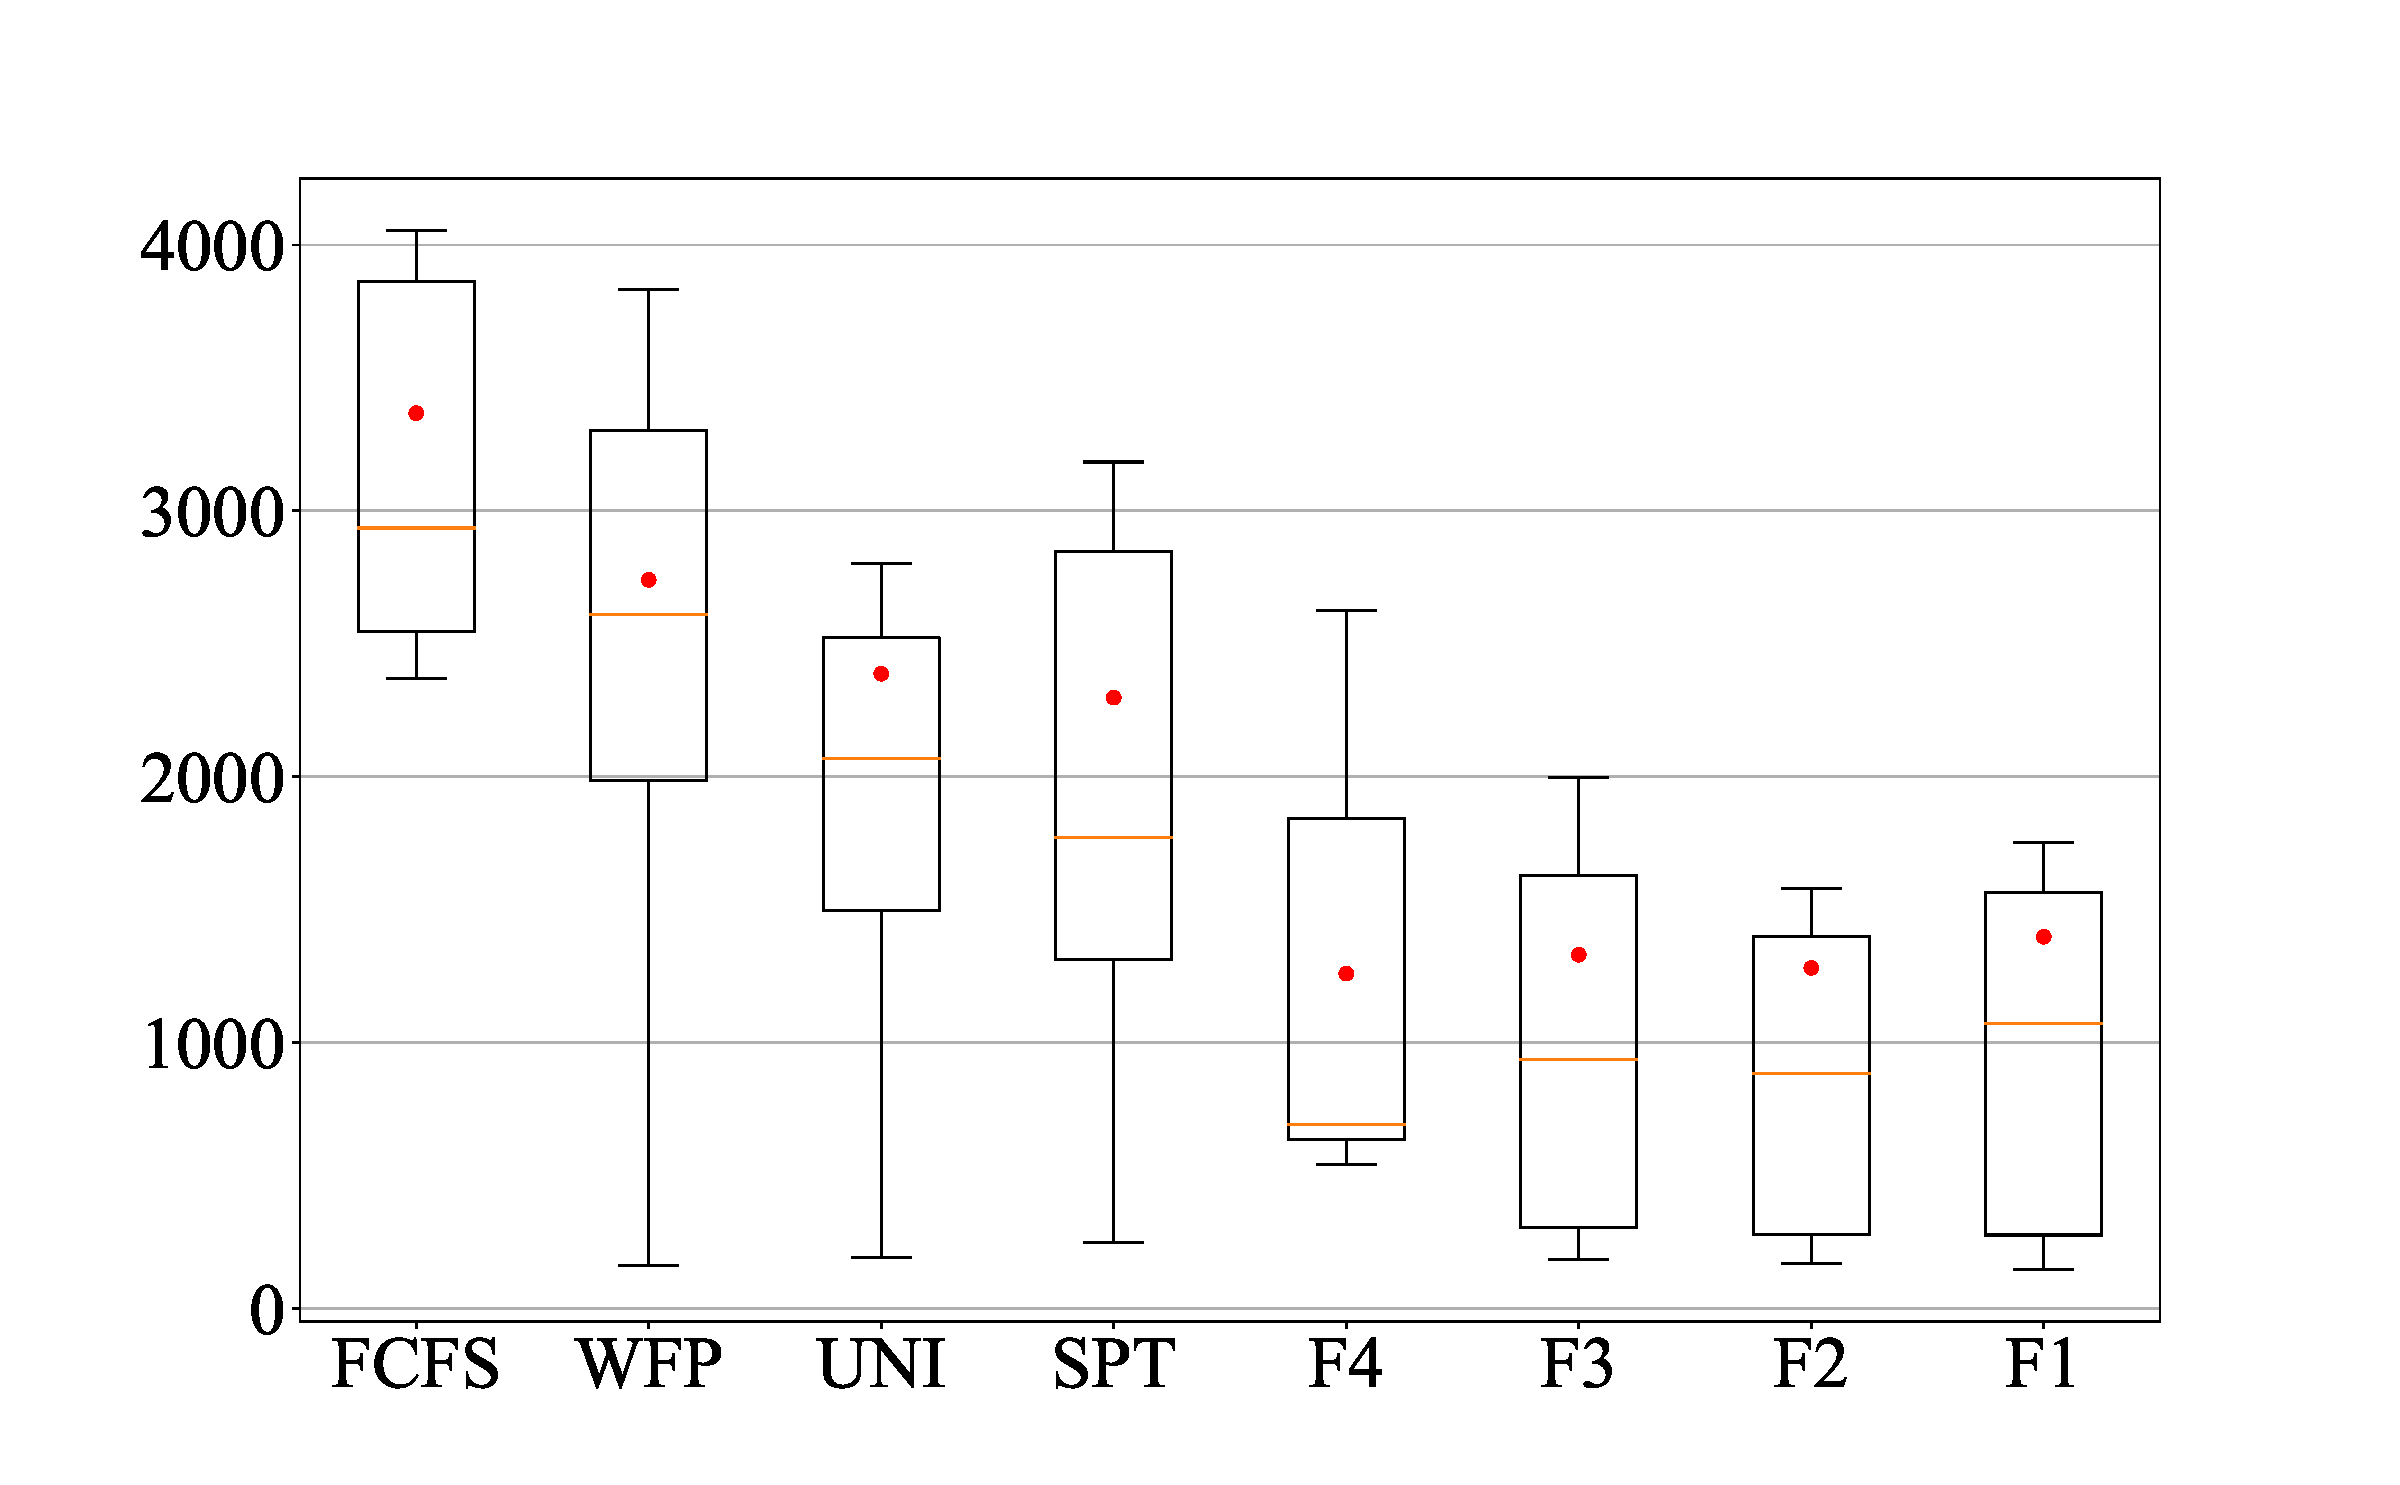
\includegraphics[scale=.20]{figs/Fig7c.pdf}
			%\caption{fig2}
		\end{minipage}
	}%
	\subfigure[$A\!V\!Gwt$ with predicted time]{
		\begin{minipage}[t]{0.44\linewidth}
			\centering
			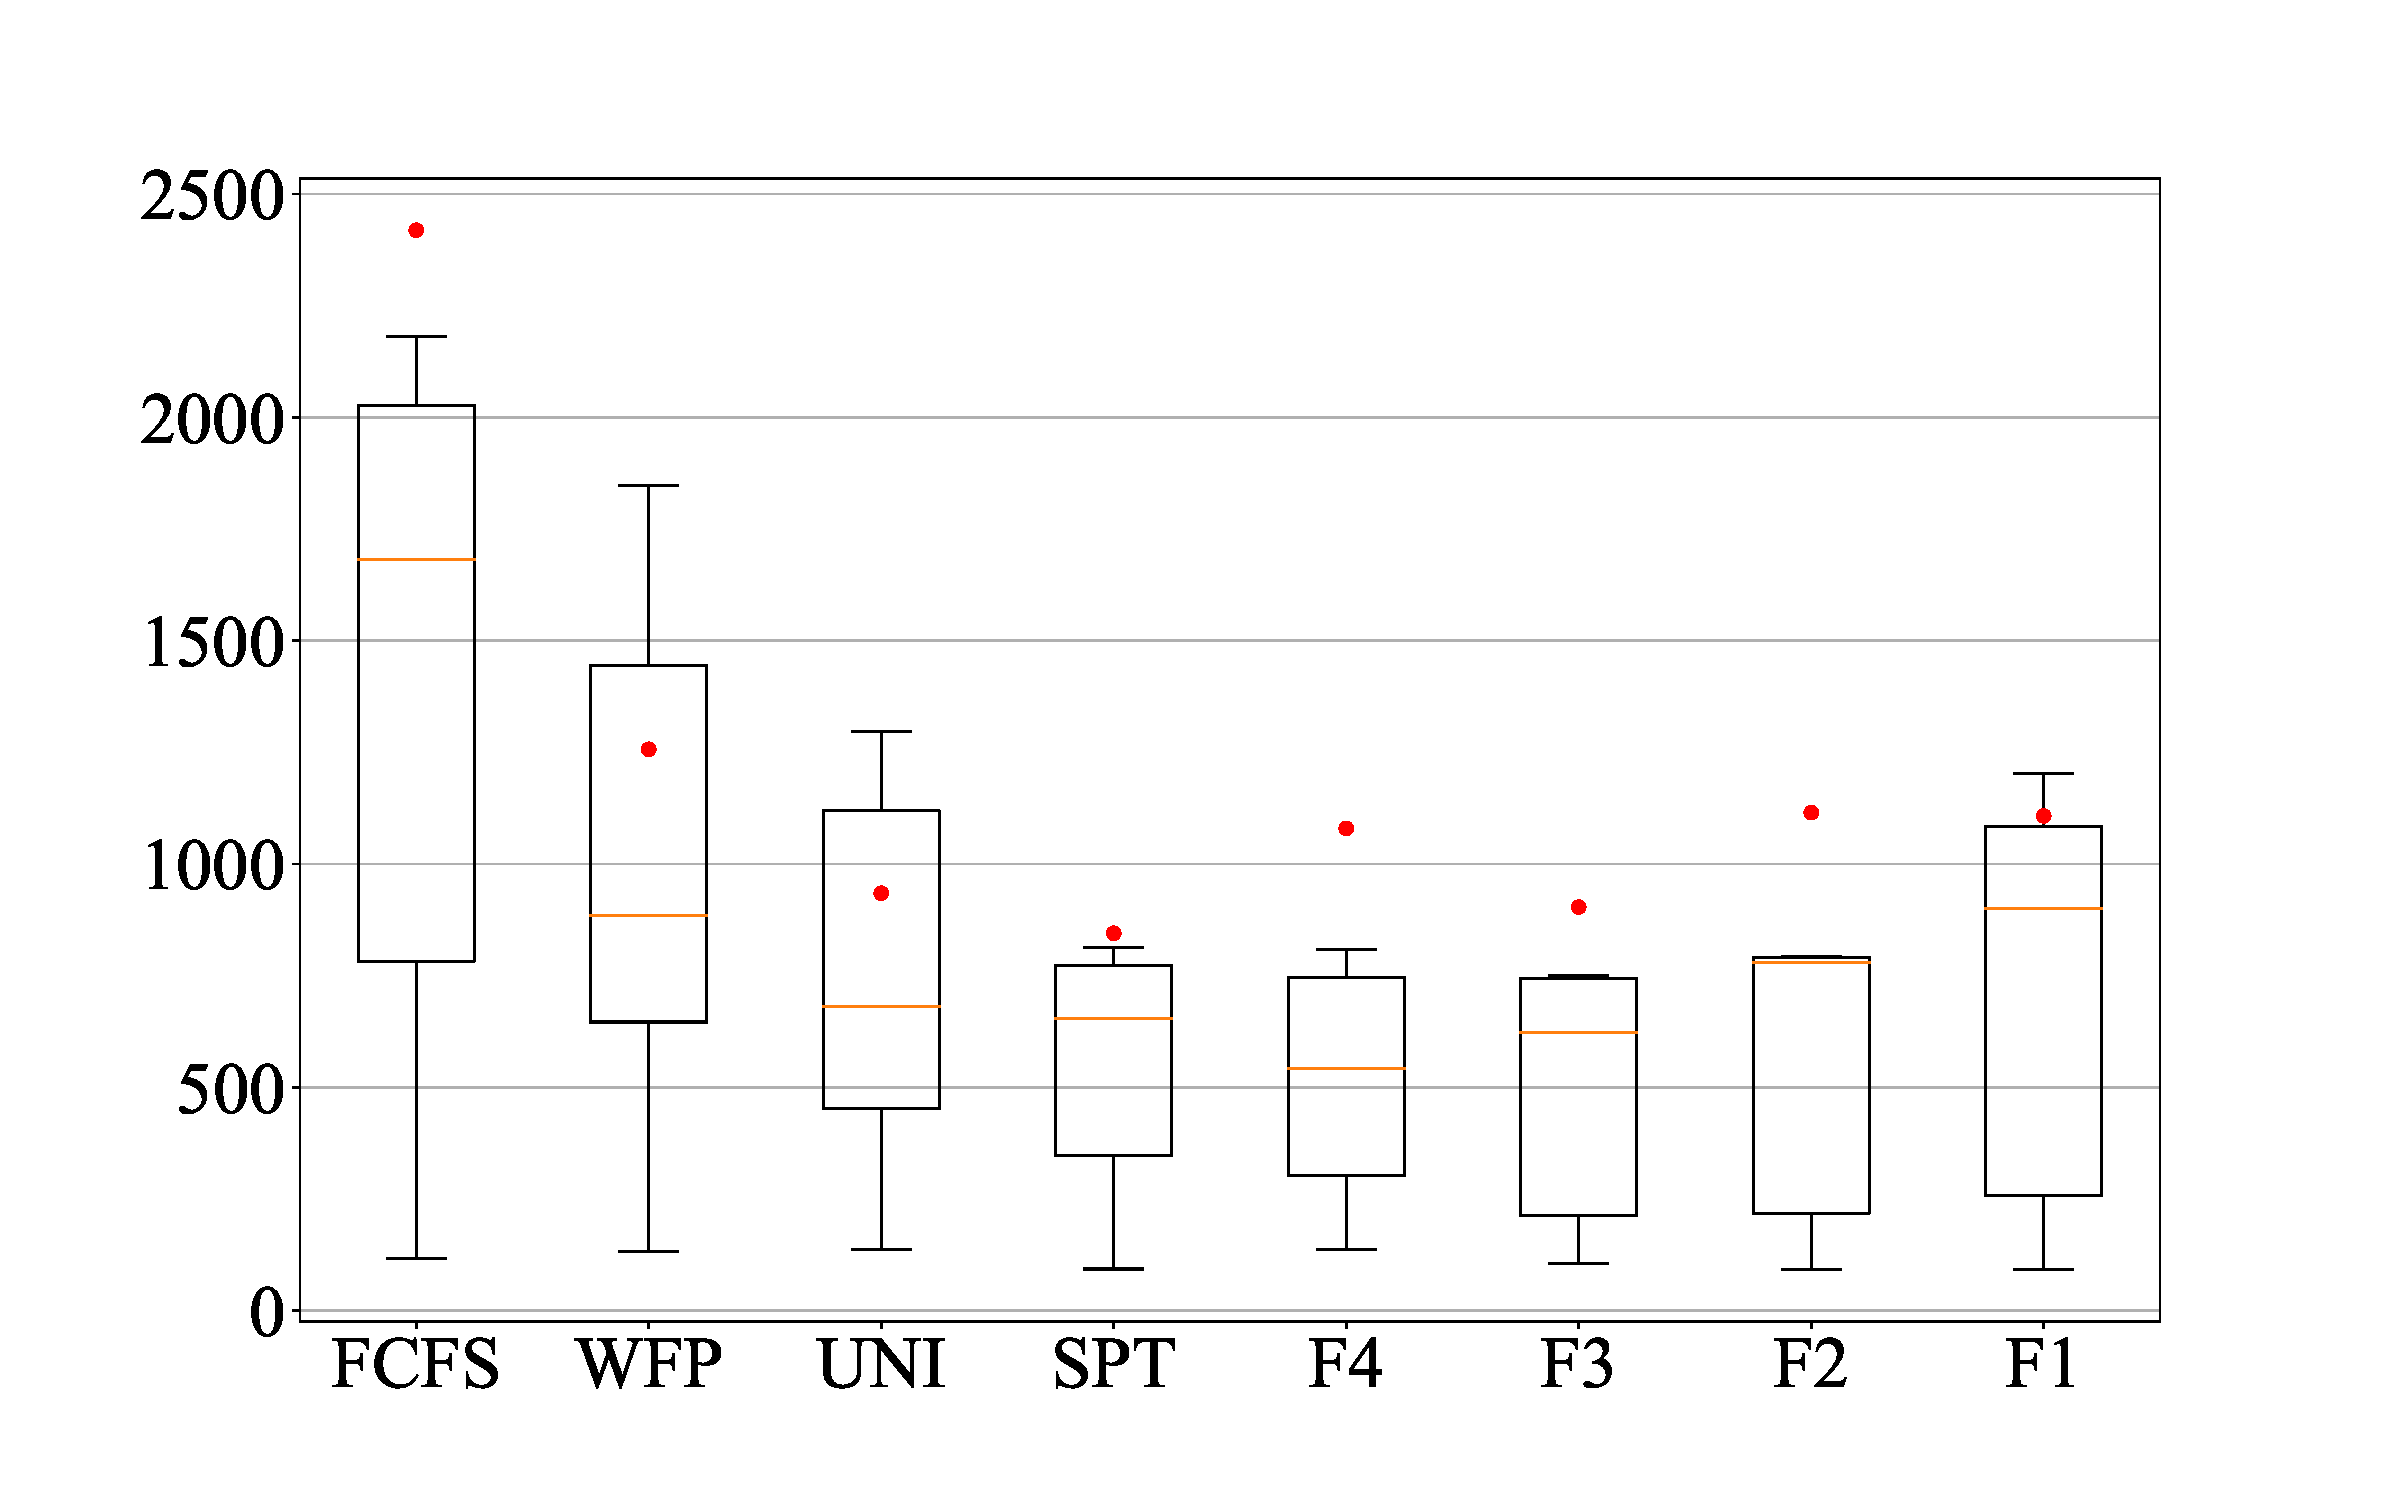
\includegraphics[scale=.20]{figs/Fig7d.pdf}
			%\caption{fig2}
		\end{minipage}
	}%
	
	\centering
	\caption{CEA-Curie workload scheduling performance.} \label{Fig:7}
\end{figure}

Figure \ref{Fig:7} shows the scheduling result of the CEA-Curie-2011-2.1-cln workload, and Tables \ref{tbl3}-\ref{tbl6} are the corresponding median and mean values of $A\!V\!Gblsd$ and $A\!V\!Gwt$ with user-requested time and predicted time, respectively.
\begin{table}[width=.60\linewidth,cols=9,pos=h]
	\caption{Median and mean $A\!V\!Gblsd$ scheduling performance with $t_{req}$ of CEA-Curie workload.}\label{tbl3}
	\begin{tabular*}{\tblwidth}{@{} LLLLLLLLL@{} }
		\toprule
		Indicator & FCFS & WFP & UNI & SPT & F4 & F3 & F2 & F1\\
		\midrule
		Median & 78.8 &	62.2 & 53.3 & 47.9 & 13.7 & 26.7 & 25.9 & 28.8 \\
		Mean & 104.5 & 85.9 & 76.4 & 72.9 & 23.8 & 37.9 & 36.8 & 40.4\\
		\bottomrule
	\end{tabular*}
\end{table}
\begin{table}[width=.60\linewidth,cols=9,pos=h]
	\caption{Median and mean $A\!V\!Gblsd$ scheduling performance with $t_{pred}$ of CEA-Curie workload.}\label{tbl4}
	\begin{tabular*}{\tblwidth}{@{} LLLLLLLLL@{} }
		\toprule
		Indicator & FCFS & WFP & UNI & SPT & F4 & F3 & F2 & F1\\
		\midrule
		Median & 32.5 & 15.4 & 11.8 & 10.7 & \textbf{9.7} & 10.9 & 12.1 & 16.2 \\
		Mean & 71.6 & 30.4 & \textbf{17.6} & 19.1 & 35.5 & 26.6 & 34.1 & 31.5\\
		\bottomrule
	\end{tabular*}
\end{table}

For the $A\!V\!Gblsd$ of CEA-Curie-2011-2.1-cln, shown as Table \ref{tbl3} and \ref{tbl4}, except for the mean value of F4, all other scheduling performance is improved by OKCM according to Median and Mean indicators. For the median value, F4 scheduling obtains the optimal performance. In terms of mean value, UNI has the highest performance. UNI achieves the greatest improvement, 4.52 and 4.33 times better than user-requested time for the median and mean, respectively.
\begin{table}[width=.62\linewidth,cols=9,pos=h]
	\caption{Median and mean $A\!V\!Gwt$ scheduling performance with $t_{req}$ of CEA-Curie workload.}\label{tbl5}
	\begin{tabular*}{\tblwidth}{@{} LLLLLLLLL@{} }
		\toprule
		Indicator & FCFS & WFP & UNI & SPT & F4 & F3 & F2 & F1\\
		\midrule
		Median & 2935.3 & 2609.4 & 2067.2 & 1771.0 & 689.7 & 936.9 & 883.6 & 1070.2 \\
		Mean & 3367.4 & 2740.2 & 2386.9 & 2296.9 & 1258.6 & 1329.5 & 1280.2 & 1397.2\\
		\bottomrule
	\end{tabular*}
\end{table}
\begin{table}[width=.62\linewidth,cols=9,pos=h]
	\caption{Median and mean $A\!V\!Gwt$ scheduling performance with $t_{pred}$ of CEA-Curie workload.}\label{tbl6}
	\begin{tabular*}{\tblwidth}{@{} LLLLLLLLL@{} }
		\toprule
		Indicator & FCFS & WFP & UNI & SPT & F4 & F3 & F2 & F1\\
		\midrule
		Median & 1681.9 &	883.7 &	679.7 &	652.9 &	\textbf{541.1} &	622.9 &	779.2 &	899.9 \\
		Mean & 2418.9 &	1256.6 & 934.3 & \textbf{844.7} &	1079.3 & 903.2 & 1114.8 & 1107.4\\
		\bottomrule
	\end{tabular*}
\end{table}

For the $A\!V\!Gwt$ of CEA-Curie-2011-2.1-cln, shown as Table \ref{tbl5} and \ref{tbl6}, all scheduling performance is improved by OKCM according to Median and Mean indicators. For the median value, F4 scheduling obtains the optimal performance, and UNI achieves up to 3.04 times improvement. In terms of the mean, SPT has the highest performance, and also achieves a maximum 2.72 times improvement. 
In addition, scheduling with our prediction runtime resulted in reduced differences between the 25\% and 75\% quartiles on both $A\!V\!Gblsd$ and $A\!V\!Gwt$ for the CEA-Curie-2011-2.1-cln workload.
\subsubsection{ANL-Intrepid scheduling performance}
\begin{figure}[htbp]
	\centering	
	\subfigure[$A\!V\!Gblsd$ with user-requested time]{
		\begin{minipage}[t]{0.44\linewidth}
			\centering
			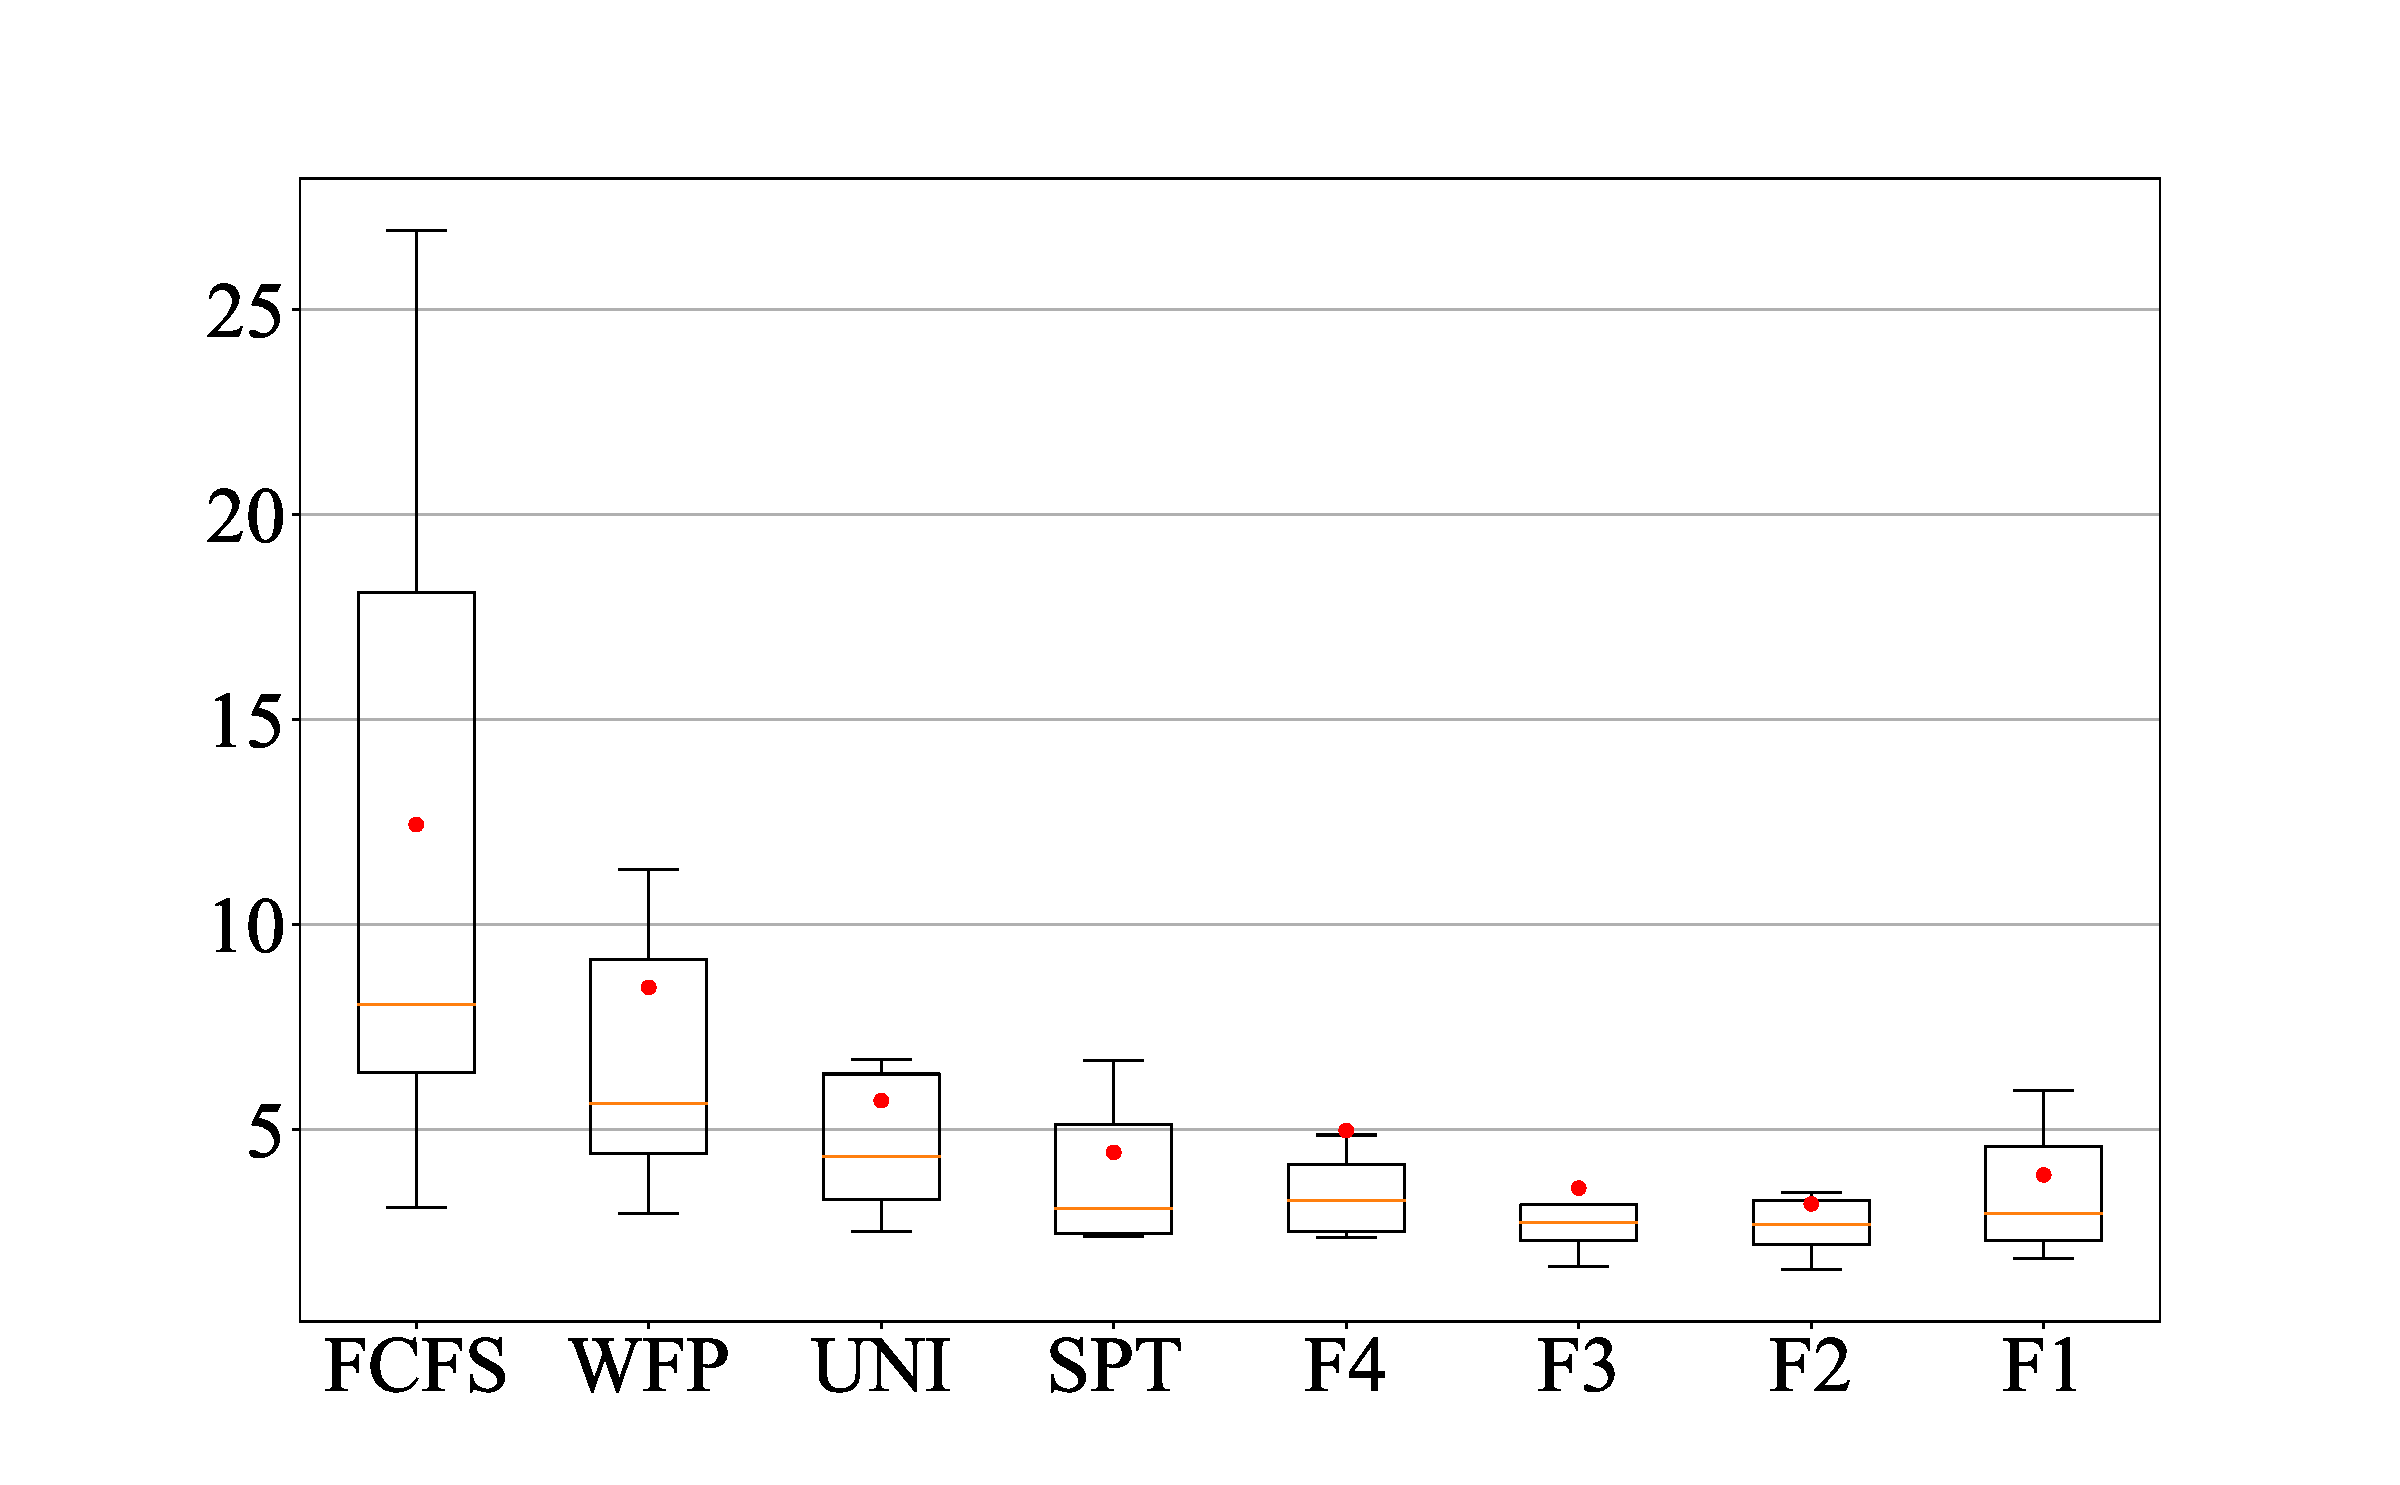
\includegraphics[scale=.20]{figs/Fig8a.pdf}
			%\caption{fig1}
		\end{minipage}%
	}%
	\subfigure[$A\!V\!Gblsd$ with predicted time]{
		\begin{minipage}[t]{0.44\linewidth}
			\centering
			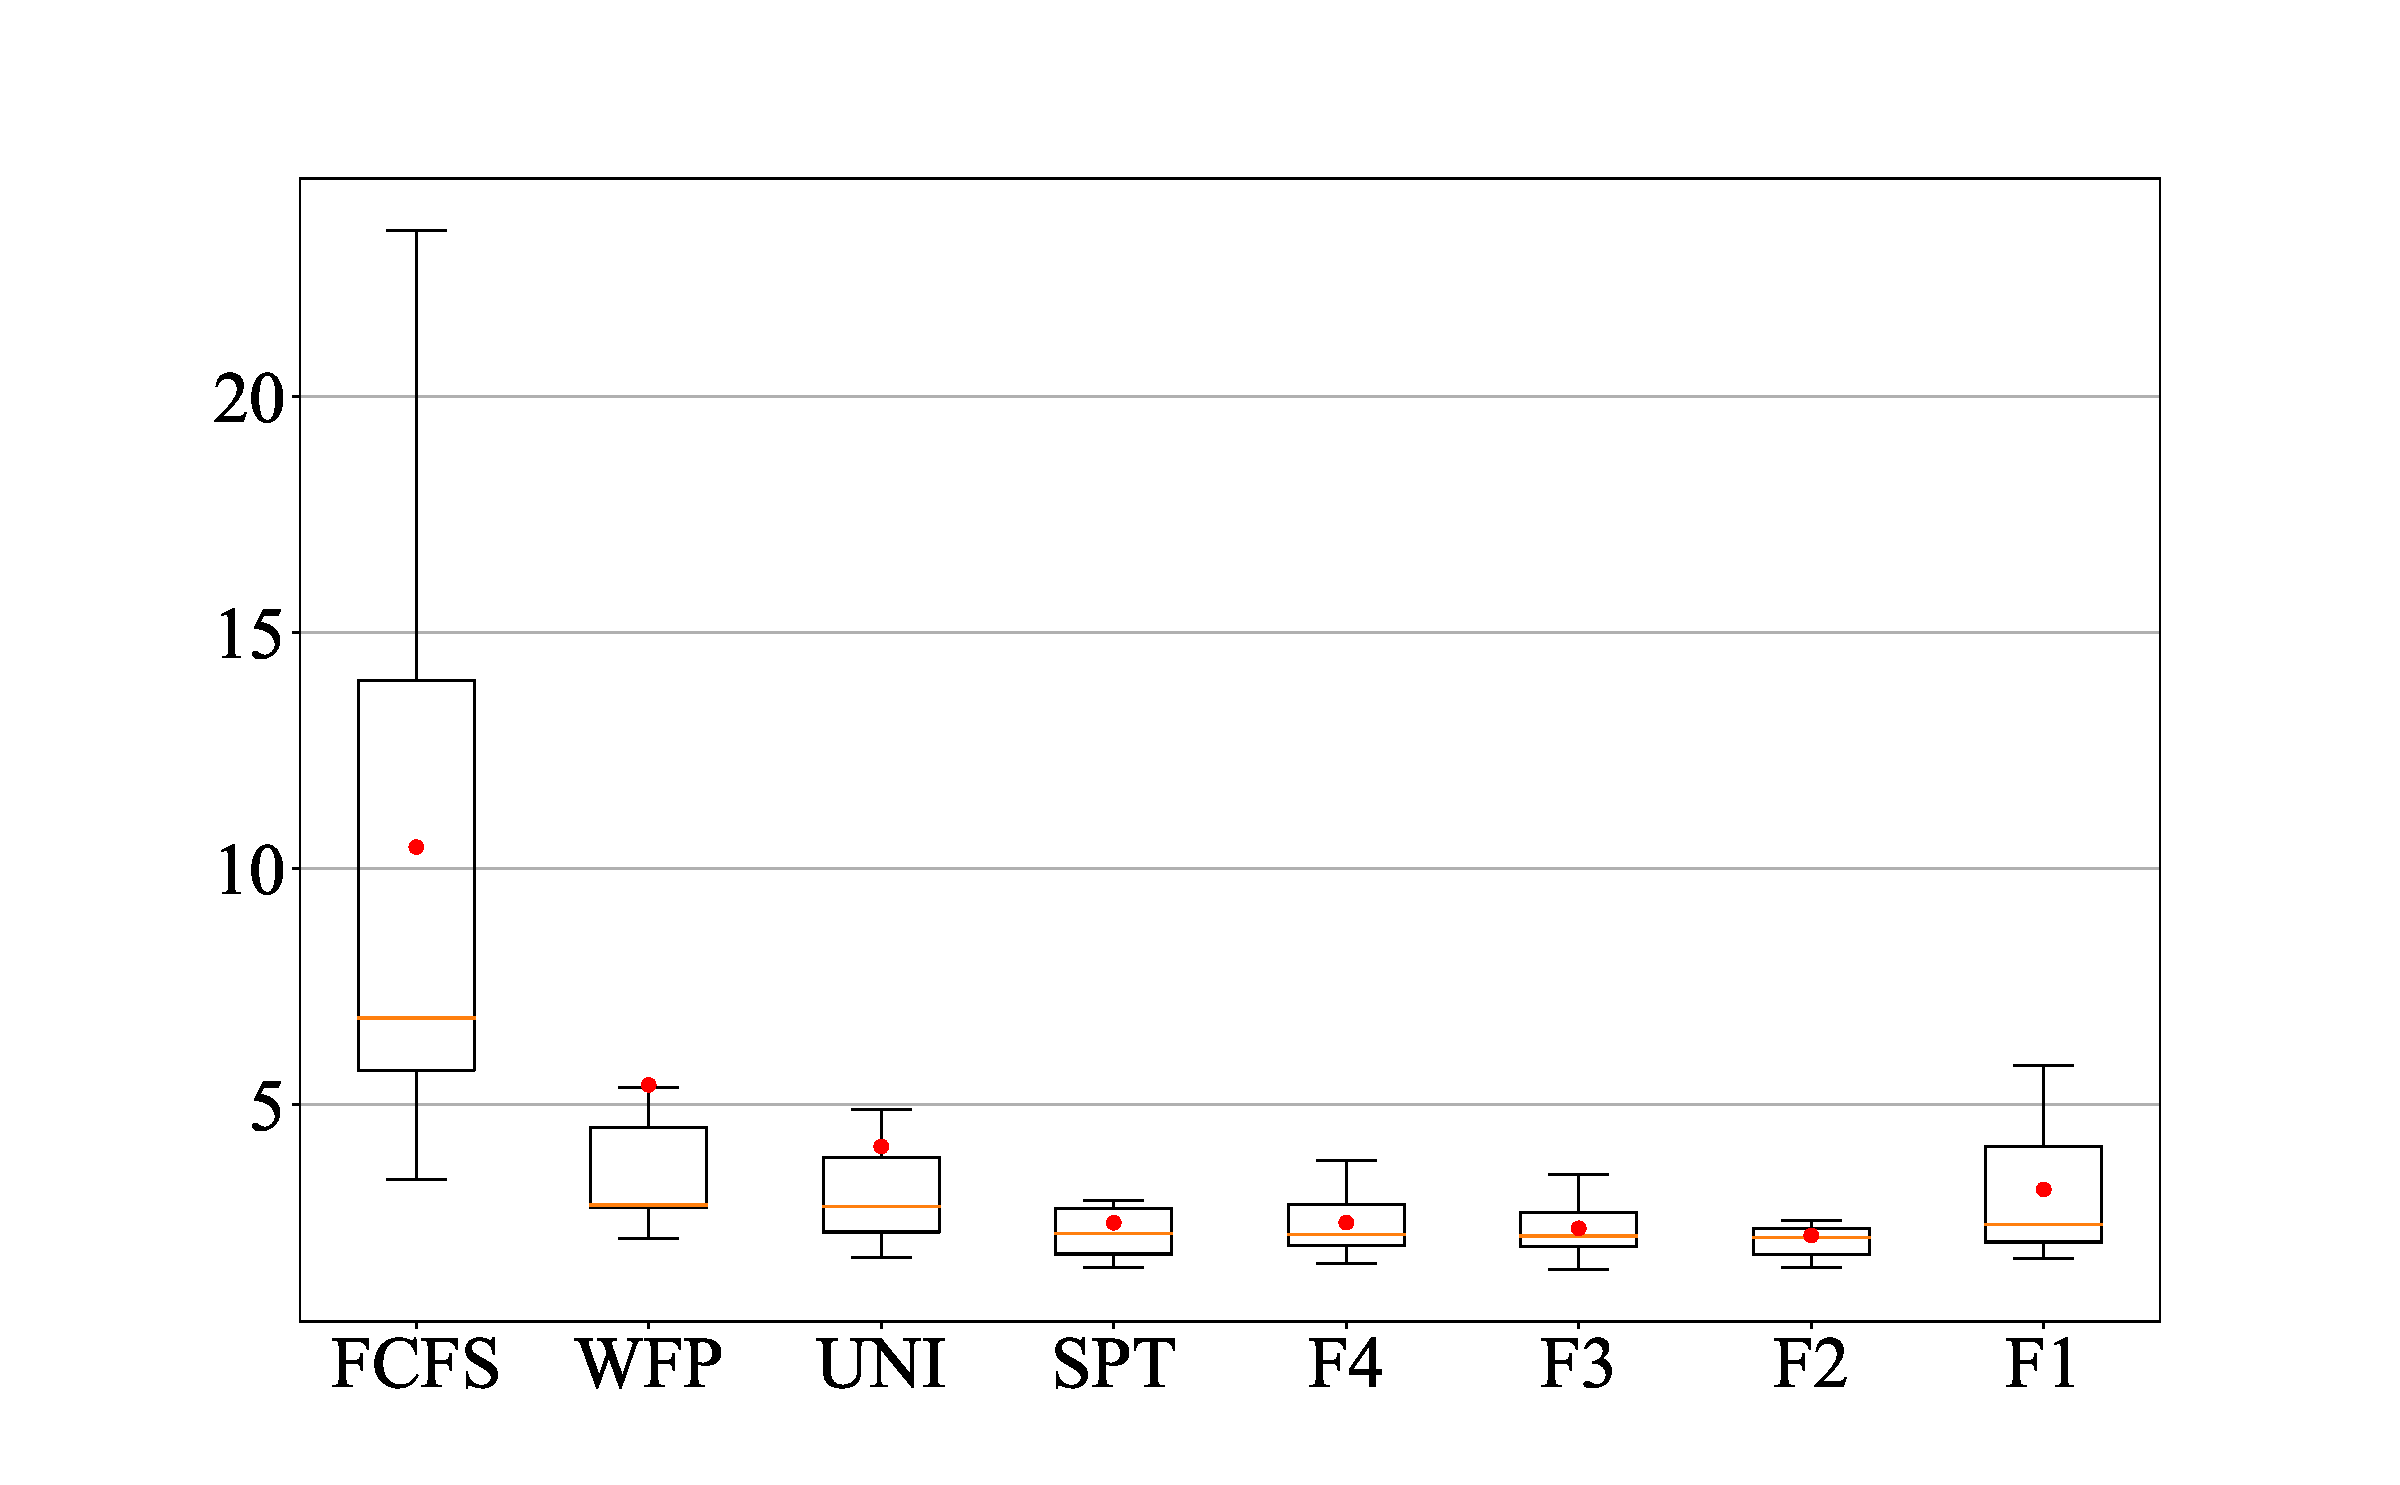
\includegraphics[scale=.20]{figs/Fig8b.pdf}
			%\caption{fig2}
		\end{minipage}%
	}%
	\, %这个回车键很重要 \quad也可以
	\subfigure[$A\!V\!Gwt$ with user-requested time]{
		\begin{minipage}[t]{0.44\linewidth}
			\centering
			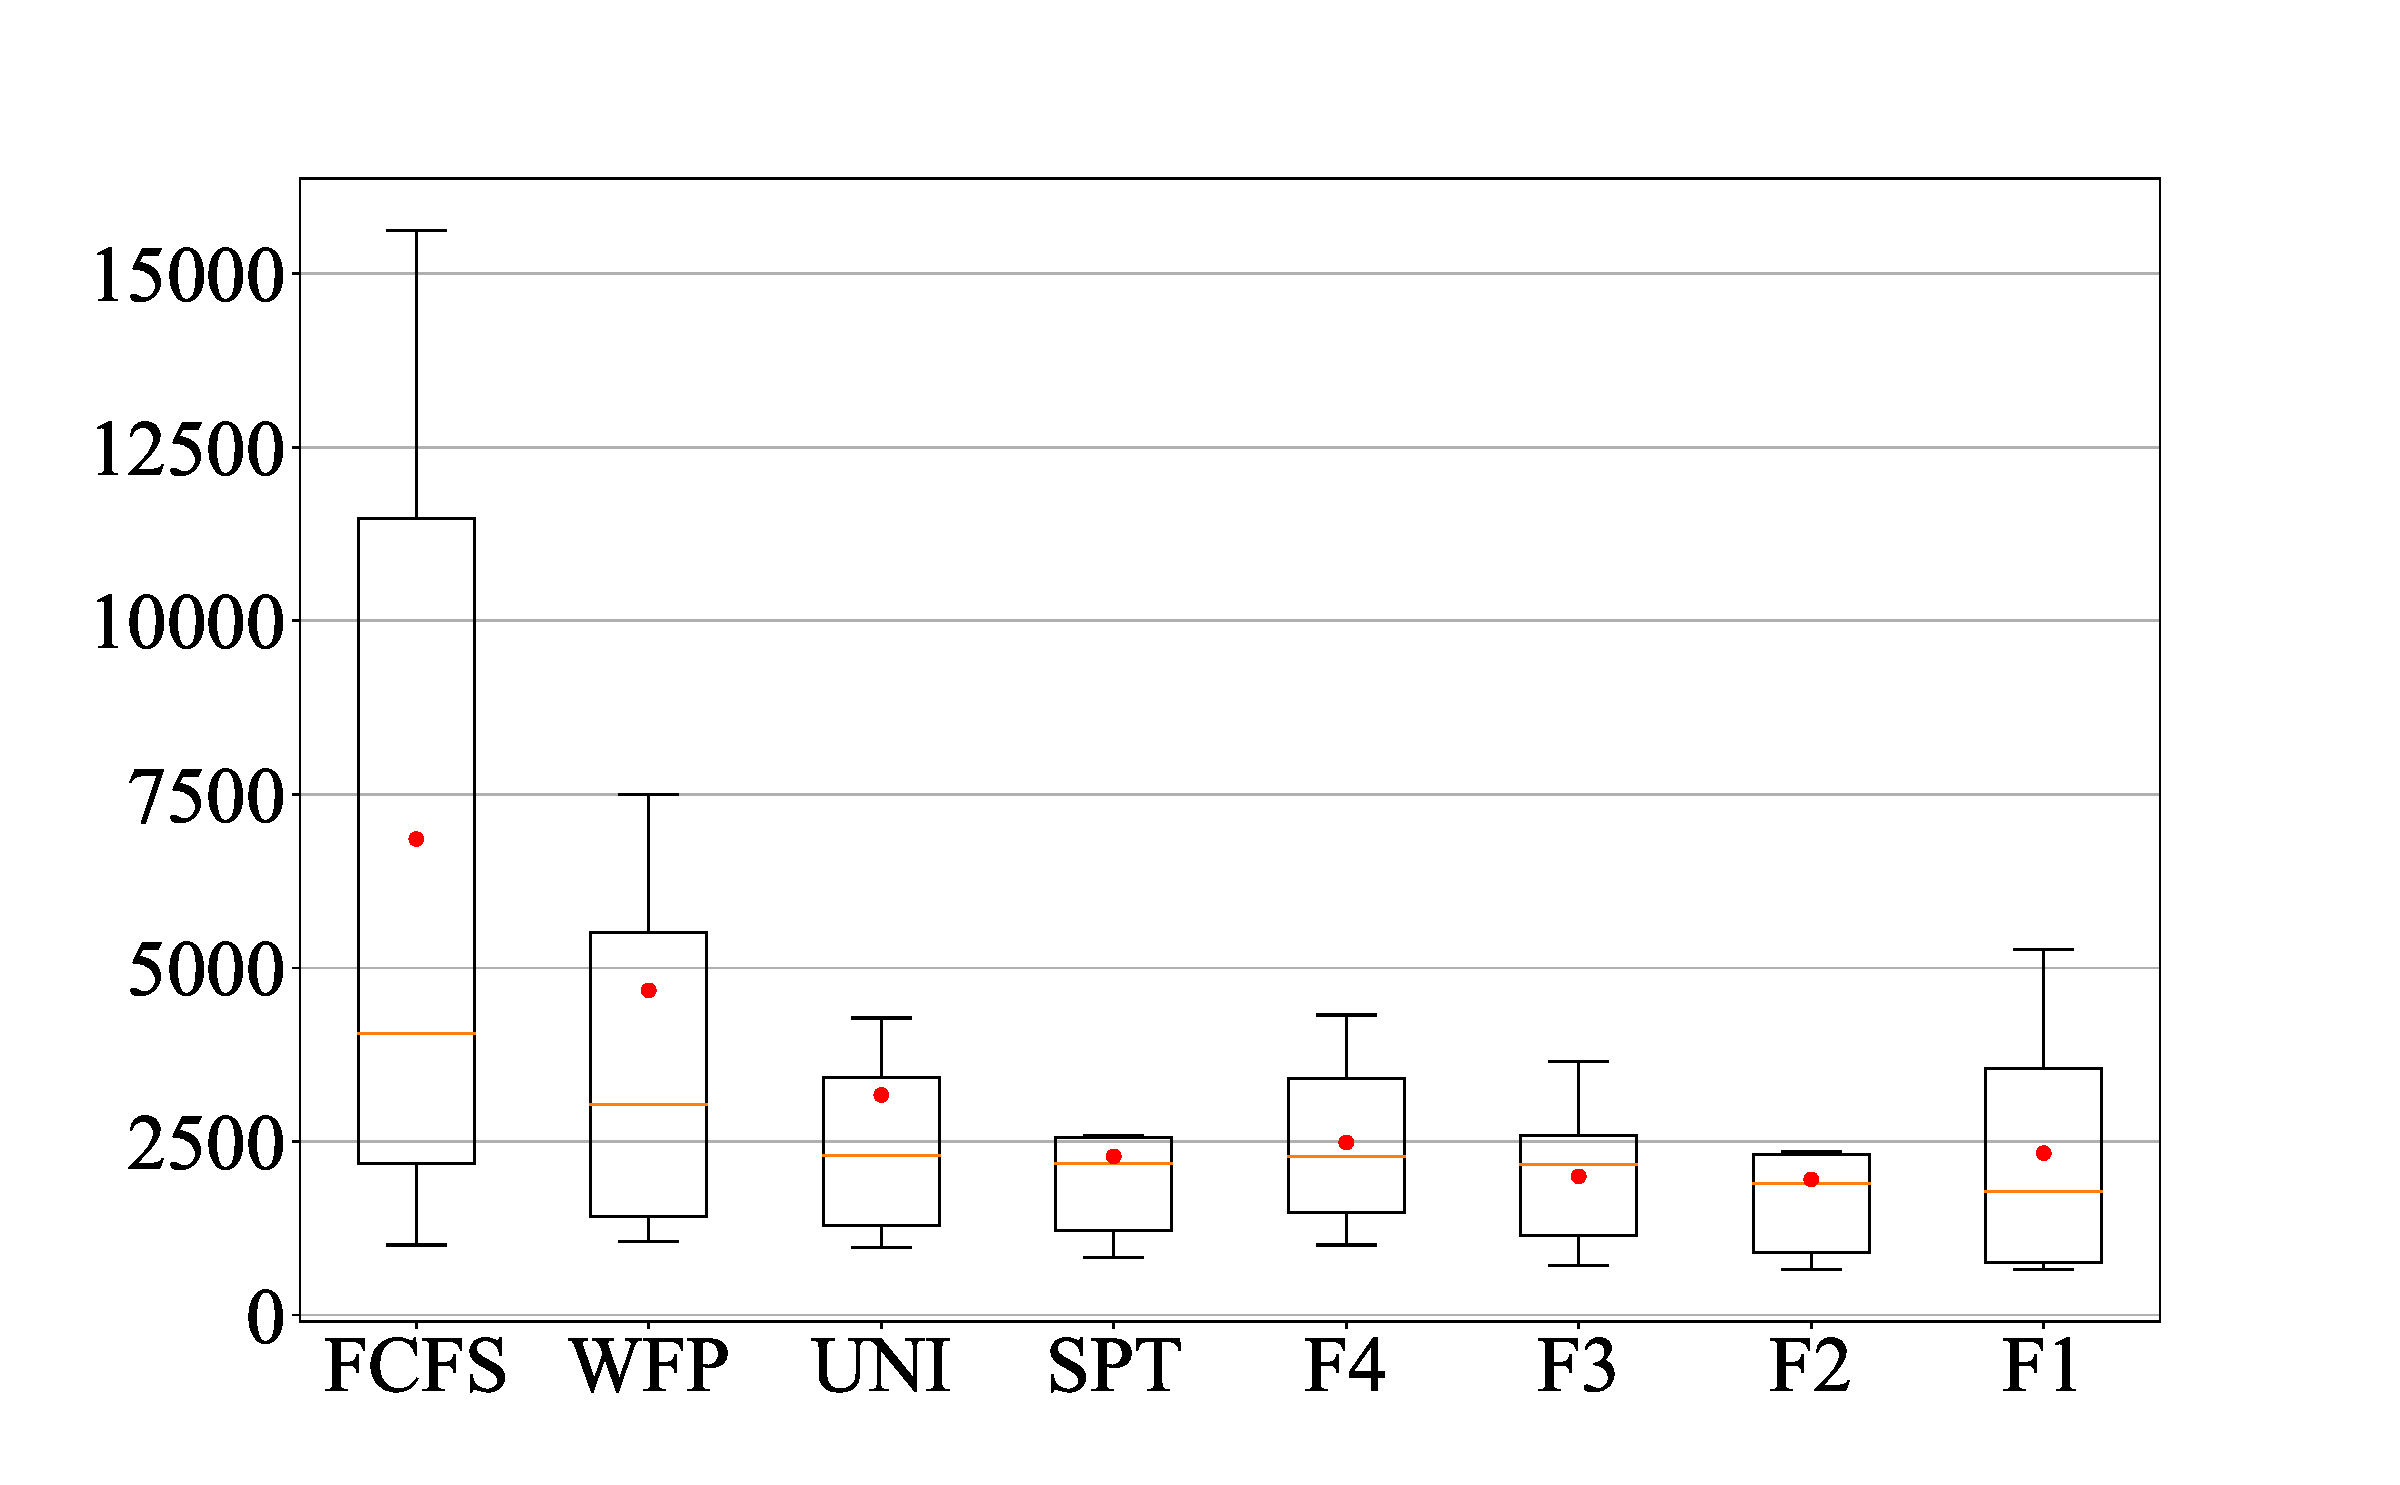
\includegraphics[scale=.20]{figs/Fig8c.pdf}
			%\caption{fig2}
		\end{minipage}
	}%
	\subfigure[$A\!V\!Gwt$ with predicted time]{
		\begin{minipage}[t]{0.44\linewidth}
			\centering
			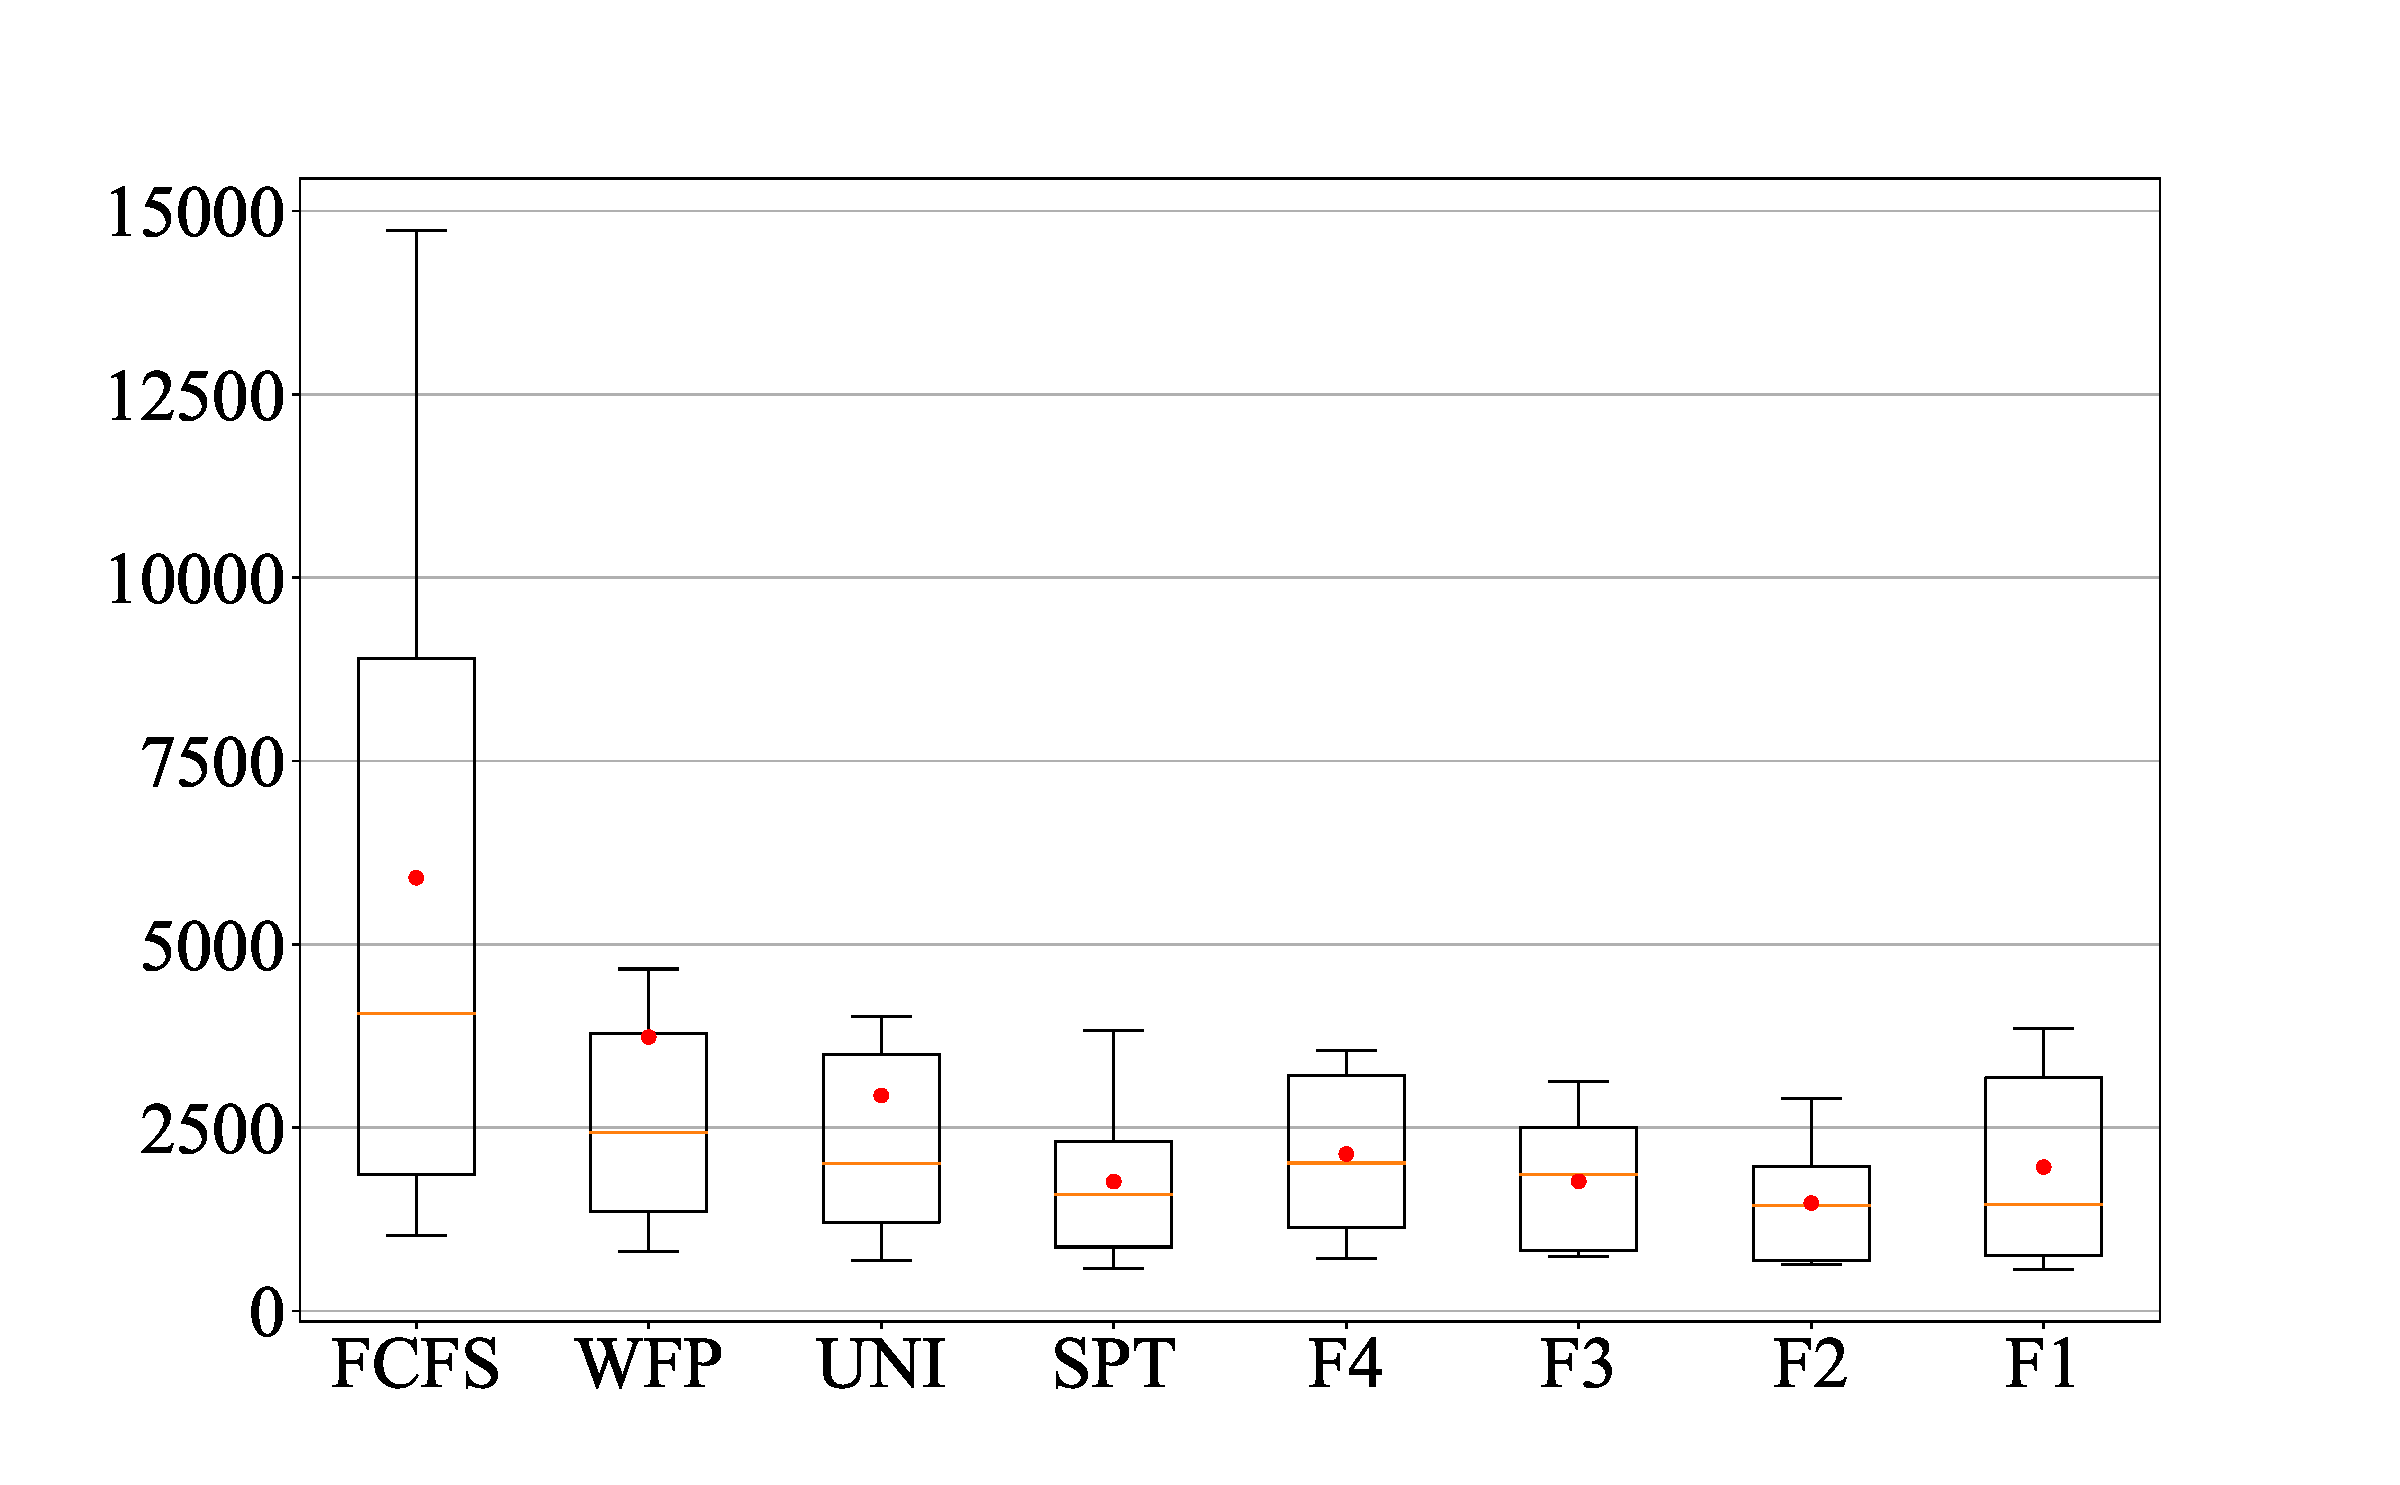
\includegraphics[scale=.20]{figs/Fig8d.pdf}
			%\caption{fig2}
		\end{minipage}
	}%	
	\centering
	\caption{ANL-Intrepid workload scheduling performance.} \label{Fig:8}
\end{figure}
Figure \ref{Fig:8} shows the scheduling result of the ANL-Intrepid-2009-1 workload, and Tables \ref{Fig:7}-\ref{tbl10} are the corresponding median and mean values of $A\!V\!Gblsd$ and $A\!V\!Gwt$ with user-requested time and predicted time, respectively.
\begin{table}[width=.62\linewidth,cols=9,pos=h]
	\caption{Median and mean $A\!V\!Gblsd$ scheduling performance with $t_{req}$ of ANL-Intrepid workload.}\label{tbl7}
	\begin{tabular*}{\tblwidth}{@{} LLLLLLLLL@{} }
		\toprule
		Indicator & FCFS & WFP & UNI & SPT & F4 & F3 & F2 & F1\\
		\midrule
		Median & 8.1 &	5.6 &	4.3 &	3.1 &	3.3 &	2.7 &	2.7 &	3.0 \\
		Mean & 12.4 &	8.5 &	5.7 &	4.4 & 	5.0 &	3.6 &	3.2 &	3.9\\
		\bottomrule
	\end{tabular*}
\end{table}
\begin{table}[width=.62\linewidth,cols=9,pos=h]
	\caption{Median and mean $A\!V\!Gblsd$ scheduling performance with $t_{pred}$ of ANL-Intrepid workload.}\label{tbl8}
	\begin{tabular*}{\tblwidth}{@{} LLLLLLLLL@{} }
		\toprule
		Indicator & FCFS & WFP & UNI & SPT & F4 & F3 & F2 & F1\\
		\midrule
		Median & 6.8 &	2.9 &	2.8 &	2.3 &	2.3 &	2.2 &	\textbf{2.1} &	2.5 \\
		Mean & 10.5 &	5.4 &	4.1 &	2.5 & 2.5 &	2.4 &	\textbf{2.2} &	3.2\\
		\bottomrule
	\end{tabular*}
\end{table}

For the $A\!V\!Gblsd$ of ANL-Intrepid-2009-1 workload, shown as Table \ref{tbl7} and \ref{tbl8}, all scheduling performance is improved by OKCM for Median and Mean indicators. F2 obtains the optimal performance for both indicators. For the median value, WFP achieves up to 1.95 times improvement. In terms of mean, F4 achieves a maximum 1.99 times improvement.
\begin{table}[width=.62\linewidth,cols=9,pos=h]
	\caption{Median and mean $A\!V\!Gwt$ scheduling performance with $t_{req}$ of ANL-Intrepid workload.}\label{tbl9}
	\begin{tabular*}{\tblwidth}{@{} LLLLLLLLL@{} }
		\toprule
		Indicator & FCFS & WFP & UNI & SPT & F4 & F3 & F2 & F1\\
		\midrule
		Median & 4049.0 & 3029.7 &	2304.1 & 2181.2 &	2287.5 & 2169.4 & 1891.7 & 1778.1 \\
		Mean & 6856.1 &	4676.9 & 3169.4 & 2285.8 & 2485.5 & 1997.7 & 1952.9 & 2331.9\\
		\bottomrule
	\end{tabular*}
\end{table}
\begin{table}[width=.62\linewidth,cols=9,pos=h]
	\caption{Median and mean $A\!V\!Gwt$ scheduling performance with $t_{pred}$ of ANL-Intrepid workload.}\label{tbl10}
	\begin{tabular*}{\tblwidth}{@{} LLLLLLLLL@{} }
		\toprule
		Indicator & FCFS & WFP & UNI & SPT & F4 & F3 & F2 & F1\\
		\midrule
		Median & 4061.9 & 2430.6 & 2006.7 & 1595.1 & 2018.8 & 1857.3 & \textbf{1443.3} & 1446.6 \\
		Mean & 5908.3 & 3735.9 & 2939.2 & 1764.8 & 2141.2 & 1768.9 & \textbf{1471.9} & 1962.3 \\
		\bottomrule
	\end{tabular*}
\end{table}

For the $A\!V\!Gwt$ of ANL-Intrepid-2009-1, shown as Table \ref{tbl9} and \ref{tbl10}, except for the median performance of FCFS (decreased by 0.3\%), all other scheduling performance is improved by OKCM for both Median and Mean indicators. F2 obtains the optimal performance for both indicators. SPT achieved the greatest improvement, 1.37 and 1.30 times better than user-requested time for median and mean, respectively.

Scheduling with our prediction runtime resulted in reduced differences between the 25\% and 75\% quartiles on both $A\!V\!Gblsd$ and $A\!V\!Gwt$ for the ANL-Intrepid-2009-1 workload.

\subsubsection{CTC-SP2 scheduling performance}
\begin{figure}[htbp]
	\centering	
	\subfigure[$A\!V\!Gblsd$ with user-requested time]{
		\begin{minipage}[t]{0.44\linewidth}
			\centering
			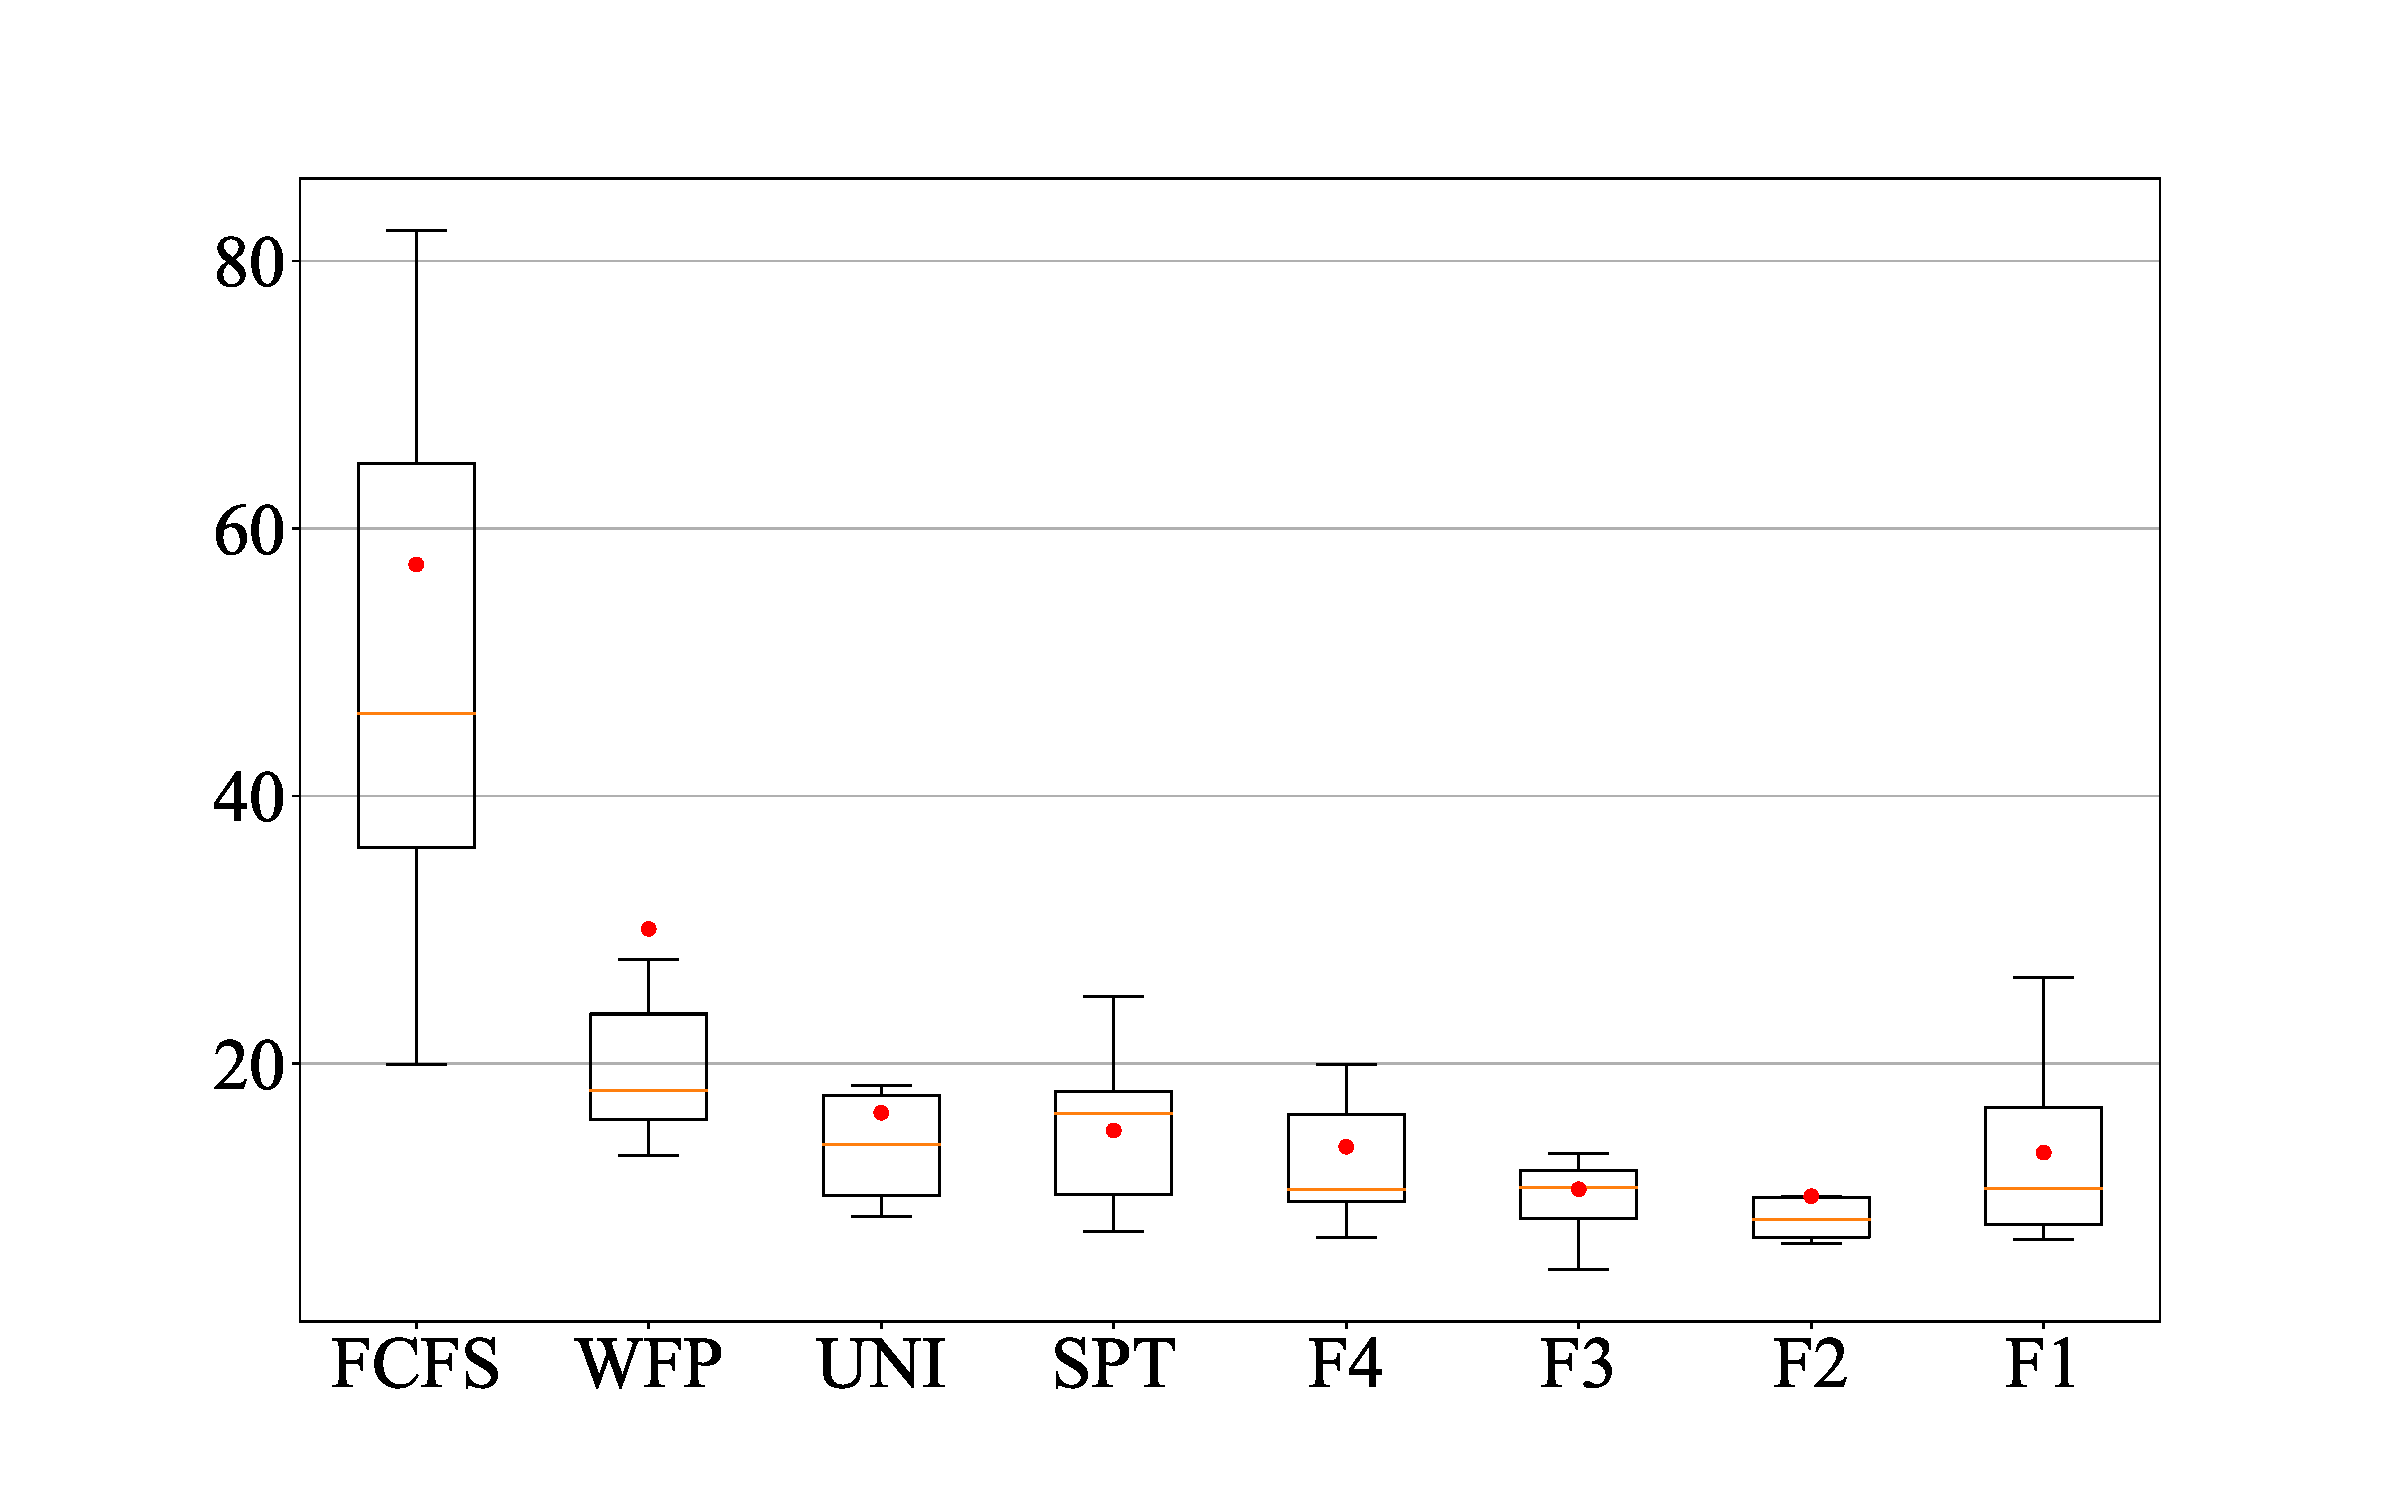
\includegraphics[scale=.20]{figs/Fig9a.pdf}
			%\caption{fig1}
		\end{minipage}%
	}%
	\subfigure[$A\!V\!Gblsd$ with predicted time]{
		\begin{minipage}[t]{0.44\linewidth}
			\centering
			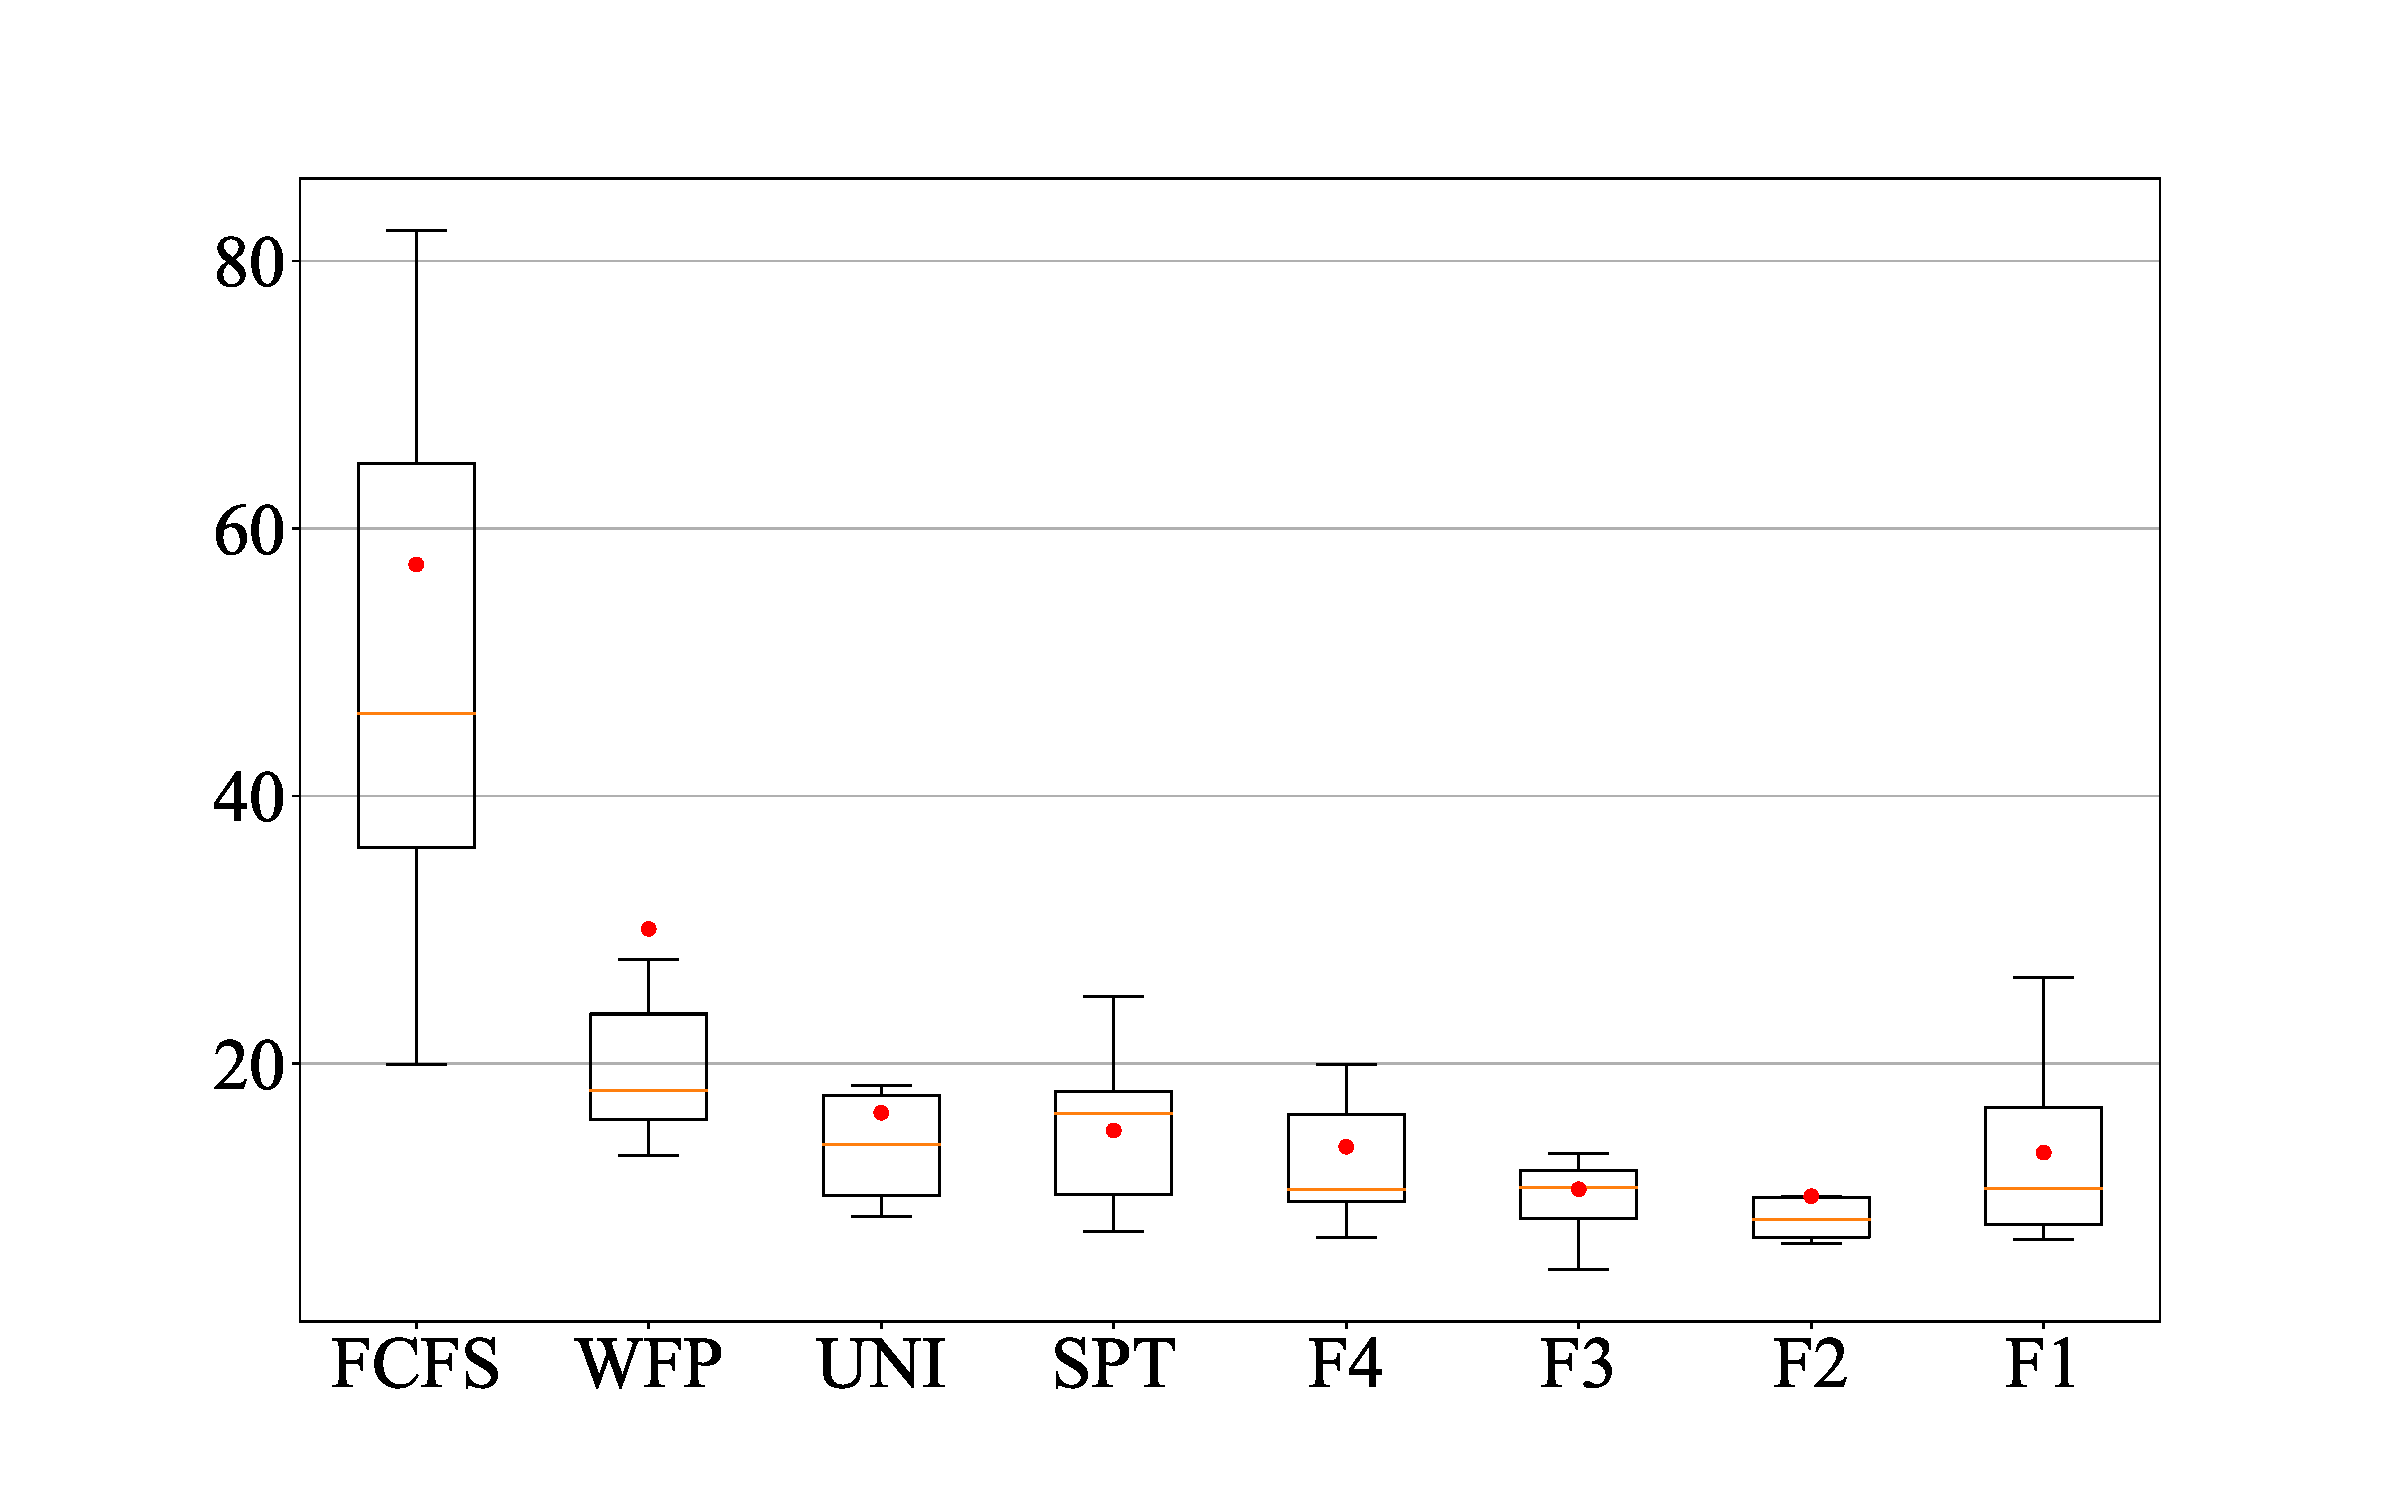
\includegraphics[scale=.20]{figs/Fig9b.pdf}
			%\caption{fig2}
		\end{minipage}%
	}%
	\, %这个回车键很重要 \quad也可以
	\subfigure[$A\!V\!Gwt$ with user-requested time]{
		\begin{minipage}[t]{0.44\linewidth}
			\centering
			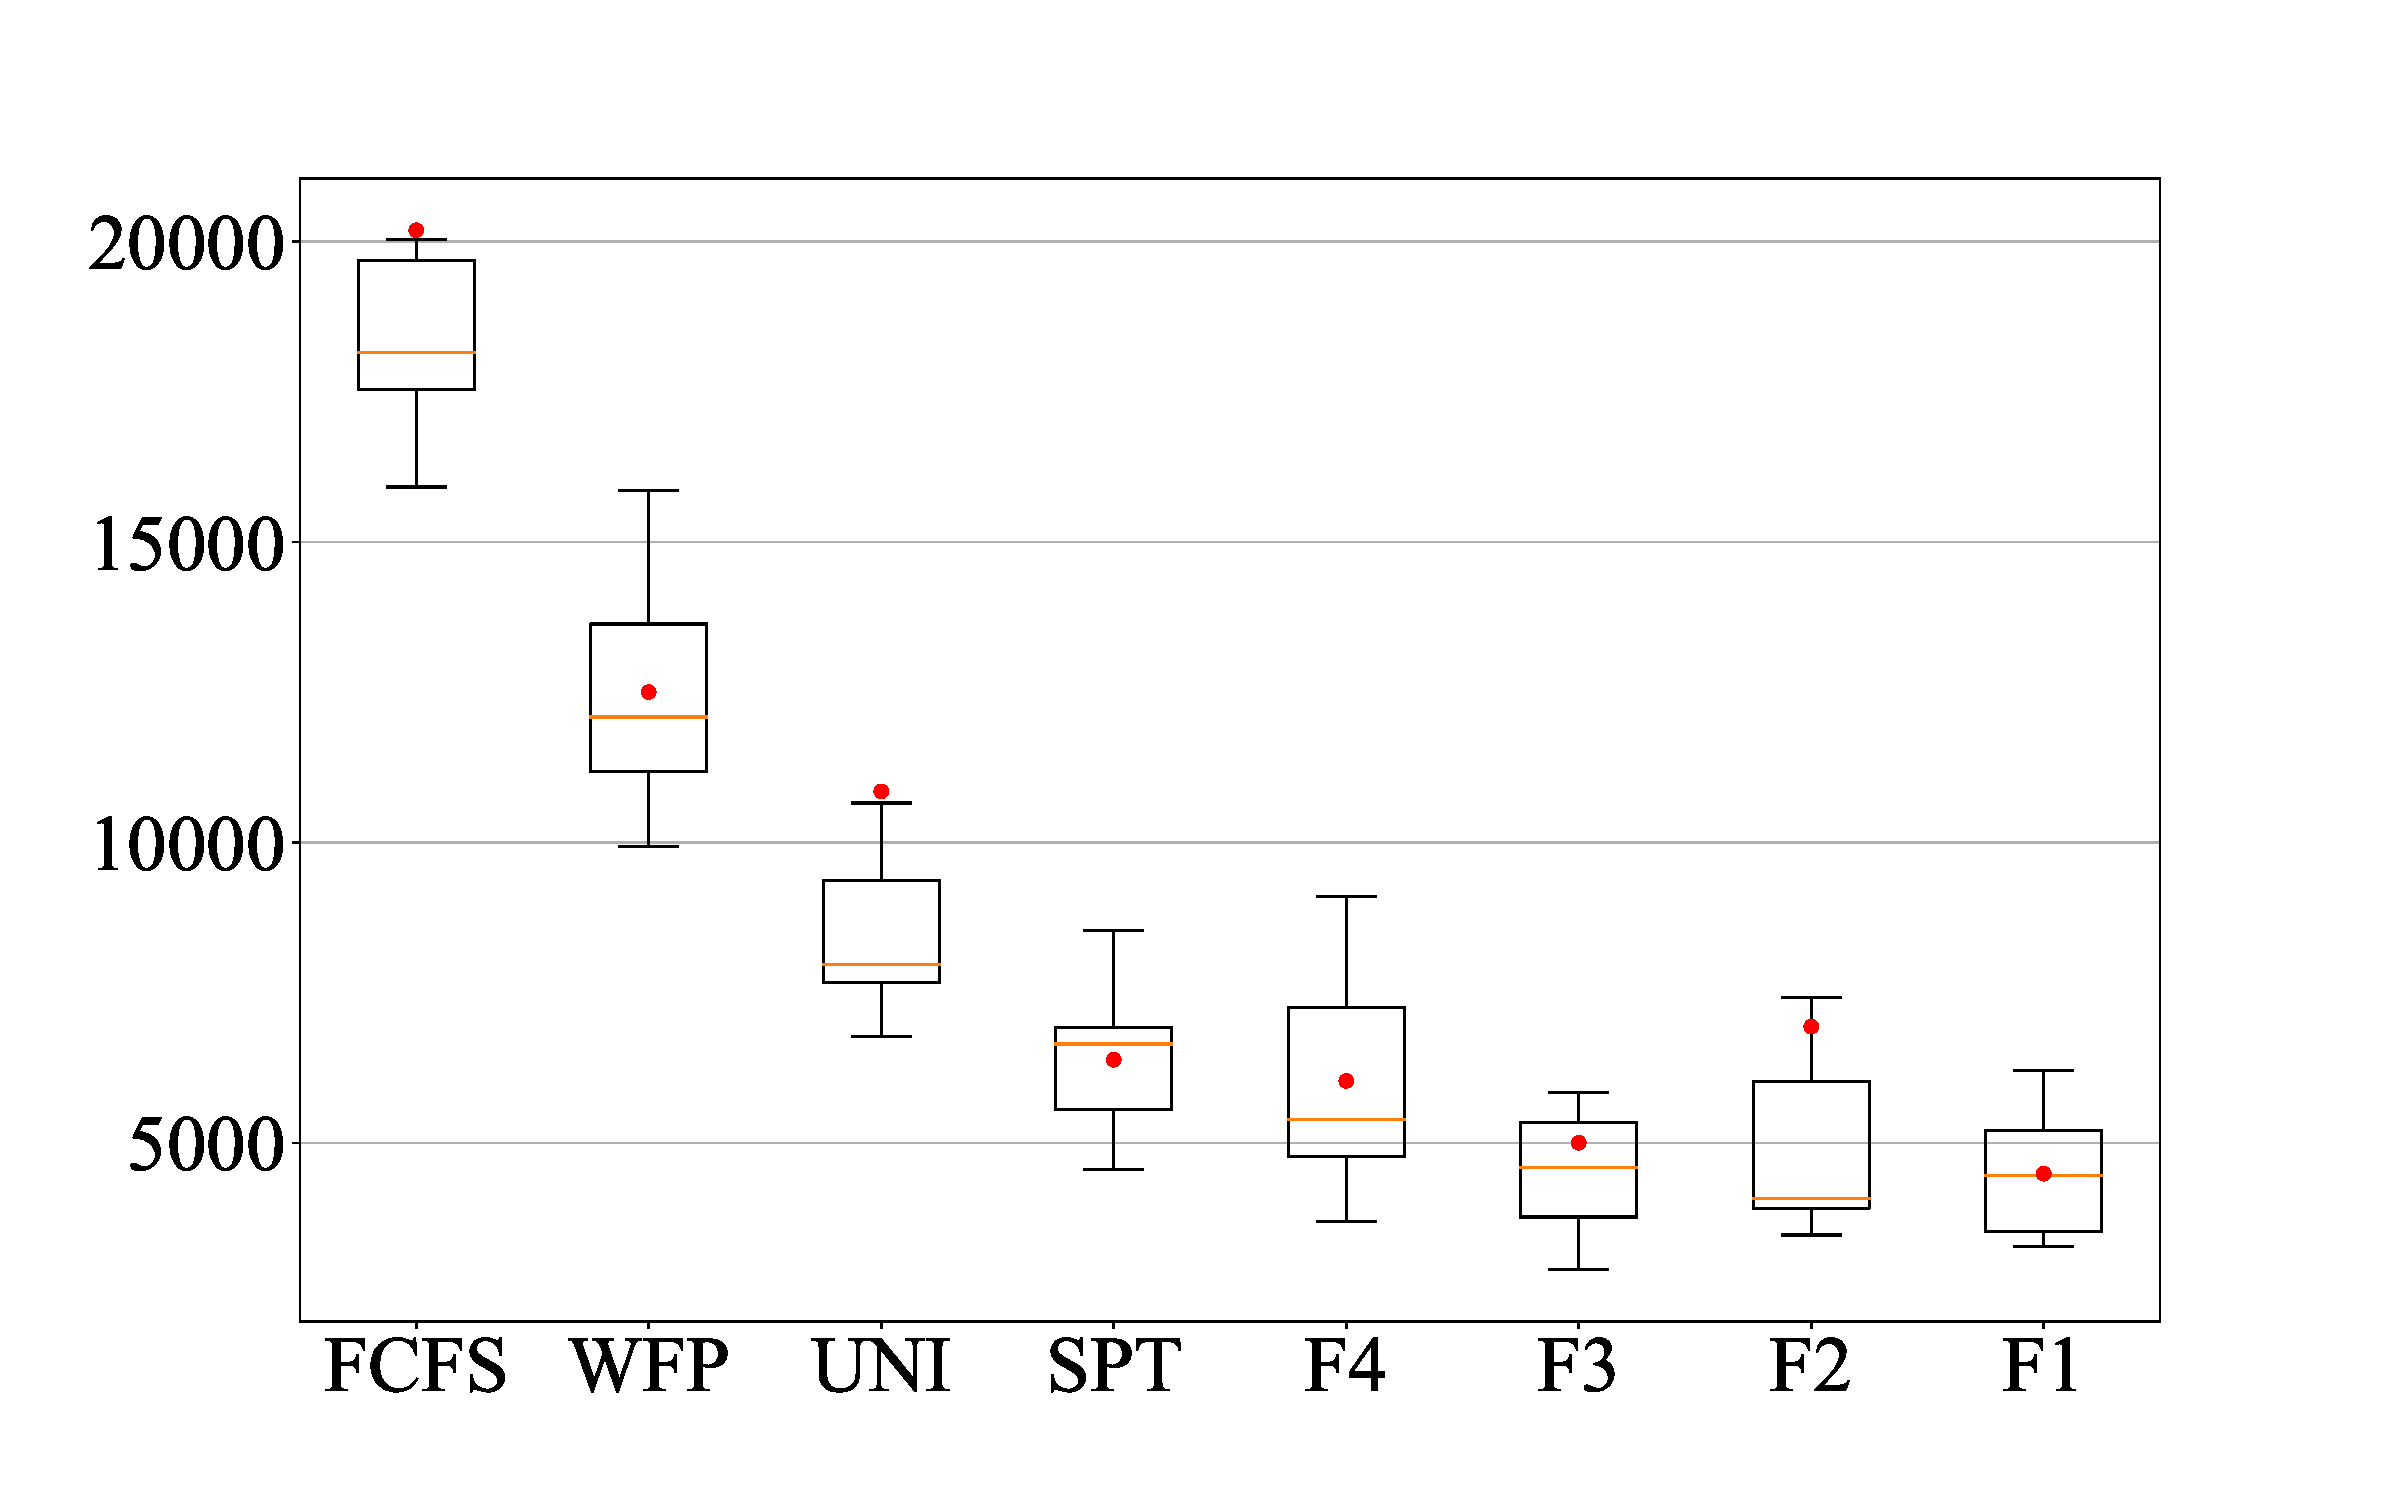
\includegraphics[scale=.20]{figs/Fig9c.pdf}
			%\caption{fig2}
		\end{minipage}
	}%
	\subfigure[$A\!V\!Gwt$ with predicted time]{
		\begin{minipage}[t]{0.44\linewidth}
			\centering
			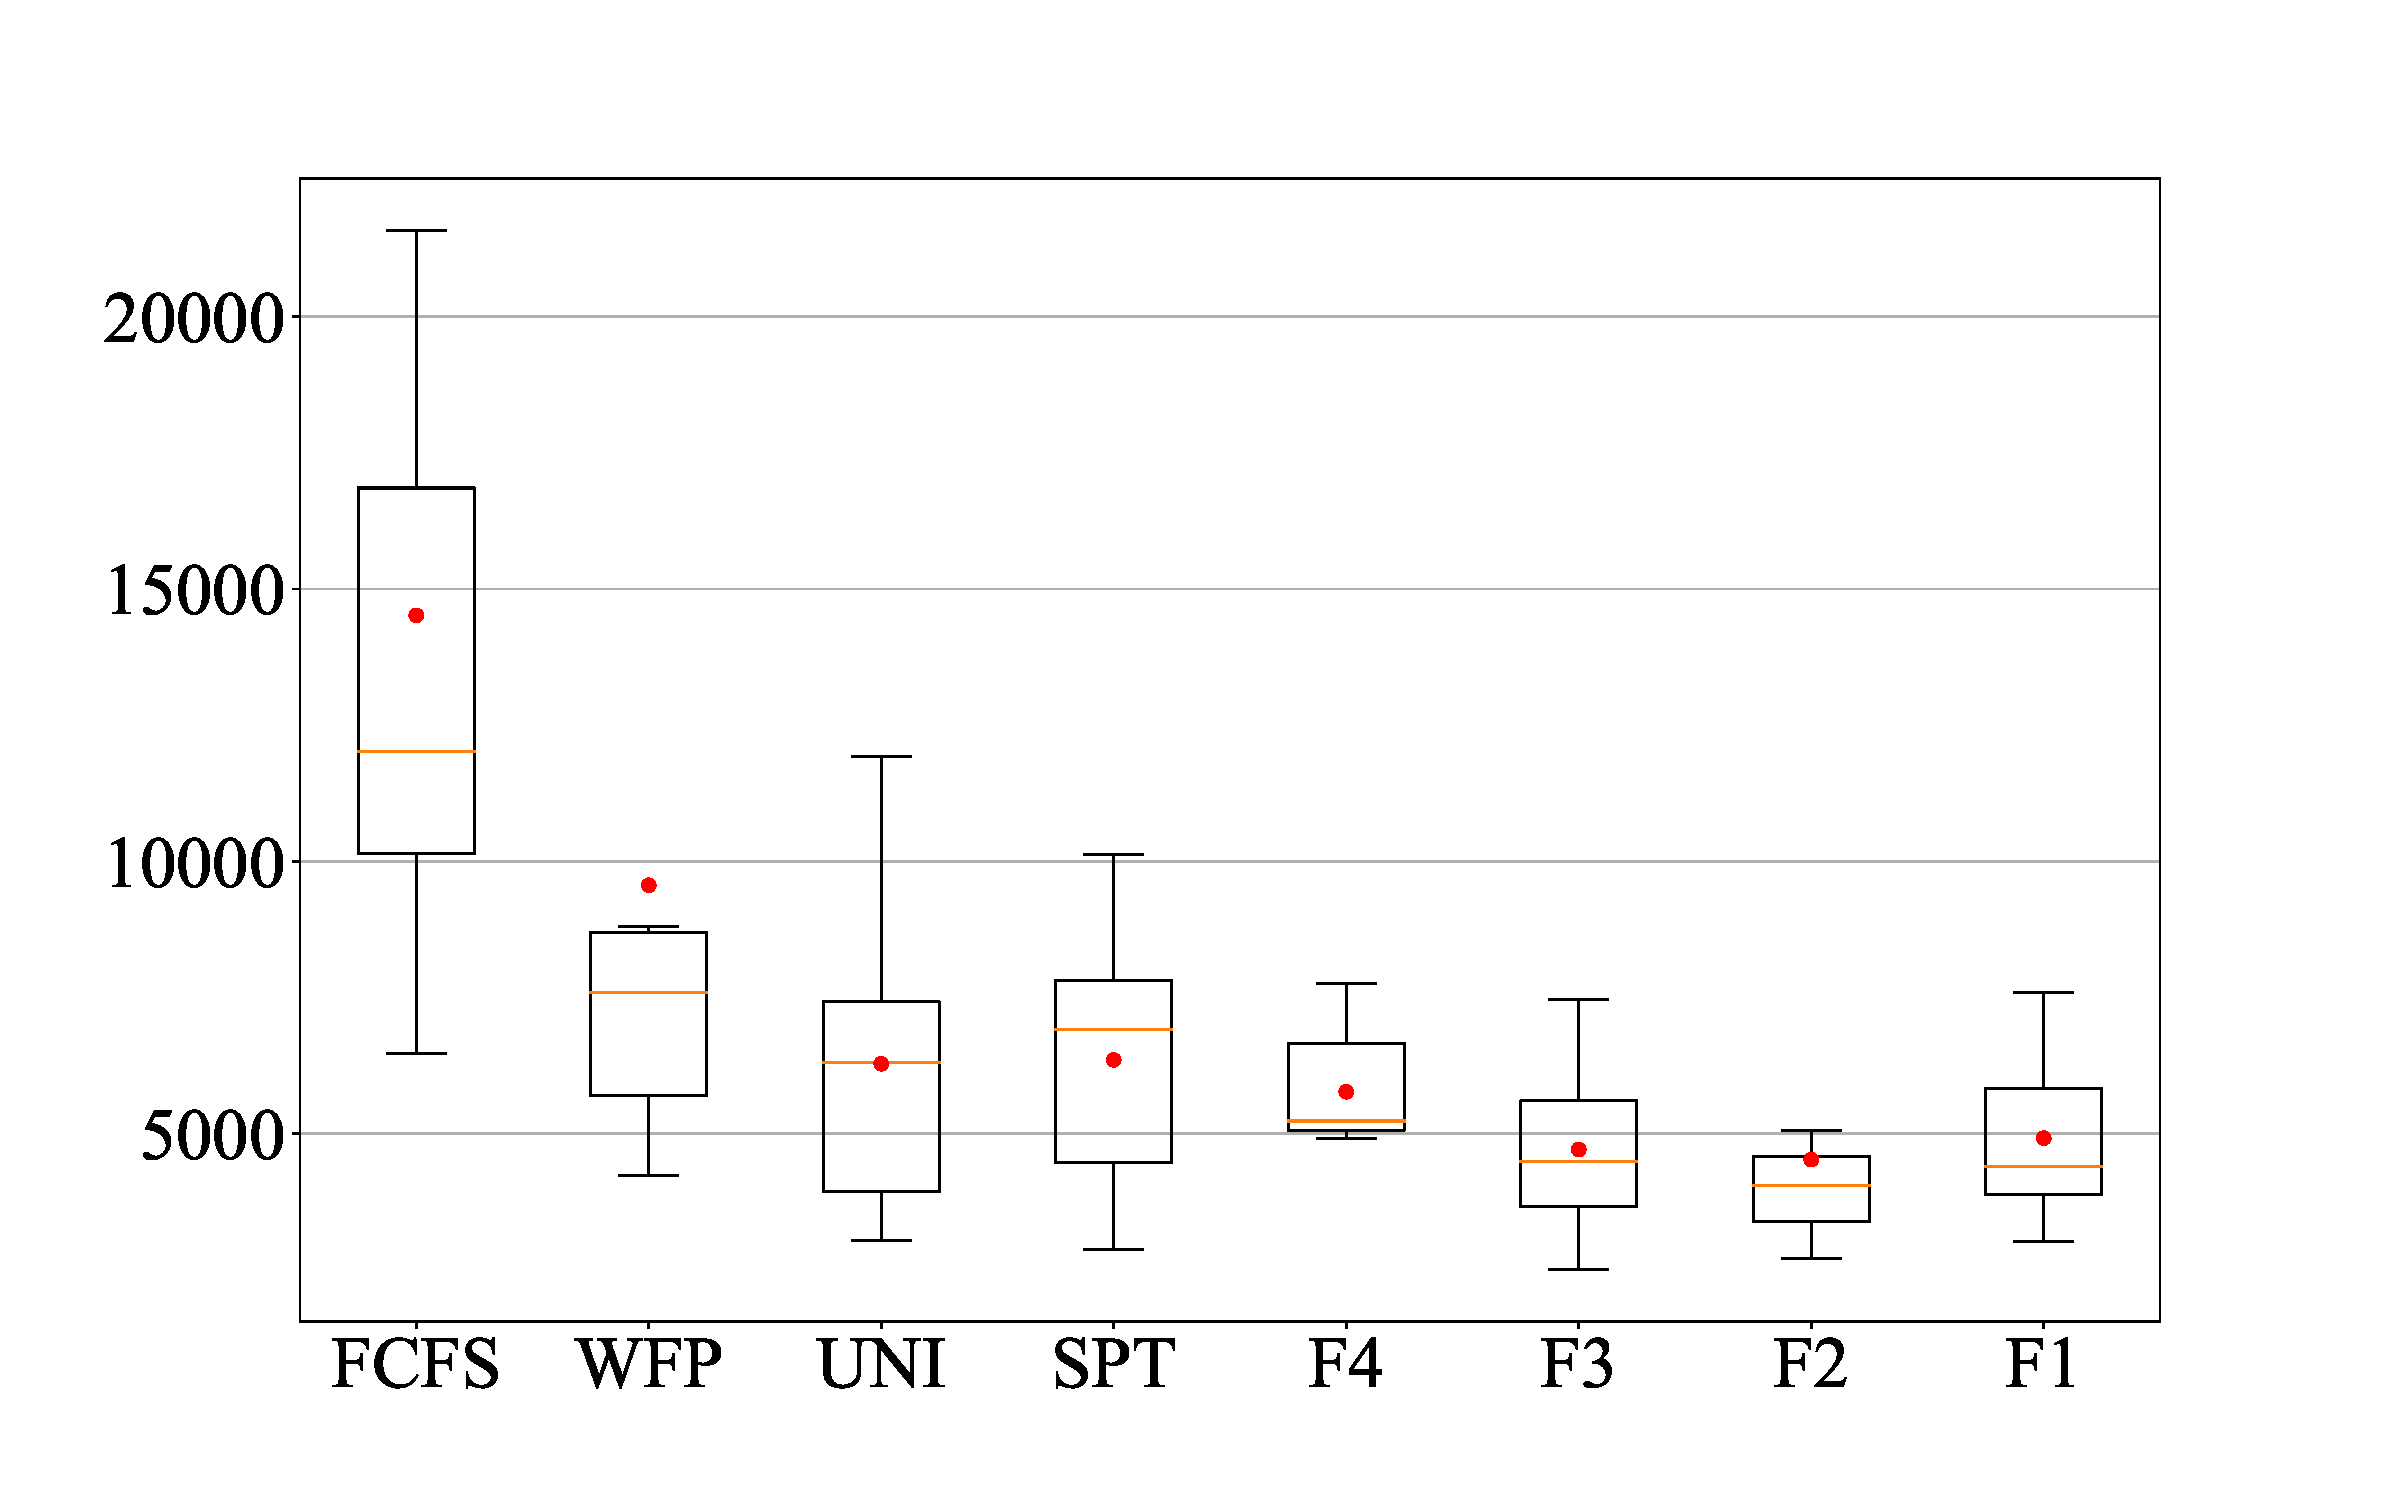
\includegraphics[scale=.20]{figs/Fig9d.pdf}
			%\caption{fig2}
		\end{minipage}
	}%	
	\centering
	\caption{CTC-SP2 workload scheduling performance.} \label{Fig:9}
\end{figure}
Figure \ref{Fig:9} shows the scheduling result of the CTC-SP2-1996-3.1-cln workload, and Tables \ref{tbl11}-\ref{tbl14} are the corresponding median and mean values of $A\!V\!Gblsd$ and $A\!V\!Gwt$ with user-requested time and predicted time, respectively.
\begin{table}[width=.62\linewidth,cols=9,pos=h]
	\caption{Median and mean $A\!V\!Gblsd$ scheduling performance with $t_{req}$ of CTC-SP2 workload.}\label{tbl11}
	\begin{tabular*}{\tblwidth}{@{} LLLLLLLLL@{} }
		\toprule
		Indicator & FCFS & WFP & UNI & SPT & F4 & F3 & F2 & F1\\
		\midrule
		Median &85.8 & 43.8 & 24.3 & 18.2 & 13.0 & 9.3 & 10.4 & 9.1 \\
		Mean & 89.3 & 46.1 & 39.7 & 19.8 & 16.8 & 14.2 & 21.2 & 12.2 \\
		\bottomrule
	\end{tabular*}
\end{table}
\begin{table}[width=.62\linewidth,cols=9,pos=h]
	\caption{Median and mean $A\!V\!Gblsd$ scheduling performance with $t_{pred}$ of CTC-SP2 workload.}\label{tbl12}
	\begin{tabular*}{\tblwidth}{@{} LLLLLLLLL@{} }
		\toprule
		Indicator & FCFS & WFP & UNI & SPT & F4 & F3 & F2 & F1\\
		\midrule
		Median & 46.2 & 18.0 & 13.9 & 16.2 & 10.6 & 10.7 & \textbf{8.3} & 10.7 \\
		Mean & 57.3 & 30.1 & 16.3 & 15.0 & 13.8 & 10.6 & \textbf{10.1} & 13.3 \\
		\bottomrule
	\end{tabular*}
\end{table}

For the $A\!V\!Gblsd$ of CTC-SP2-1996-3.1-cln, shown as Table \ref{tbl11} and \ref{tbl12}, except for the median performance of F3 (decreased by 15.1\%), the median of F1 (decreased by 17.6), and the mean of F1 (decreased by 9.0), all other scheduling performance is improved by OKCM according to both indicators. F2 obtains the optimal performance for both indicators. For the median value, WFP achieves up to 2.43 times improvement. In terms of mean, UNI achieves a maximum 2.44 times improvement.
\begin{table}[width=.62\linewidth,cols=9,pos=h]
	\caption{Median and mean $A\!V\!Gwt$ scheduling performance with $t_{req}$ of CTC SP2 workload.}\label{tbl13}
	\begin{tabular*}{\tblwidth}{@{} LLLLLLLLL@{} }
		\toprule
		Indicator & FCFS & WFP & UNI & SPT & F4 & F3 & F2 & F1\\
		\midrule
		Median & 18155.6 & 12089.5 & 7966.9 & 6646.6 &	5388.4 & 4589.8 & 4070.3 & 4465.1 \\
		Mean & 20192.6 & 12504.5 & 10852.1 & 6385.1 & 6031.6 & 5002.1 & 6935.9 & 4487.9 \\
		\bottomrule
	\end{tabular*}
\end{table}
\begin{table}[width=.62\linewidth,cols=9,pos=h]
	\caption{Median and mean $A\!V\!Gwt$ scheduling performance with $t_{pred}$ of CTC SP2 workload.}\label{tbl14}
	\begin{tabular*}{\tblwidth}{@{} LLLLLLLLL@{} }
		\toprule
		Indicator & FCFS & WFP & UNI & SPT & F4 & F3 & F2 & F1\\
		\midrule
		Median & 12012.9 & 7600.4 & 6306.8 & 6913.5 & 5233.2 & 4484.9 & \textbf{4043.9} & 4399.4 \\
		Mean & 14515.1 & 9562.1 & 6282.8 & 6355.8 & 5768.8 & 4709.9 & \textbf{4523.9} & 4919.1 \\
		\bottomrule
	\end{tabular*}
\end{table}

For the $A\!V\!Gwt$ of CTC-SP2-1996-3.1-cln, shown as Table \ref{tbl13} and \ref{tbl14}, except for the median performance of SPT (decreased by 4.0\%) and the mean of F1 (decreased by 9.6\%), all other scheduling performance is improved by OKCM according to both indicators. F2 obtains the optimal performance for both indicators. For the median value, SPT achieves up to 1.59 times improvement. In terms of mean, UNI achieves a maximum 1.73 times improvement.

Scheduling with our prediction runtime resulted in reduced differences between the 25\% and 75\% quartiles in both $A\!V\!Gblsd$ and $A\!V\!Gwt$ for the CTC-SP2-1996-3.1-cln workload.

\subsubsection{SDSC-SP2 scheduling performance}
\begin{figure}[htbp]
	\centering	
	\subfigure[$A\!V\!Gblsd$ with user-requested time]{
		\begin{minipage}[t]{0.44\linewidth}
			\centering
			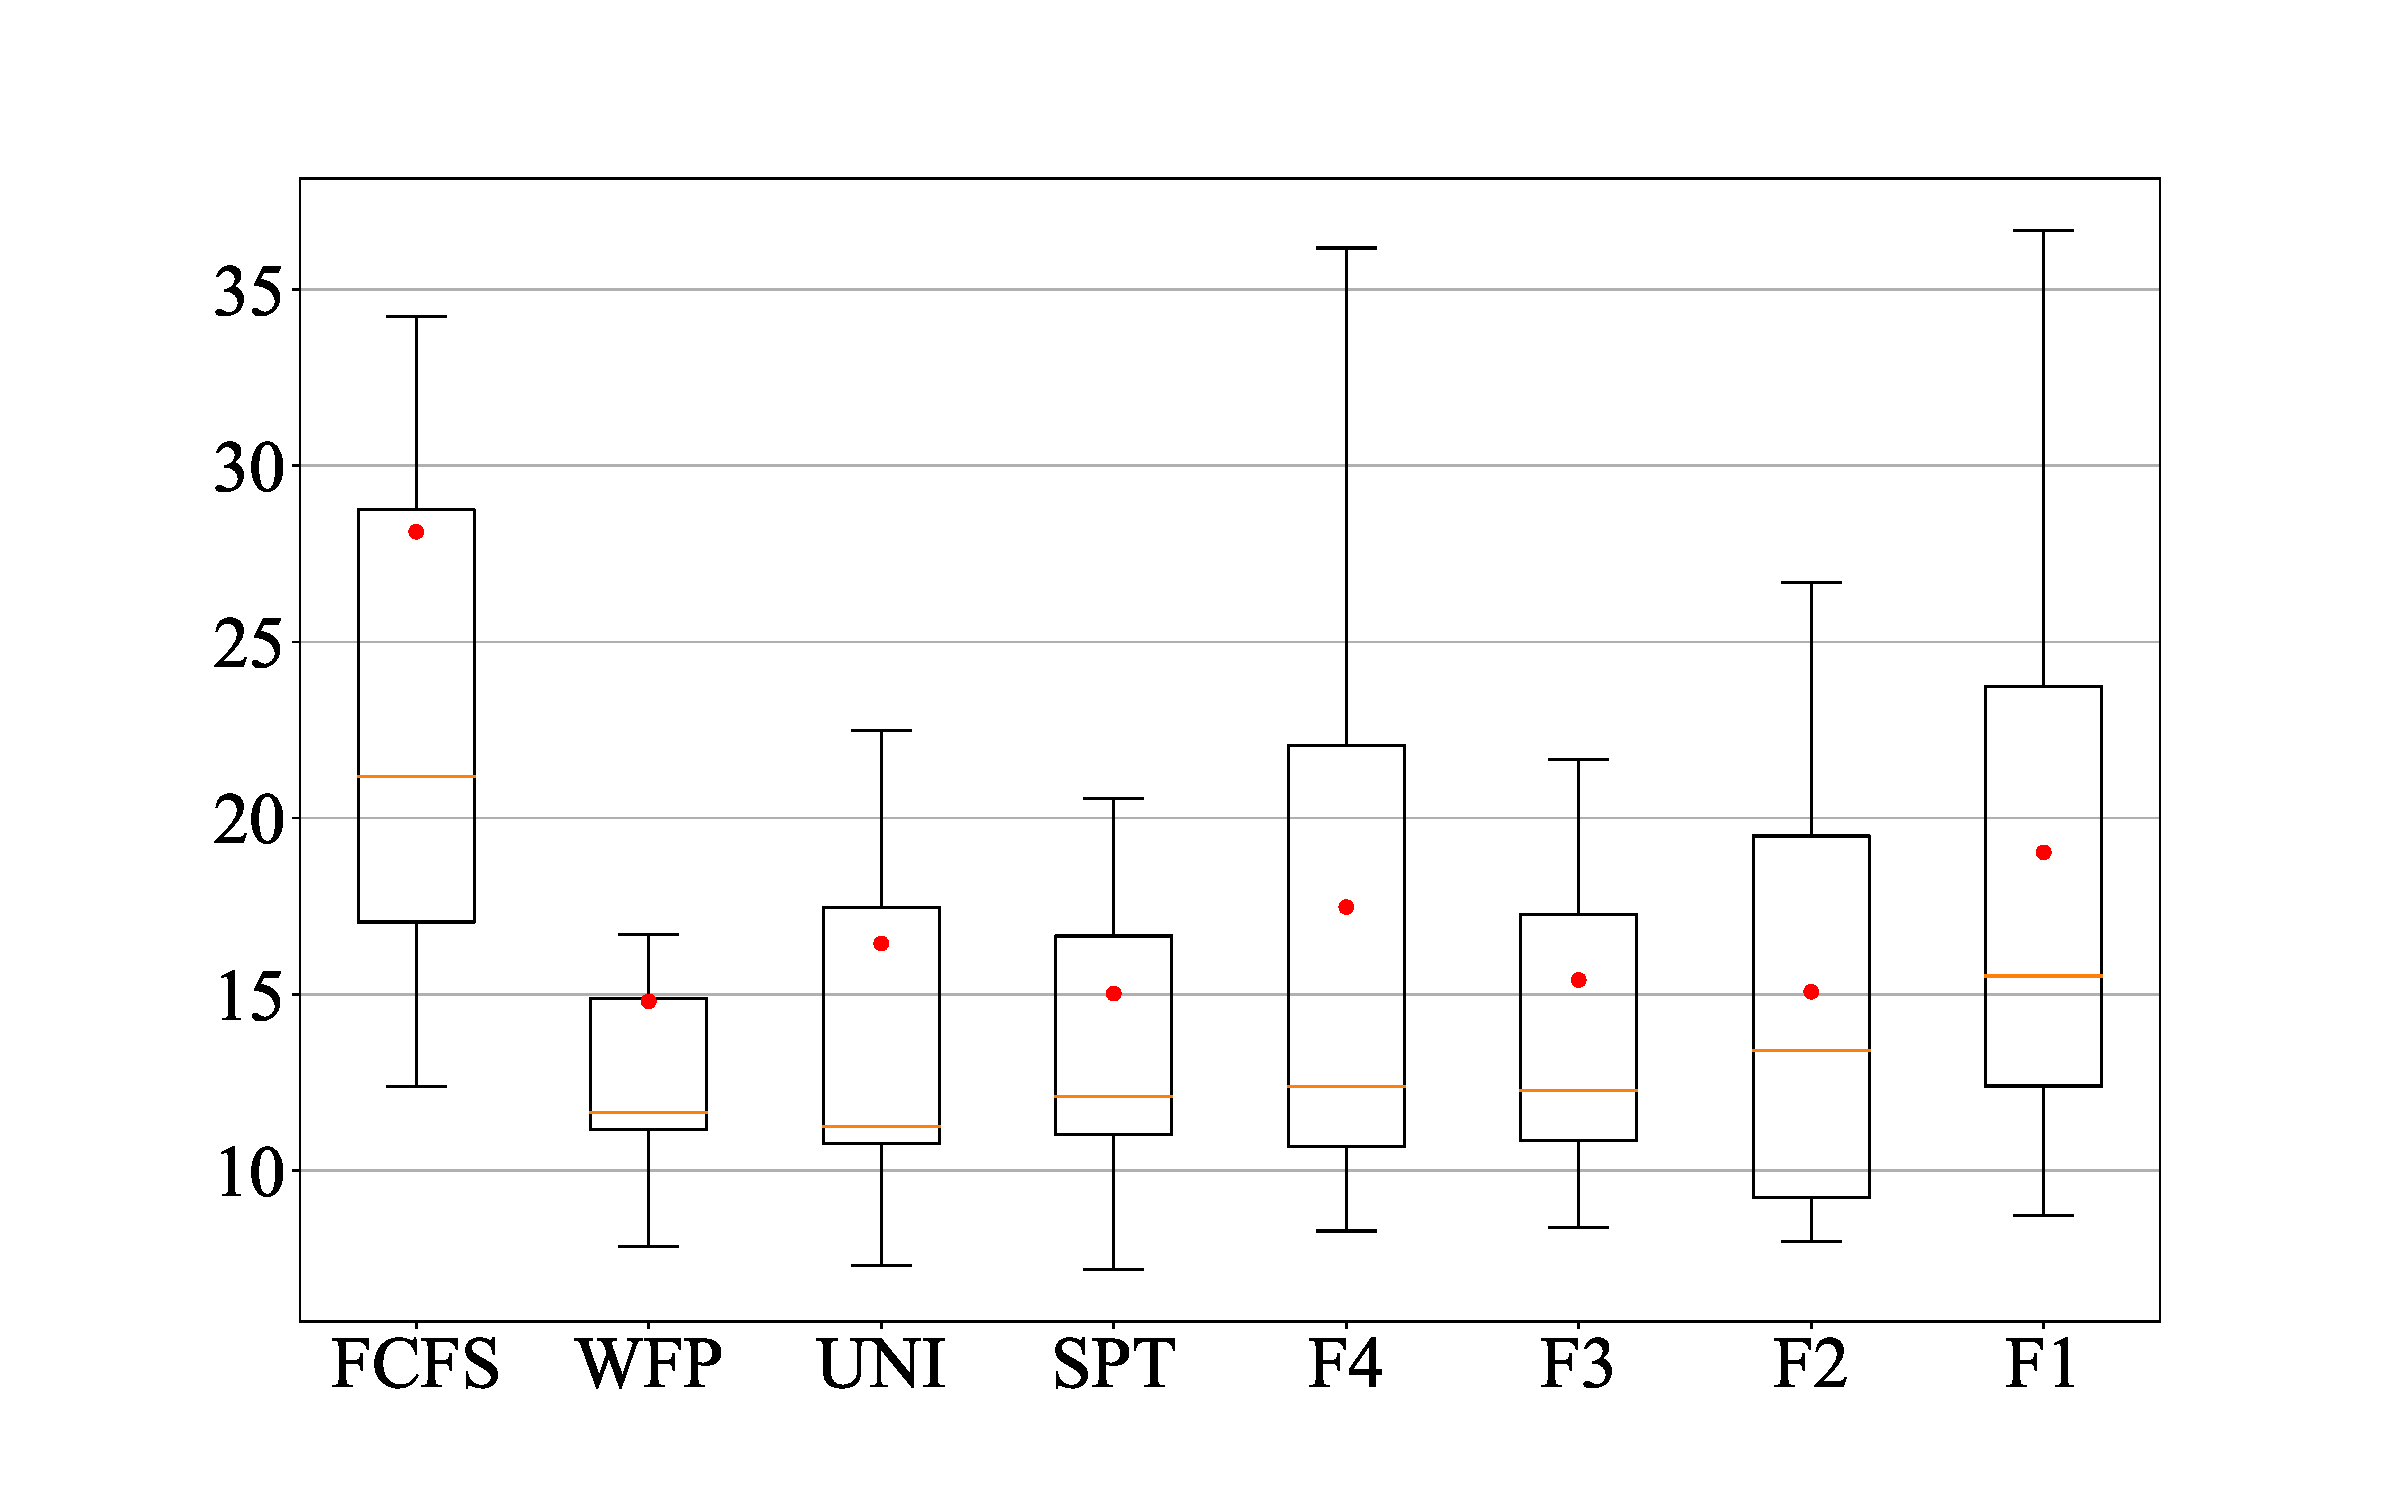
\includegraphics[scale=.20]{figs/Fig10a.pdf}
			%\caption{fig1}
		\end{minipage}%
	}%
	\subfigure[$A\!V\!Gblsd$ with predicted time]{
		\begin{minipage}[t]{0.44\linewidth}
			\centering
			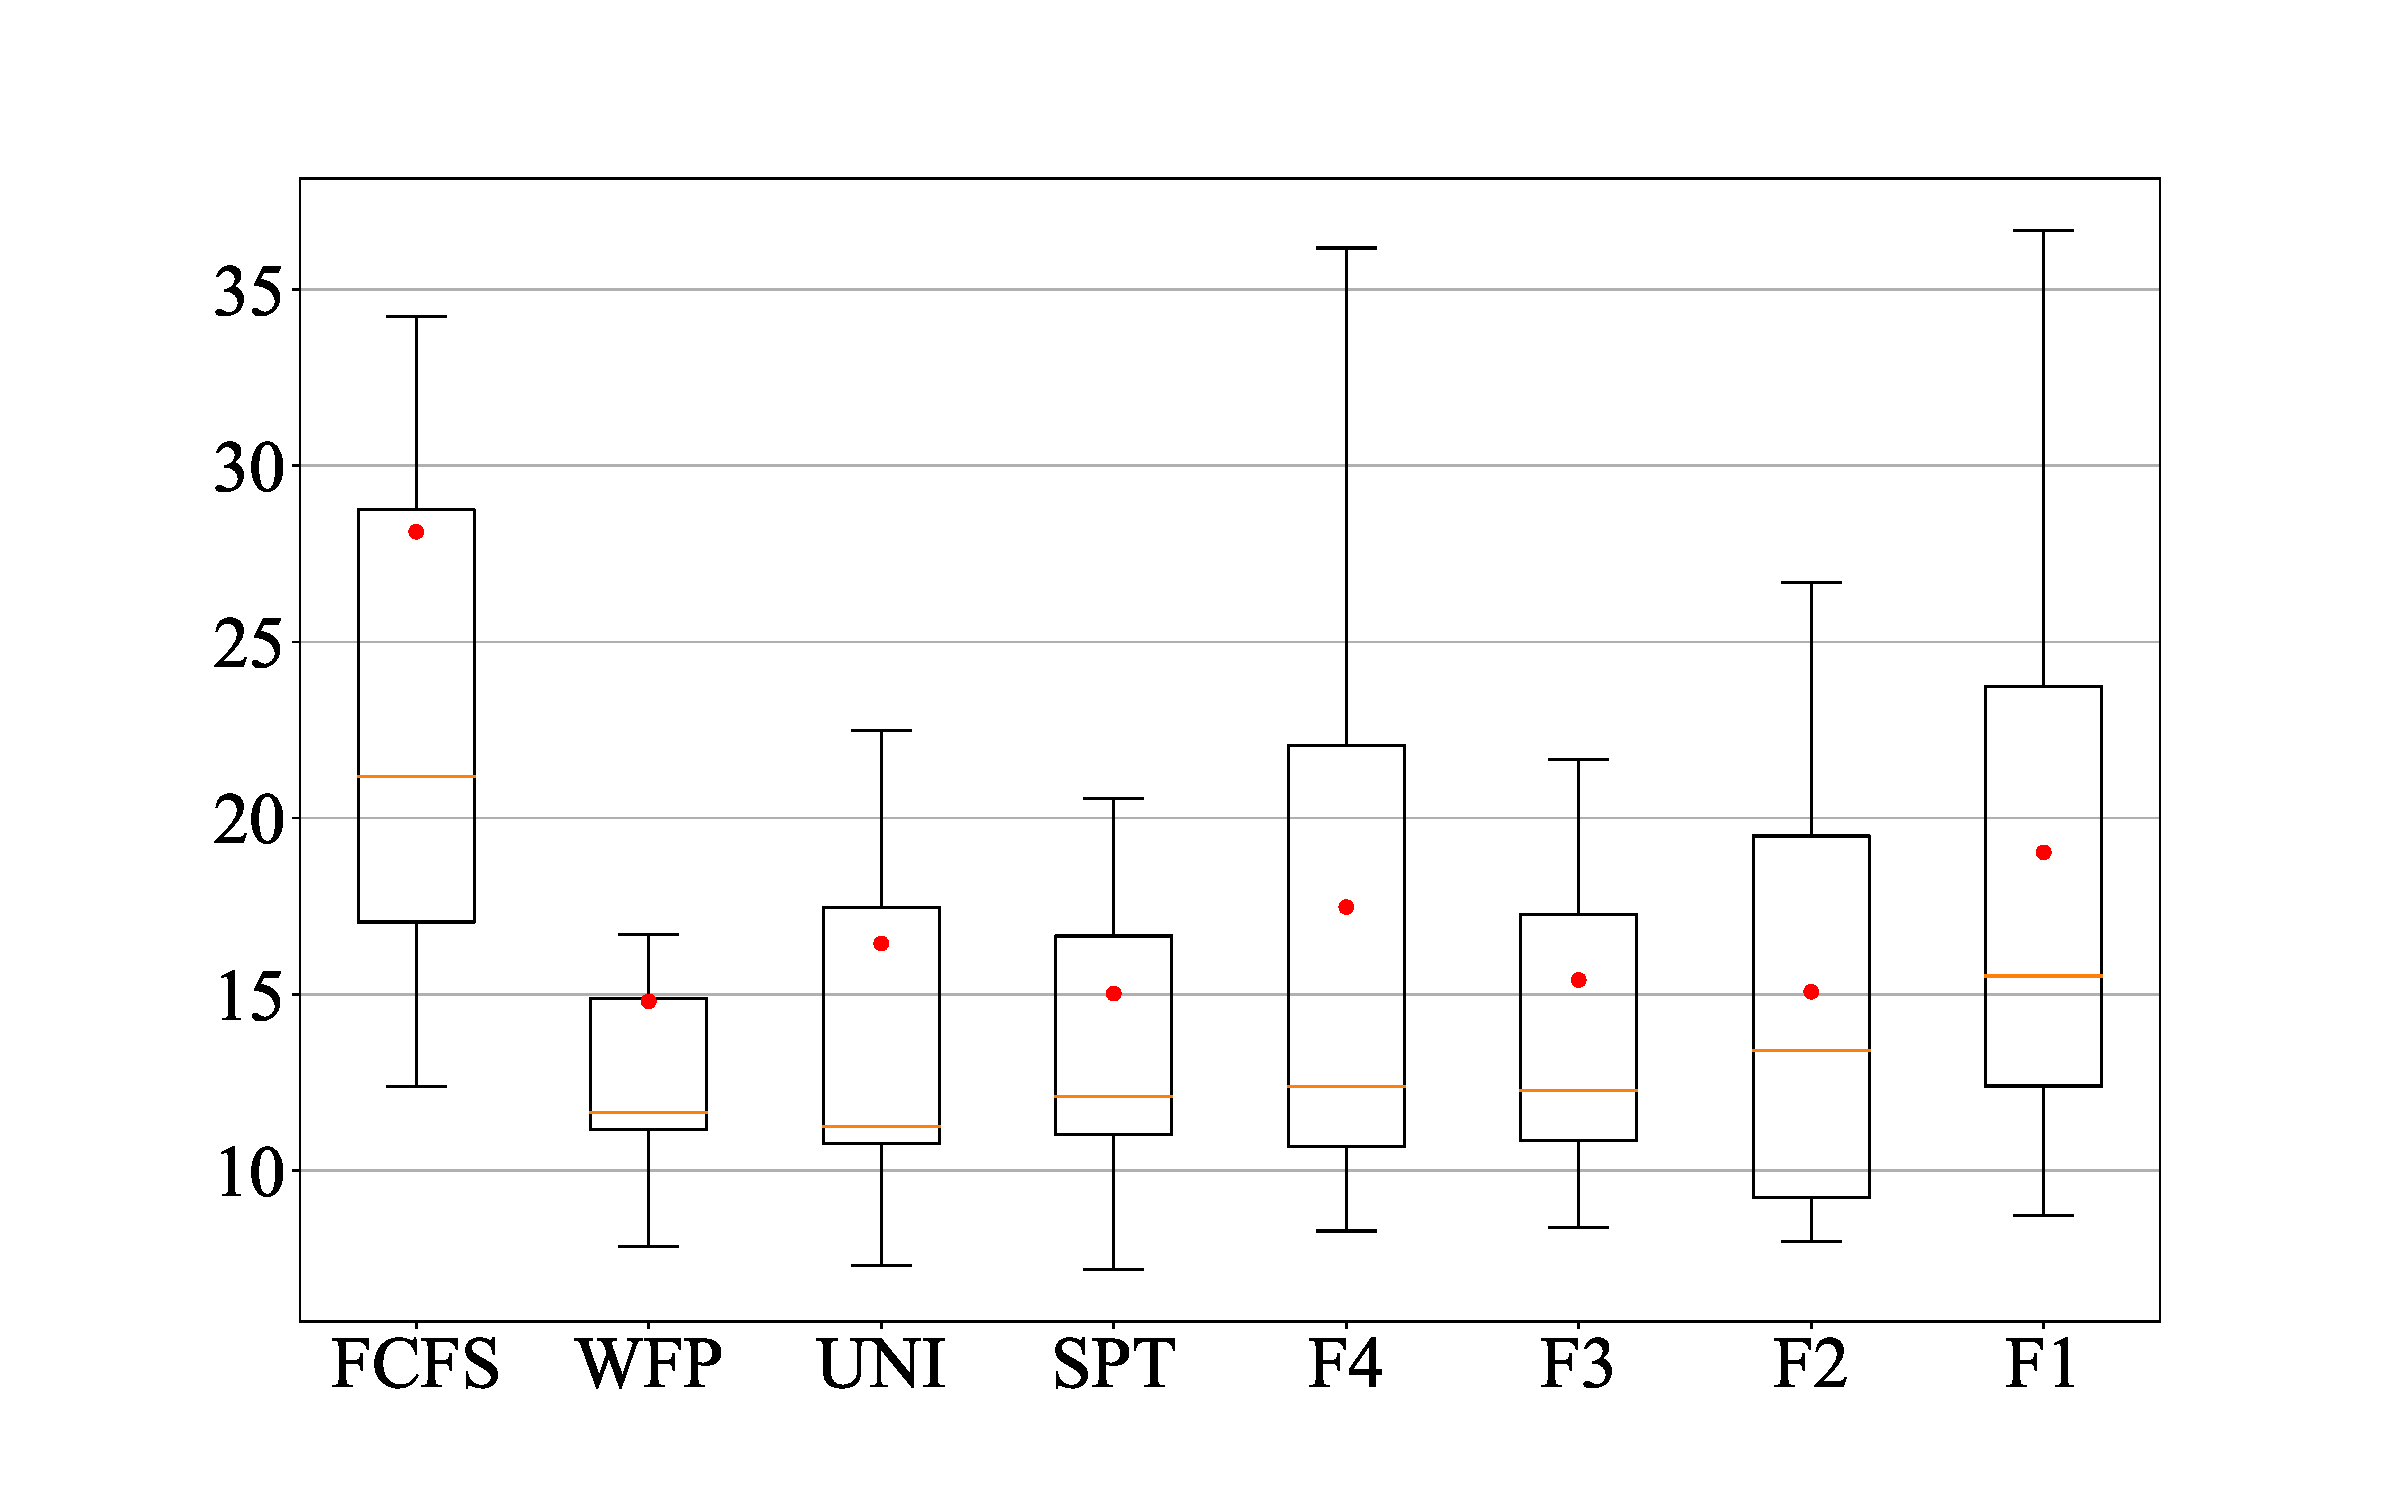
\includegraphics[scale=.20]{figs/Fig10b.pdf}
			%\caption{fig2}
		\end{minipage}%
	}%
	\, %这个回车键很重要 \quad也可以
	\subfigure[$A\!V\!Gwt$ with user-requested time]{
		\begin{minipage}[t]{0.44\linewidth}
			\centering
			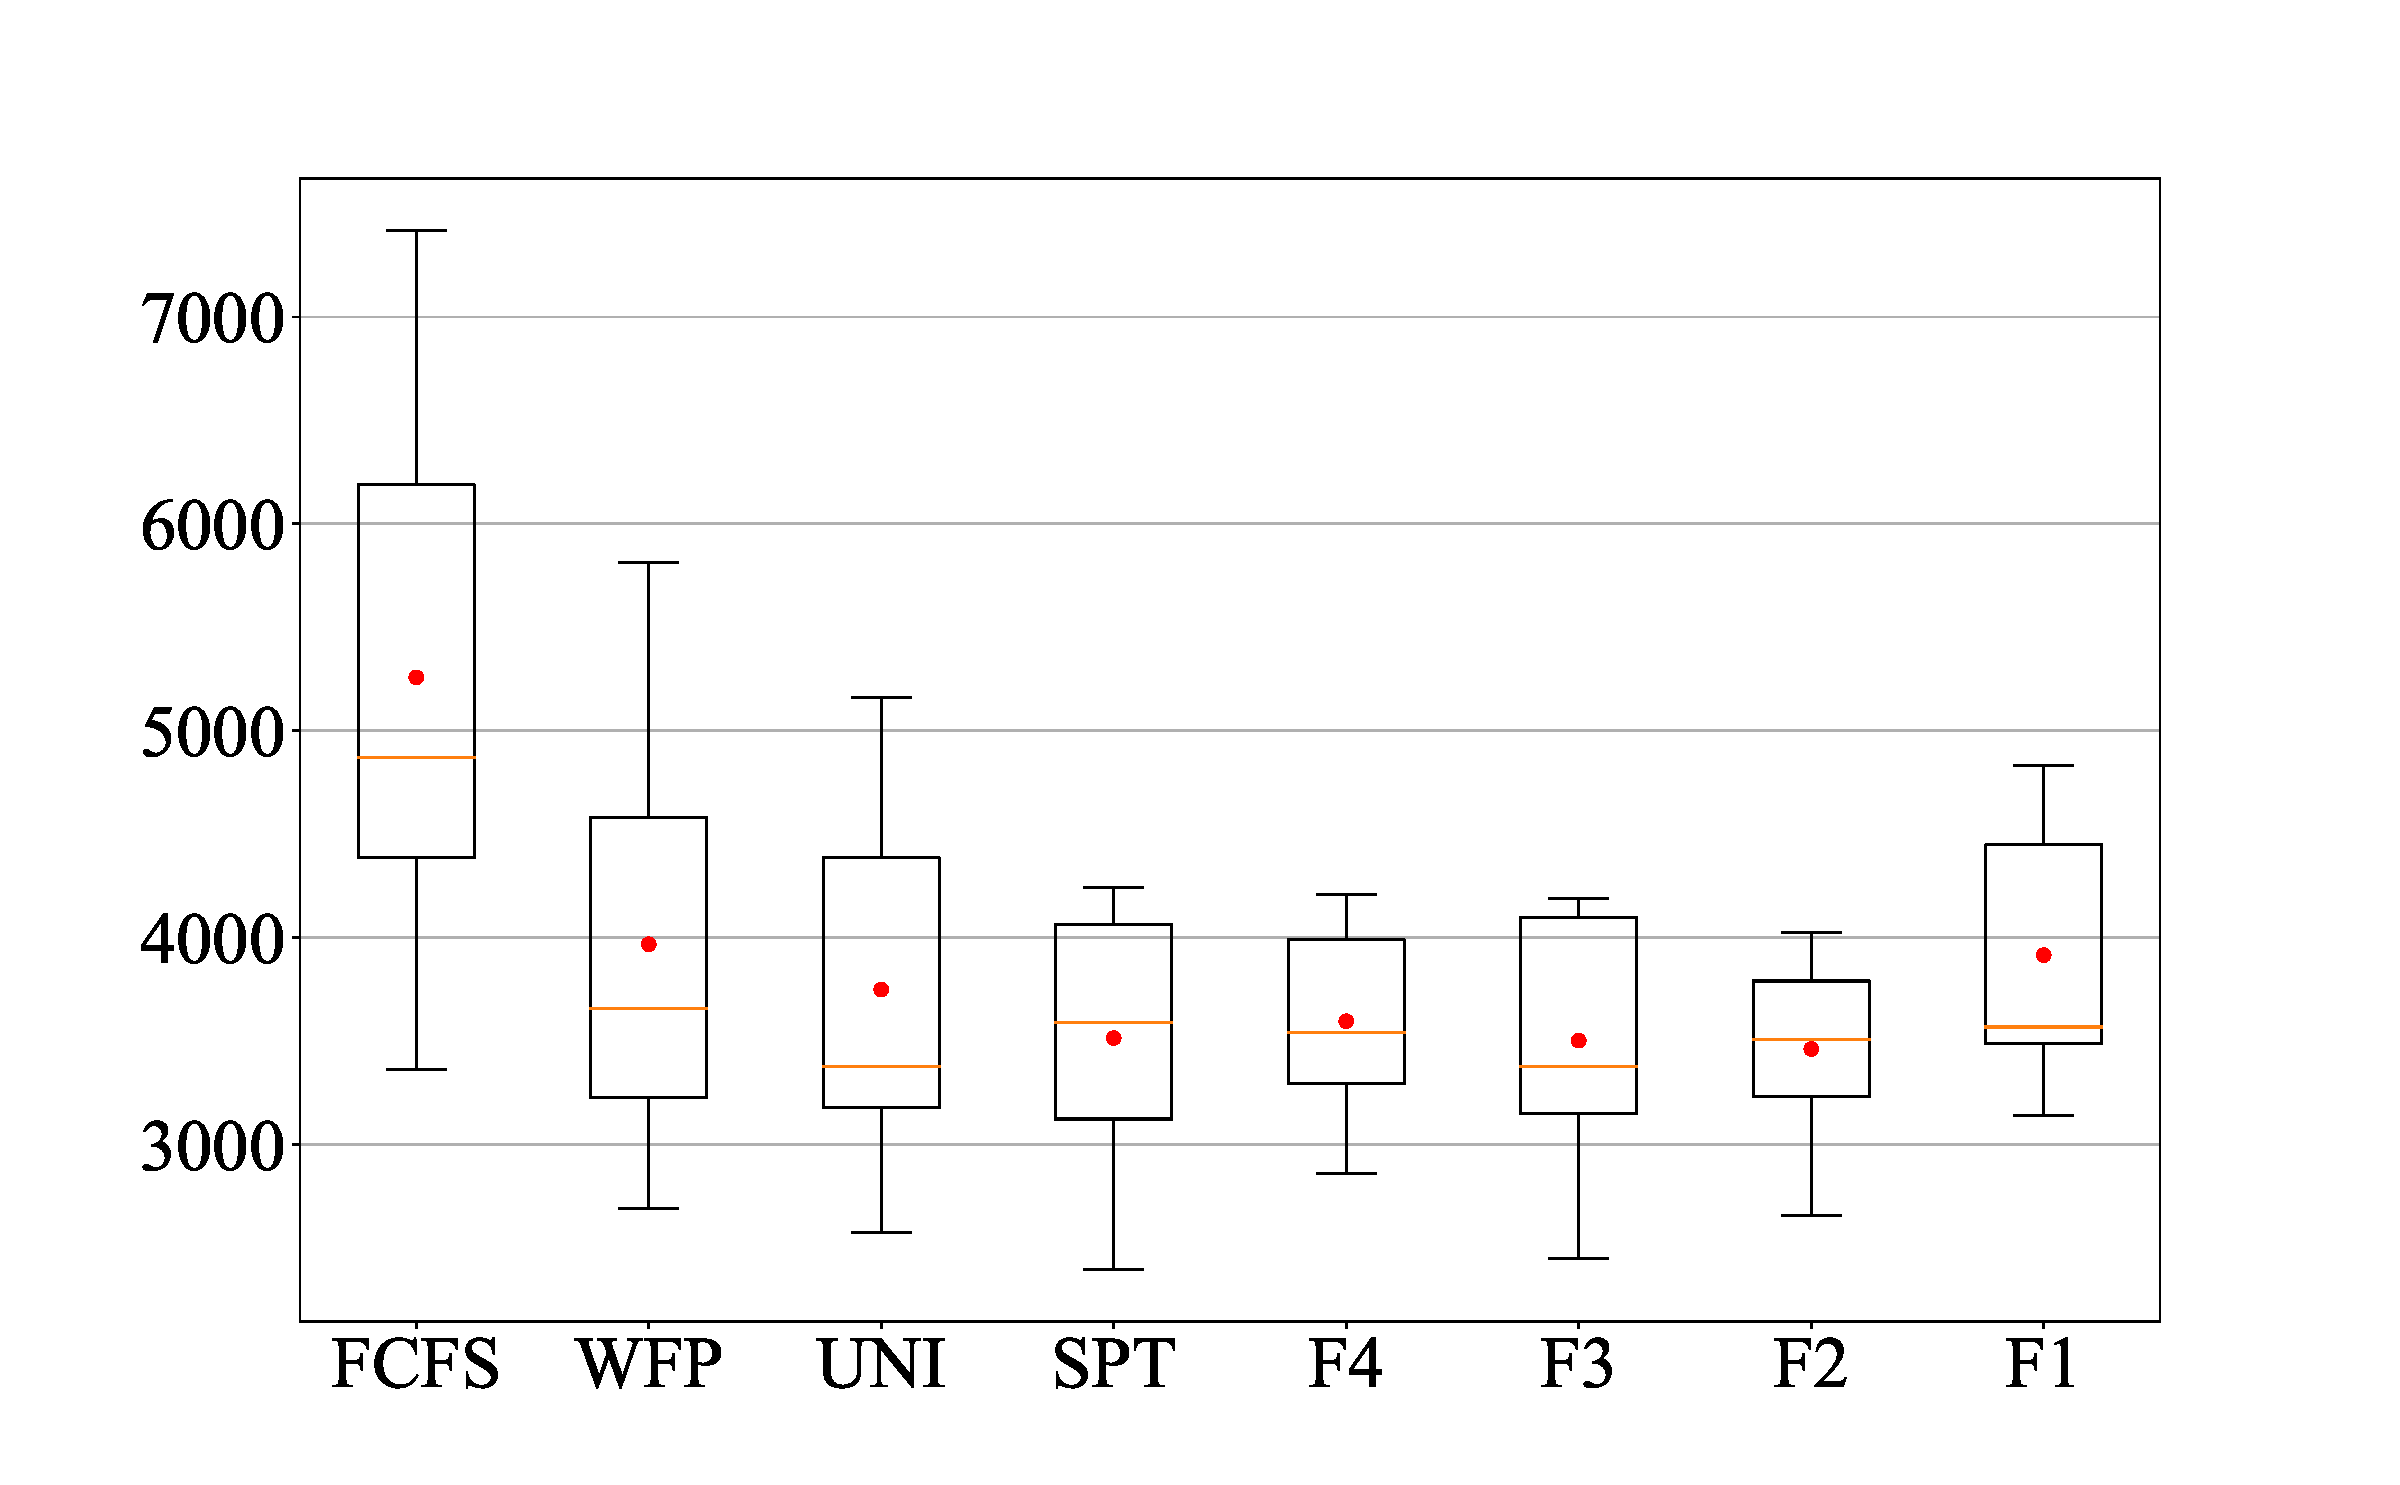
\includegraphics[scale=.20]{figs/Fig10c.pdf}
			%\caption{fig2}
		\end{minipage}
	}%
	\subfigure[$A\!V\!Gwt$ with predicted time]{
		\begin{minipage}[t]{0.44\linewidth}
			\centering
			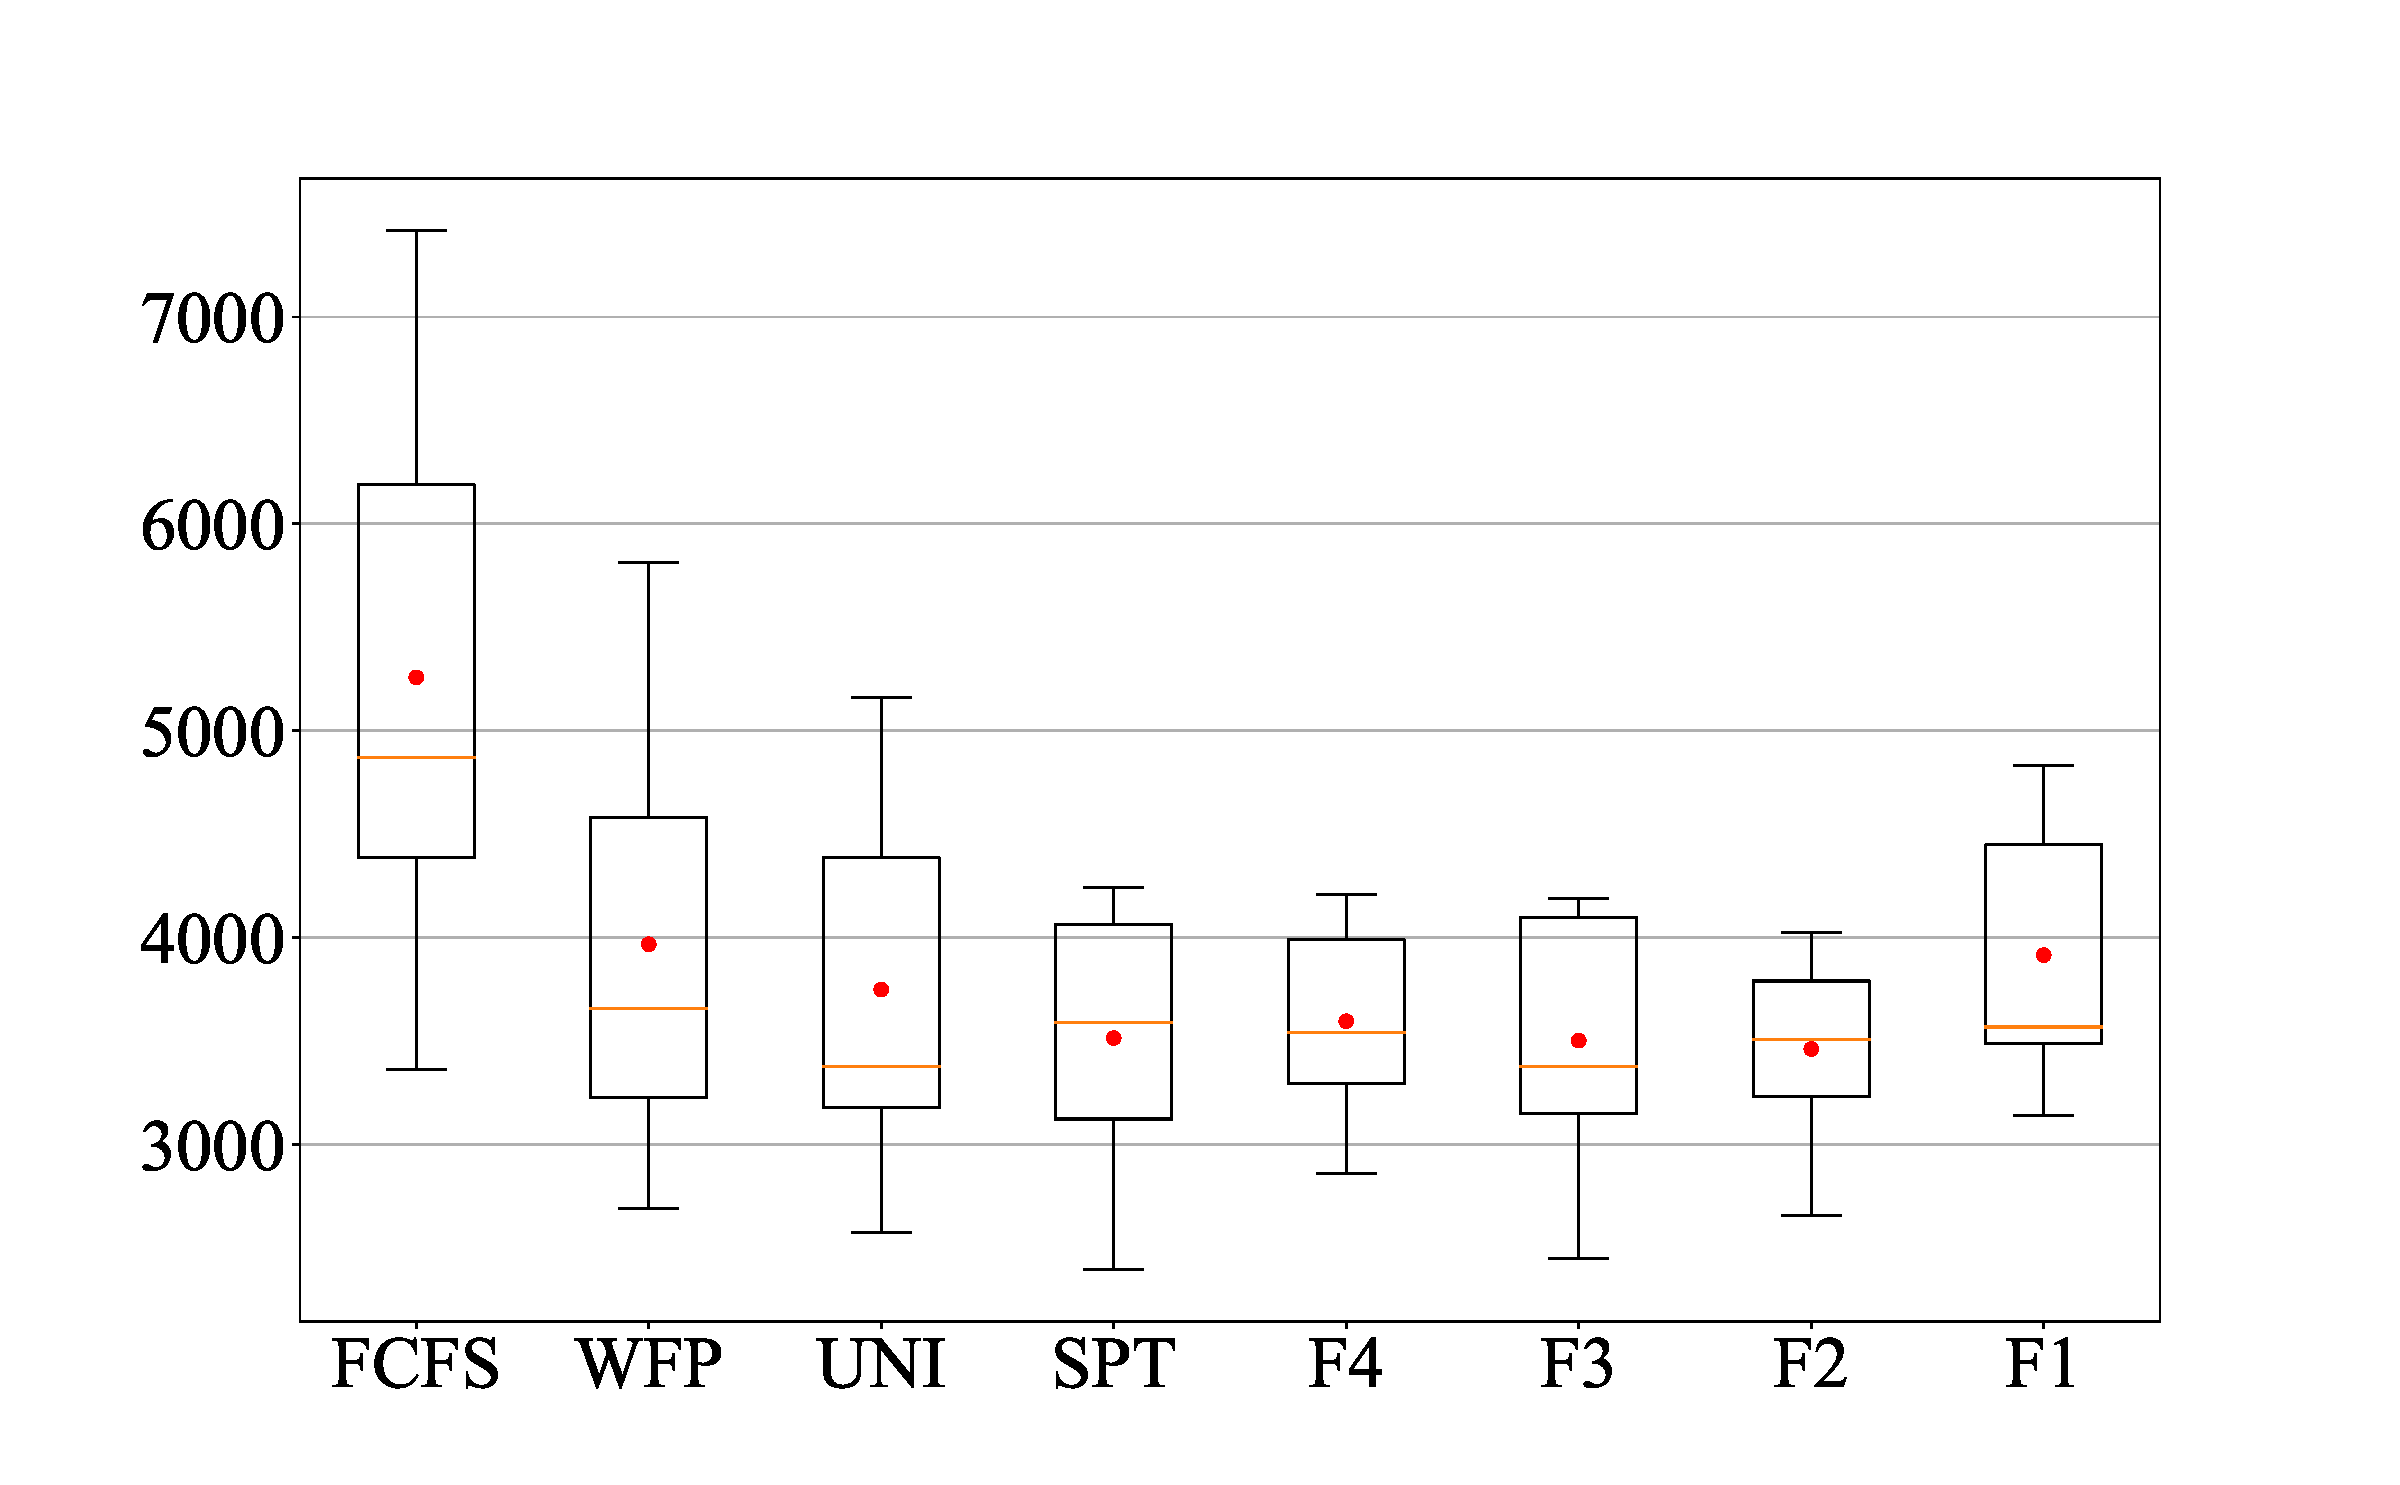
\includegraphics[scale=.20]{figs/Fig10d.pdf}
			%\caption{fig2}
		\end{minipage}
	}%	
	\centering
	\caption{SDSC-SP2 workload scheduling performance.} \label{Fig:10}
\end{figure}
Figure \ref{Fig:10} shows the scheduling result of the SDSC-SP2-1998-4.2-cln workload, and Tables \ref{tbl15}-\ref{tbl18} are the corresponding median and mean values of $A\!V\!Gblsd$ and $A\!V\!Gwt$ with user-requested time and predicted time, respectively.
\begin{table}[width=.62\linewidth,cols=9,pos=h]
	\caption{Median and mean $A\!V\!Gblsd$ scheduling performance with $t_{req}$ of SDSC-SP2 workload.}\label{tbl15}
	\begin{tabular*}{\tblwidth}{@{} LLLLLLLLL@{} }
		\toprule
		Indicator & FCFS & WFP & UNI & SPT & F4 & F3 & F2 & F1\\
		\midrule
		Median & 21.5 & 16.5 & 14.1 & 17.7 & 13.1 & 12.5 & 15.8 & 17.9 \\
		Mean & 29.9 & 20.7 & 18.9 & 18.4 & 16.7 & 16.5 & 16.3 & 	18.8 \\
		\bottomrule
	\end{tabular*}
\end{table}
\begin{table}[width=.62\linewidth,cols=9,pos=h]
	\caption{Median and mean $A\!V\!Gblsd$ scheduling performance with $t_{pred}$ of SDSC-SP2 workload.}\label{tbl16}
	\begin{tabular*}{\tblwidth}{@{} LLLLLLLLL@{} }
		\toprule
		Indicator & FCFS & WFP & UNI & SPT & F4 & F3 & F2 & F1\\
		\midrule
		Median & 21.1 & 11.6 & \textbf{11.2} & 12.1 & 12.4 & 12.26 & 13.4 & 15.5 \\
		Mean & 28.1 & \textbf{14.8} & 16.4 & 15.0 & 17.5 & 15.4 &  15.1 & 19.0 \\
		\bottomrule
	\end{tabular*}
\end{table}

For the $A\!V\!Gblsd$ of SDSC-SP2-1998-4.2-cln, shown as Table \ref{tbl15} and \ref{tbl16}, except for the mean performance of F4 (decreased by 4.7\%), all scheduling performance parameters are improved by OKCM according to both indicators. For the median value, UNI scheduling obtains the optimal performance, and SPT achieves up to 1.46 times improvement. In terms of mean, WFP has the highest performance, and also achieves a maximum 1.40 times improvement.
\begin{table}[width=.62\linewidth,cols=9,pos=h]
	\caption{Median and mean $A\!V\!Gwt$ scheduling performance with $t_{req}$ of SDSC-SP2 workload.}\label{tbl17}
	\begin{tabular*}{\tblwidth}{@{} LLLLLLLLL@{} }
		\toprule
		Indicator & FCFS & WFP & UNI & SPT & F4 & F3 & F2 & F1\\
		\midrule
		Median & 5168.4 & 4135.5 & 3845.4 & 3406.9 & 3277.5 & 3391.3 & 3685.4 & 4415.9 \\
		Mean & 6009.8 & 4853.5 & 4096.7 & 3622.7 & 3497.0 & 3472.7 & 3649.9 & 4246.3 \\
		\bottomrule
	\end{tabular*}
\end{table}
\begin{table}[width=.62\linewidth,cols=9,pos=h]
	\caption{Median and mean $A\!V\!Gwt$ scheduling performance with $t_{pred}$ of SDSC-SP2 workload.}\label{tbl18}
	\begin{tabular*}{\tblwidth}{@{} LLLLLLLLL@{} }
		\toprule
		Indicator & FCFS & WFP & UNI & SPT & F4 & F3 & F2 & F1\\
		\midrule
		Median & 4868.3 & 3655.3 & \textbf{3373.9} & 3587.5 & 3540.8 & 3376.6 & 3504.9 & 3566.6 \\
		Mean & 5257.4 & 3966.8 & 3747.7 & 3513.0 & 3594.7 & 3500.6 & \textbf{3460.3} & 3914.2 \\
		\bottomrule
	\end{tabular*}
\end{table}

For the $A\!V\!Gwt$ of SDSC-SP2-1998-4.2-cln, shown as Table \ref{tbl17} and \ref{tbl18}, except for the mean performance of SPT (decreased by 5.3\%), the mean of F4 (decreased by 2.8\%), and the mean of F3 (decreased by 0.8\%), all other scheduling performance is improved by OKCM according to both indicators. For the median value, UNI scheduling obtains the optimal performance, and F1 achieves up to 1.24 times improvement. In terms of mean, F2 has the highest performance, and WFP achieves a maximum 1.22 times improvement. 

Scheduling with our prediction runtime resulted in reduced differences between the 25\% and 75\% quartiles in both $A\!V\!Gblsd$ and $A\!V\!Gwt$ for the SDSC-SP2-1998-4.2-cln workload.

\subsubsection{Overview of scheduling performance}
Although the scheduling performance varied depending on the character of the jobs and the platform, the result was usually a significant improvement in performance.
 
Moreover, scheduling with required time produced either a large range of $25^{th}-75^{th}$ percentile box, or outlier points with average slowdowns significantly higher than the median and mean, which damage the quality of service of the HPC system seriously. For all scheduling policy, scheduling with our prediction runtime resulted in reduced differences between the 25\% and 75\% quartiles in both $A\!V\!Gblsd$ and $A\!V\!Gwt$. OKCM can be used to enhance the main prioritizing and backfilling methods and is not limited to a specific type of scheduling.

\section{Conclusion} \label{sect5}
In this study, the OKCM model is proposed to improve the job runtime prediction for the HPC scheduling system. Previous studies and models focus only on improving accuracy, resulting in higher computational complexity, time overhead, and difficult deployment in real-time scheduling systems. Our design updates the model in real time through online learning and is friendly to new users or users with a small amount of data through the KNN-based predictor, which is an important feature for a real system. The correction mechanism is designed to guarantee the safe running of high-priority and subsequent jobs. The trace-driven simulator HPCsim was designed implemented based on real job workloads to evaluate the model. The results demonstrated that OKCM led to important scheduling performance improvements and enhanced primary prioritizing and backfilling methods without scheduling limitations.

In future research, we would improve in two directions. First, we would deploy the model using real HPC platforms and assess performance with real jobs and users. We used a realistic simulation to evaluate the prediction model and its scheduling performance using real traces. However, the traces ignored some important factors, such as memory bottlenecks that could affect job execution. Nevertheless, the simulations are a good approximation of these HPC platforms.

The second direction would be research in a wider range of HPC platforms, containing computing units with distinct architectures such as GPUs \cite{22GPU} and the Sunway TaihuLight-like supercomputer \cite{23Lijingbo}. We plan to continue optimizing the OKCM model to improve scheduling performance of heterogeneous HPC platforms. 

We recommend that when a job is completed, the system pushes the real runtime of the job to the user, so the user can compare the time and provide a more accurate requested time when submitting the next job. This feature has been implemented in our simulator and is found to yield a significantly improved accuracy for user-supplied time.

\section{Declaration of competing interest}
The authors declare that they have no known competing financial interests or personal relationships that could have appeared to influence the work reported in this paper.

\section{Acknowledgments}
This research was funded by the National Key Research and Development Program of China, grant number: 2016YFB0200902.

%\section{References}

%% Loading bibliography style file
%\bibliographystyle{model1-num-names}
%\bibliographystyle{cas-model2-names}
%\bibliographystyle{plain}
\bibliographystyle{unsrt}
% Loading bibliography database
\bibliography{OKCM-refs}


%\appendix
%\section{Appendix}


\printcredits


%\vskip3pt

\bio{figs/li.jpg}
\textbf{Jingbo Li} is currently a Ph.D. candidate in School of Computer Science and Technology at Xi'an Jiaotong University. He is a student member of CCF. His main research interests include computer architecture, high performance computing, parallel scheduling and machine learning.
\\
\\
\\
\\
\\
\\
\endbio


\bio{figs/zhang.jpg}
\textbf{Xingjun zhang} is currently a Professor in School of Computer Science and Technology at Xi'an Jiaotong University. He is a member of CCF. His research interests mainly include computer architecture, high performance computing, big data storage system and computer networks.
\endbio


\end{document}

